\documentclass[twoside]{book}

% Packages required by doxygen
\usepackage{calc}
\usepackage{doxygen}
\usepackage{graphicx}
\usepackage[utf8]{inputenc}
\usepackage{makeidx}
\usepackage{multicol}
\usepackage{multirow}
\usepackage{textcomp}
\usepackage[table]{xcolor}

% Font selection
\usepackage[T1]{fontenc}
\usepackage{mathptmx}
\usepackage[scaled=.90]{helvet}
\usepackage{courier}
\usepackage{amssymb}
\usepackage{sectsty}
\renewcommand{\familydefault}{\sfdefault}
\allsectionsfont{%
  \fontseries{bc}\selectfont%
  \color{darkgray}%
}
\renewcommand{\DoxyLabelFont}{%
  \fontseries{bc}\selectfont%
  \color{darkgray}%
}

% Page & text layout
\usepackage{geometry}
\geometry{%
  a4paper,%
  top=2.5cm,%
  bottom=2.5cm,%
  left=2.5cm,%
  right=2.5cm%
}
\tolerance=750
\hfuzz=15pt
\hbadness=750
\setlength{\emergencystretch}{15pt}
\setlength{\parindent}{0cm}
\setlength{\parskip}{0.2cm}
\makeatletter
\renewcommand{\paragraph}{%
  \@startsection{paragraph}{4}{0ex}{-1.0ex}{1.0ex}{%
    \normalfont\normalsize\bfseries\SS@parafont%
  }%
}
\renewcommand{\subparagraph}{%
  \@startsection{subparagraph}{5}{0ex}{-1.0ex}{1.0ex}{%
    \normalfont\normalsize\bfseries\SS@subparafont%
  }%
}
\makeatother

% Headers & footers
\usepackage{fancyhdr}
\pagestyle{fancyplain}
\fancyhead[LE]{\fancyplain{}{\bfseries\thepage}}
\fancyhead[CE]{\fancyplain{}{}}
\fancyhead[RE]{\fancyplain{}{\bfseries\leftmark}}
\fancyhead[LO]{\fancyplain{}{\bfseries\rightmark}}
\fancyhead[CO]{\fancyplain{}{}}
\fancyhead[RO]{\fancyplain{}{\bfseries\thepage}}
\fancyfoot[LE]{\fancyplain{}{}}
\fancyfoot[CE]{\fancyplain{}{}}
\fancyfoot[RE]{\fancyplain{}{\bfseries\scriptsize Generated on Fri Jul 17 2015 19\-:06\-:06 for My Project by Doxygen }}
\fancyfoot[LO]{\fancyplain{}{\bfseries\scriptsize Generated on Fri Jul 17 2015 19\-:06\-:06 for My Project by Doxygen }}
\fancyfoot[CO]{\fancyplain{}{}}
\fancyfoot[RO]{\fancyplain{}{}}
\renewcommand{\footrulewidth}{0.4pt}
\renewcommand{\chaptermark}[1]{%
  \markboth{#1}{}%
}
\renewcommand{\sectionmark}[1]{%
  \markright{\thesection\ #1}%
}

% Indices & bibliography
\usepackage{natbib}
\usepackage[titles]{tocloft}
\setcounter{tocdepth}{3}
\setcounter{secnumdepth}{5}
\makeindex

% Hyperlinks (required, but should be loaded last)
\usepackage{ifpdf}
\ifpdf
  \usepackage[pdftex,pagebackref=true]{hyperref}
\else
  \usepackage[ps2pdf,pagebackref=true]{hyperref}
\fi
\hypersetup{%
  colorlinks=true,%
  linkcolor=blue,%
  citecolor=blue,%
  unicode%
}

% Custom commands
\newcommand{\clearemptydoublepage}{%
  \newpage{\pagestyle{empty}\cleardoublepage}%
}


%===== C O N T E N T S =====

\begin{document}

% Titlepage & ToC
\hypersetup{pageanchor=false}
\pagenumbering{roman}
\begin{titlepage}
\vspace*{7cm}
\begin{center}%
{\Large My Project }\\
\vspace*{1cm}
{\large Generated by Doxygen 1.8.6}\\
\vspace*{0.5cm}
{\small Fri Jul 17 2015 19:06:06}\\
\end{center}
\end{titlepage}
\clearemptydoublepage
\tableofcontents
\clearemptydoublepage
\pagenumbering{arabic}
\hypersetup{pageanchor=true}

%--- Begin generated contents ---
\chapter{R\-E\-A\-D\-M\-E}
\label{md_README}
\hypertarget{md_README}{}
Estimate time to completion\-: 25 hours

7-\/11-\/15 5\-:30 -\/ 7\-:00 7-\/12-\/15 3\-:00 -\/ 6\-:00 7-\/12-\/15 9\-:00 -\/ 10\-:30 7-\/13-\/15 7\-:00 -\/ 11\-:00 7-\/14-\/15 3\-:00 -\/ 9\-:00 7-\/14-\/15 4\-:30 -\/ 9\-:30 7-\/15-\/15 4\-:00 -\/ 10\-:00 7-\/16-\/15 5\-:00 -\/ 10\-:00

T\-O\-T\-A\-L\-: 32 
\chapter{Hierarchical Index}
\section{Class Hierarchy}
This inheritance list is sorted roughly, but not completely, alphabetically\-:\begin{DoxyCompactList}
\item \contentsline{section}{my\-\_\-deque$<$ T, A $>$\-:\-:const\-\_\-iterator}{\pageref{classmy__deque_1_1const__iterator}}{}
\item \contentsline{section}{my\-\_\-deque$<$ T, A $>$\-:\-:iterator}{\pageref{classmy__deque_1_1iterator}}{}
\item \contentsline{section}{my\-\_\-deque$<$ T, A $>$}{\pageref{classmy__deque}}{}
\item Test\begin{DoxyCompactList}
\item \contentsline{section}{Deque\-\_\-\-Fixture$<$ T $>$}{\pageref{structDeque__Fixture}}{}
\end{DoxyCompactList}
\end{DoxyCompactList}

\chapter{Class Index}
\section{Class List}
Here are the classes, structs, unions and interfaces with brief descriptions\-:\begin{DoxyCompactList}
\item\contentsline{section}{\hyperlink{classmy__deque_1_1const__iterator}{my\-\_\-deque$<$ T, A $>$\-::const\-\_\-iterator} }{\pageref{classmy__deque_1_1const__iterator}}{}
\item\contentsline{section}{\hyperlink{structDeque__Fixture}{Deque\-\_\-\-Fixture$<$ T $>$} }{\pageref{structDeque__Fixture}}{}
\item\contentsline{section}{\hyperlink{classmy__deque_1_1iterator}{my\-\_\-deque$<$ T, A $>$\-::iterator} }{\pageref{classmy__deque_1_1iterator}}{}
\item\contentsline{section}{\hyperlink{classmy__deque}{my\-\_\-deque$<$ T, A $>$} }{\pageref{classmy__deque}}{}
\end{DoxyCompactList}

\chapter{File Index}
\section{File List}
Here is a list of all files with brief descriptions\-:\begin{DoxyCompactList}
\item\contentsline{section}{\hyperlink{Deque_8h}{Deque.\-h} }{\pageref{Deque_8h}}{}
\item\contentsline{section}{\hyperlink{TestDeque_8c_09_09}{Test\-Deque.\-c++} }{\pageref{TestDeque_8c_09_09}}{}
\end{DoxyCompactList}

\chapter{Class Documentation}
\hypertarget{classmy__deque_1_1const__iterator}{\section{my\-\_\-deque$<$ T, A $>$\-:\-:const\-\_\-iterator Class Reference}
\label{classmy__deque_1_1const__iterator}\index{my\-\_\-deque$<$ T, A $>$\-::const\-\_\-iterator@{my\-\_\-deque$<$ T, A $>$\-::const\-\_\-iterator}}
}


{\ttfamily \#include $<$Deque.\-h$>$}

\subsection*{Public Types}
\begin{DoxyCompactItemize}
\item 
typedef \\*
std\-::bidirectional\-\_\-iterator\-\_\-tag \hyperlink{classmy__deque_1_1const__iterator_a1a84b424e091e49a4af1c13a38621252}{iterator\-\_\-category}
\item 
typedef \hyperlink{classmy__deque_ae9c156c405acc57623a4601ce755596f}{my\-\_\-deque\-::value\-\_\-type} \hyperlink{classmy__deque_1_1const__iterator_adc8d08cb0b0a1dcb50323ba5ab8fdecb}{value\-\_\-type}
\item 
typedef \hyperlink{classmy__deque_ac85676cb2492fbc9bbc6f1a30e9d3c73}{my\-\_\-deque\-::difference\-\_\-type} \hyperlink{classmy__deque_1_1const__iterator_abe3b655aa980c8a12ba486058464c91d}{difference\-\_\-type}
\item 
typedef \hyperlink{classmy__deque_a8fea5edeb2b2cf3dd1246dc3abf9b71b}{my\-\_\-deque\-::const\-\_\-pointer} \hyperlink{classmy__deque_1_1const__iterator_a6a7d42610f3b7e55f38897c151862071}{pointer}
\item 
typedef \hyperlink{classmy__deque_ad50d8b378580088cf77fa43f0640e49c}{my\-\_\-deque\-::const\-\_\-reference} \hyperlink{classmy__deque_1_1const__iterator_a37cd7eef8e73e5a65d7a9d16ba6d3ed2}{reference}
\end{DoxyCompactItemize}
\subsection*{Public Member Functions}
\begin{DoxyCompactItemize}
\item 
\hyperlink{classmy__deque_1_1const__iterator_a0a2f93bb4201408df6cc031a75b01363}{const\-\_\-iterator} (const \hyperlink{classmy__deque}{my\-\_\-deque} $\ast$d, \hyperlink{classmy__deque_a61e5e5317fe72a381ce4d45f09544b02}{size\-\_\-type} s)
\item 
\hyperlink{classmy__deque_1_1const__iterator_a37cd7eef8e73e5a65d7a9d16ba6d3ed2}{reference} \hyperlink{classmy__deque_1_1const__iterator_a14715989004b54dc6a1bcd3d2ac78a20}{operator$\ast$} () const 
\item 
\hyperlink{classmy__deque_1_1const__iterator_a6a7d42610f3b7e55f38897c151862071}{pointer} \hyperlink{classmy__deque_1_1const__iterator_aef7e08cfcebb0c0932422f420645e1ce}{operator-\/$>$} () const 
\item 
\hyperlink{classmy__deque_1_1const__iterator}{const\-\_\-iterator} \& \hyperlink{classmy__deque_1_1const__iterator_a8bc45a394bb73728fca1ebf90755d662}{operator++} ()
\item 
\hyperlink{classmy__deque_1_1const__iterator}{const\-\_\-iterator} \hyperlink{classmy__deque_1_1const__iterator_adf9ea902391ac993088e7c969c64e4de}{operator++} (int)
\item 
\hyperlink{classmy__deque_1_1const__iterator}{const\-\_\-iterator} \& \hyperlink{classmy__deque_1_1const__iterator_ae5dffda4ac0a8ad59a4954dcdeeb5f98}{operator-\/-\/} ()
\item 
\hyperlink{classmy__deque_1_1const__iterator}{const\-\_\-iterator} \hyperlink{classmy__deque_1_1const__iterator_a83c405a1e0b9672c074aaa933a7127df}{operator-\/-\/} (int)
\item 
\hyperlink{classmy__deque_1_1const__iterator}{const\-\_\-iterator} \& \hyperlink{classmy__deque_1_1const__iterator_a2bbc121cc446855edcb9d20451cae024}{operator+=} (\hyperlink{classmy__deque_1_1const__iterator_abe3b655aa980c8a12ba486058464c91d}{difference\-\_\-type} d)
\item 
\hyperlink{classmy__deque_1_1const__iterator}{const\-\_\-iterator} \& \hyperlink{classmy__deque_1_1const__iterator_ab51576a76fd33fd55be87ca4c467dc96}{operator-\/=} (\hyperlink{classmy__deque_1_1const__iterator_abe3b655aa980c8a12ba486058464c91d}{difference\-\_\-type} d)
\end{DoxyCompactItemize}
\subsection*{Private Member Functions}
\begin{DoxyCompactItemize}
\item 
bool \hyperlink{classmy__deque_1_1const__iterator_ab233485f07a0be8dbc1b41987cc1af42}{valid} () const 
\end{DoxyCompactItemize}
\subsection*{Private Attributes}
\begin{DoxyCompactItemize}
\item 
const \hyperlink{classmy__deque}{my\-\_\-deque} $\ast$ \hyperlink{classmy__deque_1_1const__iterator_ac136929fce63d854c0266a1c3b050c7b}{\-\_\-cd}
\item 
\hyperlink{classmy__deque_a61e5e5317fe72a381ce4d45f09544b02}{size\-\_\-type} \hyperlink{classmy__deque_1_1const__iterator_aef40061c16eedaed0e048f50a380b67d}{\-\_\-cindex}
\end{DoxyCompactItemize}
\subsection*{Friends}
\begin{DoxyCompactItemize}
\item 
bool \hyperlink{classmy__deque_1_1const__iterator_a772a728ee48f5cb8904aaae842b0eb82}{operator==} (const \hyperlink{classmy__deque_1_1const__iterator}{const\-\_\-iterator} \&lhs, const \hyperlink{classmy__deque_1_1const__iterator}{const\-\_\-iterator} \&rhs)
\item 
bool \hyperlink{classmy__deque_1_1const__iterator_a12d66edf831aeec4957931d7f7945d90}{operator!=} (const \hyperlink{classmy__deque_1_1const__iterator}{const\-\_\-iterator} \&lhs, const \hyperlink{classmy__deque_1_1const__iterator}{const\-\_\-iterator} \&rhs)
\item 
\hyperlink{classmy__deque_1_1const__iterator}{const\-\_\-iterator} \hyperlink{classmy__deque_1_1const__iterator_ab6ce7b11eff6ef34762c30e4e96a86a0}{operator+} (\hyperlink{classmy__deque_1_1const__iterator}{const\-\_\-iterator} lhs, \hyperlink{classmy__deque_1_1const__iterator_abe3b655aa980c8a12ba486058464c91d}{difference\-\_\-type} rhs)
\item 
\hyperlink{classmy__deque_1_1const__iterator}{const\-\_\-iterator} \hyperlink{classmy__deque_1_1const__iterator_a41934331896eac6321161ff28c21fb29}{operator-\/} (\hyperlink{classmy__deque_1_1const__iterator}{const\-\_\-iterator} lhs, \hyperlink{classmy__deque_1_1const__iterator_abe3b655aa980c8a12ba486058464c91d}{difference\-\_\-type} rhs)
\end{DoxyCompactItemize}


\subsection{Member Typedef Documentation}
\hypertarget{classmy__deque_1_1const__iterator_abe3b655aa980c8a12ba486058464c91d}{\index{my\-\_\-deque\-::const\-\_\-iterator@{my\-\_\-deque\-::const\-\_\-iterator}!difference\-\_\-type@{difference\-\_\-type}}
\index{difference\-\_\-type@{difference\-\_\-type}!my_deque::const_iterator@{my\-\_\-deque\-::const\-\_\-iterator}}
\subsubsection[{difference\-\_\-type}]{\setlength{\rightskip}{0pt plus 5cm}template$<$typename T , typename A  = std\-::allocator$<$\-T$>$$>$ typedef {\bf my\-\_\-deque\-::difference\-\_\-type} {\bf my\-\_\-deque}$<$ T, A $>$\-::{\bf const\-\_\-iterator\-::difference\-\_\-type}}}\label{classmy__deque_1_1const__iterator_abe3b655aa980c8a12ba486058464c91d}
\hypertarget{classmy__deque_1_1const__iterator_a1a84b424e091e49a4af1c13a38621252}{\index{my\-\_\-deque\-::const\-\_\-iterator@{my\-\_\-deque\-::const\-\_\-iterator}!iterator\-\_\-category@{iterator\-\_\-category}}
\index{iterator\-\_\-category@{iterator\-\_\-category}!my_deque::const_iterator@{my\-\_\-deque\-::const\-\_\-iterator}}
\subsubsection[{iterator\-\_\-category}]{\setlength{\rightskip}{0pt plus 5cm}template$<$typename T , typename A  = std\-::allocator$<$\-T$>$$>$ typedef std\-::bidirectional\-\_\-iterator\-\_\-tag {\bf my\-\_\-deque}$<$ T, A $>$\-::{\bf const\-\_\-iterator\-::iterator\-\_\-category}}}\label{classmy__deque_1_1const__iterator_a1a84b424e091e49a4af1c13a38621252}
\hypertarget{classmy__deque_1_1const__iterator_a6a7d42610f3b7e55f38897c151862071}{\index{my\-\_\-deque\-::const\-\_\-iterator@{my\-\_\-deque\-::const\-\_\-iterator}!pointer@{pointer}}
\index{pointer@{pointer}!my_deque::const_iterator@{my\-\_\-deque\-::const\-\_\-iterator}}
\subsubsection[{pointer}]{\setlength{\rightskip}{0pt plus 5cm}template$<$typename T , typename A  = std\-::allocator$<$\-T$>$$>$ typedef {\bf my\-\_\-deque\-::const\-\_\-pointer} {\bf my\-\_\-deque}$<$ T, A $>$\-::{\bf const\-\_\-iterator\-::pointer}}}\label{classmy__deque_1_1const__iterator_a6a7d42610f3b7e55f38897c151862071}
\hypertarget{classmy__deque_1_1const__iterator_a37cd7eef8e73e5a65d7a9d16ba6d3ed2}{\index{my\-\_\-deque\-::const\-\_\-iterator@{my\-\_\-deque\-::const\-\_\-iterator}!reference@{reference}}
\index{reference@{reference}!my_deque::const_iterator@{my\-\_\-deque\-::const\-\_\-iterator}}
\subsubsection[{reference}]{\setlength{\rightskip}{0pt plus 5cm}template$<$typename T , typename A  = std\-::allocator$<$\-T$>$$>$ typedef {\bf my\-\_\-deque\-::const\-\_\-reference} {\bf my\-\_\-deque}$<$ T, A $>$\-::{\bf const\-\_\-iterator\-::reference}}}\label{classmy__deque_1_1const__iterator_a37cd7eef8e73e5a65d7a9d16ba6d3ed2}
\hypertarget{classmy__deque_1_1const__iterator_adc8d08cb0b0a1dcb50323ba5ab8fdecb}{\index{my\-\_\-deque\-::const\-\_\-iterator@{my\-\_\-deque\-::const\-\_\-iterator}!value\-\_\-type@{value\-\_\-type}}
\index{value\-\_\-type@{value\-\_\-type}!my_deque::const_iterator@{my\-\_\-deque\-::const\-\_\-iterator}}
\subsubsection[{value\-\_\-type}]{\setlength{\rightskip}{0pt plus 5cm}template$<$typename T , typename A  = std\-::allocator$<$\-T$>$$>$ typedef {\bf my\-\_\-deque\-::value\-\_\-type} {\bf my\-\_\-deque}$<$ T, A $>$\-::{\bf const\-\_\-iterator\-::value\-\_\-type}}}\label{classmy__deque_1_1const__iterator_adc8d08cb0b0a1dcb50323ba5ab8fdecb}


\subsection{Constructor \& Destructor Documentation}
\hypertarget{classmy__deque_1_1const__iterator_a0a2f93bb4201408df6cc031a75b01363}{\index{my\-\_\-deque\-::const\-\_\-iterator@{my\-\_\-deque\-::const\-\_\-iterator}!const\-\_\-iterator@{const\-\_\-iterator}}
\index{const\-\_\-iterator@{const\-\_\-iterator}!my_deque::const_iterator@{my\-\_\-deque\-::const\-\_\-iterator}}
\subsubsection[{const\-\_\-iterator}]{\setlength{\rightskip}{0pt plus 5cm}template$<$typename T , typename A  = std\-::allocator$<$\-T$>$$>$ {\bf my\-\_\-deque}$<$ T, A $>$\-::const\-\_\-iterator\-::const\-\_\-iterator (
\begin{DoxyParamCaption}
\item[{const {\bf my\-\_\-deque} $\ast$}]{d, }
\item[{{\bf size\-\_\-type}}]{s}
\end{DoxyParamCaption}
)\hspace{0.3cm}{\ttfamily [inline]}}}\label{classmy__deque_1_1const__iterator_a0a2f93bb4201408df6cc031a75b01363}
\hyperlink{classmy__deque_1_1const__iterator}{const\-\_\-iterator} constructor 
\begin{DoxyParams}{Parameters}
{\em const} & \hyperlink{classmy__deque}{my\-\_\-deque} d \\
\hline
{\em size\-\_\-type} & s, index iterator will point to within d \\
\hline
\end{DoxyParams}
\begin{DoxyReturn}{Returns}
\hyperlink{classmy__deque_1_1const__iterator}{const\-\_\-iterator} pointing to const \hyperlink{classmy__deque}{my\-\_\-deque} d at position s 
\end{DoxyReturn}


\subsection{Member Function Documentation}
\hypertarget{classmy__deque_1_1const__iterator_a14715989004b54dc6a1bcd3d2ac78a20}{\index{my\-\_\-deque\-::const\-\_\-iterator@{my\-\_\-deque\-::const\-\_\-iterator}!operator$\ast$@{operator$\ast$}}
\index{operator$\ast$@{operator$\ast$}!my_deque::const_iterator@{my\-\_\-deque\-::const\-\_\-iterator}}
\subsubsection[{operator$\ast$}]{\setlength{\rightskip}{0pt plus 5cm}template$<$typename T , typename A  = std\-::allocator$<$\-T$>$$>$ {\bf reference} {\bf my\-\_\-deque}$<$ T, A $>$\-::const\-\_\-iterator\-::operator$\ast$ (
\begin{DoxyParamCaption}
{}
\end{DoxyParamCaption}
) const\hspace{0.3cm}{\ttfamily [inline]}}}\label{classmy__deque_1_1const__iterator_a14715989004b54dc6a1bcd3d2ac78a20}
\begin{DoxyReturn}{Returns}
reference, element at \-\_\-cindex of \-\_\-cd 
\end{DoxyReturn}
\hypertarget{classmy__deque_1_1const__iterator_a8bc45a394bb73728fca1ebf90755d662}{\index{my\-\_\-deque\-::const\-\_\-iterator@{my\-\_\-deque\-::const\-\_\-iterator}!operator++@{operator++}}
\index{operator++@{operator++}!my_deque::const_iterator@{my\-\_\-deque\-::const\-\_\-iterator}}
\subsubsection[{operator++}]{\setlength{\rightskip}{0pt plus 5cm}template$<$typename T , typename A  = std\-::allocator$<$\-T$>$$>$ {\bf const\-\_\-iterator}\& {\bf my\-\_\-deque}$<$ T, A $>$\-::const\-\_\-iterator\-::operator++ (
\begin{DoxyParamCaption}
{}
\end{DoxyParamCaption}
)\hspace{0.3cm}{\ttfamily [inline]}}}\label{classmy__deque_1_1const__iterator_a8bc45a394bb73728fca1ebf90755d662}
Pre-\/fix ++ \begin{DoxyReturn}{Returns}
\hyperlink{classmy__deque_1_1const__iterator}{const\-\_\-iterator} with updated \-\_\-cindex value 
\end{DoxyReturn}
\hypertarget{classmy__deque_1_1const__iterator_adf9ea902391ac993088e7c969c64e4de}{\index{my\-\_\-deque\-::const\-\_\-iterator@{my\-\_\-deque\-::const\-\_\-iterator}!operator++@{operator++}}
\index{operator++@{operator++}!my_deque::const_iterator@{my\-\_\-deque\-::const\-\_\-iterator}}
\subsubsection[{operator++}]{\setlength{\rightskip}{0pt plus 5cm}template$<$typename T , typename A  = std\-::allocator$<$\-T$>$$>$ {\bf const\-\_\-iterator} {\bf my\-\_\-deque}$<$ T, A $>$\-::const\-\_\-iterator\-::operator++ (
\begin{DoxyParamCaption}
\item[{int}]{}
\end{DoxyParamCaption}
)\hspace{0.3cm}{\ttfamily [inline]}}}\label{classmy__deque_1_1const__iterator_adf9ea902391ac993088e7c969c64e4de}
Post-\/fix ++ 
\begin{DoxyParams}{Parameters}
{\em int} & \\
\hline
\end{DoxyParams}
\begin{DoxyReturn}{Returns}
\hyperlink{classmy__deque_1_1const__iterator}{const\-\_\-iterator} this with previous value, but updates \-\_\-cindex internally 
\end{DoxyReturn}
\hypertarget{classmy__deque_1_1const__iterator_a2bbc121cc446855edcb9d20451cae024}{\index{my\-\_\-deque\-::const\-\_\-iterator@{my\-\_\-deque\-::const\-\_\-iterator}!operator+=@{operator+=}}
\index{operator+=@{operator+=}!my_deque::const_iterator@{my\-\_\-deque\-::const\-\_\-iterator}}
\subsubsection[{operator+=}]{\setlength{\rightskip}{0pt plus 5cm}template$<$typename T , typename A  = std\-::allocator$<$\-T$>$$>$ {\bf const\-\_\-iterator}\& {\bf my\-\_\-deque}$<$ T, A $>$\-::const\-\_\-iterator\-::operator+= (
\begin{DoxyParamCaption}
\item[{{\bf difference\-\_\-type}}]{d}
\end{DoxyParamCaption}
)\hspace{0.3cm}{\ttfamily [inline]}}}\label{classmy__deque_1_1const__iterator_a2bbc121cc446855edcb9d20451cae024}

\begin{DoxyParams}{Parameters}
{\em difference\-\_\-type} & d, the value to be added from \hyperlink{classmy__deque_1_1const__iterator}{const\-\_\-iterator} \\
\hline
\end{DoxyParams}
\begin{DoxyReturn}{Returns}
\hyperlink{classmy__deque_1_1const__iterator}{const\-\_\-iterator} this, with updated \-\_\-cindex value 
\end{DoxyReturn}
\hypertarget{classmy__deque_1_1const__iterator_ae5dffda4ac0a8ad59a4954dcdeeb5f98}{\index{my\-\_\-deque\-::const\-\_\-iterator@{my\-\_\-deque\-::const\-\_\-iterator}!operator-\/-\/@{operator-\/-\/}}
\index{operator-\/-\/@{operator-\/-\/}!my_deque::const_iterator@{my\-\_\-deque\-::const\-\_\-iterator}}
\subsubsection[{operator-\/-\/}]{\setlength{\rightskip}{0pt plus 5cm}template$<$typename T , typename A  = std\-::allocator$<$\-T$>$$>$ {\bf const\-\_\-iterator}\& {\bf my\-\_\-deque}$<$ T, A $>$\-::const\-\_\-iterator\-::operator-\/-\/ (
\begin{DoxyParamCaption}
{}
\end{DoxyParamCaption}
)\hspace{0.3cm}{\ttfamily [inline]}}}\label{classmy__deque_1_1const__iterator_ae5dffda4ac0a8ad59a4954dcdeeb5f98}
Pre-\/fix -- \begin{DoxyReturn}{Returns}
\hyperlink{classmy__deque_1_1const__iterator}{const\-\_\-iterator} this, with updated \-\_\-cindex value 
\end{DoxyReturn}
\hypertarget{classmy__deque_1_1const__iterator_a83c405a1e0b9672c074aaa933a7127df}{\index{my\-\_\-deque\-::const\-\_\-iterator@{my\-\_\-deque\-::const\-\_\-iterator}!operator-\/-\/@{operator-\/-\/}}
\index{operator-\/-\/@{operator-\/-\/}!my_deque::const_iterator@{my\-\_\-deque\-::const\-\_\-iterator}}
\subsubsection[{operator-\/-\/}]{\setlength{\rightskip}{0pt plus 5cm}template$<$typename T , typename A  = std\-::allocator$<$\-T$>$$>$ {\bf const\-\_\-iterator} {\bf my\-\_\-deque}$<$ T, A $>$\-::const\-\_\-iterator\-::operator-\/-\/ (
\begin{DoxyParamCaption}
\item[{int}]{}
\end{DoxyParamCaption}
)\hspace{0.3cm}{\ttfamily [inline]}}}\label{classmy__deque_1_1const__iterator_a83c405a1e0b9672c074aaa933a7127df}
Post-\/fix -- 
\begin{DoxyParams}{Parameters}
{\em int} & \\
\hline
\end{DoxyParams}
\begin{DoxyReturn}{Returns}
\hyperlink{classmy__deque_1_1const__iterator}{const\-\_\-iterator} this with previous value, but updates \-\_\-cindex internally 
\end{DoxyReturn}
\hypertarget{classmy__deque_1_1const__iterator_ab51576a76fd33fd55be87ca4c467dc96}{\index{my\-\_\-deque\-::const\-\_\-iterator@{my\-\_\-deque\-::const\-\_\-iterator}!operator-\/=@{operator-\/=}}
\index{operator-\/=@{operator-\/=}!my_deque::const_iterator@{my\-\_\-deque\-::const\-\_\-iterator}}
\subsubsection[{operator-\/=}]{\setlength{\rightskip}{0pt plus 5cm}template$<$typename T , typename A  = std\-::allocator$<$\-T$>$$>$ {\bf const\-\_\-iterator}\& {\bf my\-\_\-deque}$<$ T, A $>$\-::const\-\_\-iterator\-::operator-\/= (
\begin{DoxyParamCaption}
\item[{{\bf difference\-\_\-type}}]{d}
\end{DoxyParamCaption}
)\hspace{0.3cm}{\ttfamily [inline]}}}\label{classmy__deque_1_1const__iterator_ab51576a76fd33fd55be87ca4c467dc96}

\begin{DoxyParams}{Parameters}
{\em difference\-\_\-type} & d, the value to be subtracted from \hyperlink{classmy__deque_1_1const__iterator}{const\-\_\-iterator} \\
\hline
\end{DoxyParams}
\begin{DoxyReturn}{Returns}
\hyperlink{classmy__deque_1_1const__iterator}{const\-\_\-iterator} this, with updated \-\_\-cindex value 
\end{DoxyReturn}
\hypertarget{classmy__deque_1_1const__iterator_aef7e08cfcebb0c0932422f420645e1ce}{\index{my\-\_\-deque\-::const\-\_\-iterator@{my\-\_\-deque\-::const\-\_\-iterator}!operator-\/$>$@{operator-\/$>$}}
\index{operator-\/$>$@{operator-\/$>$}!my_deque::const_iterator@{my\-\_\-deque\-::const\-\_\-iterator}}
\subsubsection[{operator-\/$>$}]{\setlength{\rightskip}{0pt plus 5cm}template$<$typename T , typename A  = std\-::allocator$<$\-T$>$$>$ {\bf pointer} {\bf my\-\_\-deque}$<$ T, A $>$\-::const\-\_\-iterator\-::operator-\/$>$ (
\begin{DoxyParamCaption}
{}
\end{DoxyParamCaption}
) const\hspace{0.3cm}{\ttfamily [inline]}}}\label{classmy__deque_1_1const__iterator_aef7e08cfcebb0c0932422f420645e1ce}
\begin{DoxyReturn}{Returns}
pointer to this object which can be dereferenced as an rvalue 
\end{DoxyReturn}
\hypertarget{classmy__deque_1_1const__iterator_ab233485f07a0be8dbc1b41987cc1af42}{\index{my\-\_\-deque\-::const\-\_\-iterator@{my\-\_\-deque\-::const\-\_\-iterator}!valid@{valid}}
\index{valid@{valid}!my_deque::const_iterator@{my\-\_\-deque\-::const\-\_\-iterator}}
\subsubsection[{valid}]{\setlength{\rightskip}{0pt plus 5cm}template$<$typename T , typename A  = std\-::allocator$<$\-T$>$$>$ bool {\bf my\-\_\-deque}$<$ T, A $>$\-::const\-\_\-iterator\-::valid (
\begin{DoxyParamCaption}
{}
\end{DoxyParamCaption}
) const\hspace{0.3cm}{\ttfamily [inline]}, {\ttfamily [private]}}}\label{classmy__deque_1_1const__iterator_ab233485f07a0be8dbc1b41987cc1af42}


\subsection{Friends And Related Function Documentation}
\hypertarget{classmy__deque_1_1const__iterator_a12d66edf831aeec4957931d7f7945d90}{\index{my\-\_\-deque\-::const\-\_\-iterator@{my\-\_\-deque\-::const\-\_\-iterator}!operator!=@{operator!=}}
\index{operator!=@{operator!=}!my_deque::const_iterator@{my\-\_\-deque\-::const\-\_\-iterator}}
\subsubsection[{operator!=}]{\setlength{\rightskip}{0pt plus 5cm}template$<$typename T , typename A  = std\-::allocator$<$\-T$>$$>$ bool operator!= (
\begin{DoxyParamCaption}
\item[{const {\bf const\-\_\-iterator} \&}]{lhs, }
\item[{const {\bf const\-\_\-iterator} \&}]{rhs}
\end{DoxyParamCaption}
)\hspace{0.3cm}{\ttfamily [friend]}}}\label{classmy__deque_1_1const__iterator_a12d66edf831aeec4957931d7f7945d90}

\begin{DoxyParams}{Parameters}
{\em \hyperlink{classmy__deque_1_1const__iterator}{const\-\_\-iterator}} & lhs \\
\hline
{\em difference\-\_\-type} & rhs \\
\hline
\end{DoxyParams}
\begin{DoxyReturn}{Returns}
true if lhs != rhs, false otherwise 
\end{DoxyReturn}
\hypertarget{classmy__deque_1_1const__iterator_ab6ce7b11eff6ef34762c30e4e96a86a0}{\index{my\-\_\-deque\-::const\-\_\-iterator@{my\-\_\-deque\-::const\-\_\-iterator}!operator+@{operator+}}
\index{operator+@{operator+}!my_deque::const_iterator@{my\-\_\-deque\-::const\-\_\-iterator}}
\subsubsection[{operator+}]{\setlength{\rightskip}{0pt plus 5cm}template$<$typename T , typename A  = std\-::allocator$<$\-T$>$$>$ {\bf const\-\_\-iterator} operator+ (
\begin{DoxyParamCaption}
\item[{{\bf const\-\_\-iterator}}]{lhs, }
\item[{{\bf difference\-\_\-type}}]{rhs}
\end{DoxyParamCaption}
)\hspace{0.3cm}{\ttfamily [friend]}}}\label{classmy__deque_1_1const__iterator_ab6ce7b11eff6ef34762c30e4e96a86a0}

\begin{DoxyParams}{Parameters}
{\em \hyperlink{classmy__deque_1_1const__iterator}{const\-\_\-iterator}} & lhs \\
\hline
{\em difference\-\_\-type} & rhs \\
\hline
\end{DoxyParams}
\begin{DoxyReturn}{Returns}
lhs.\-\_\-cindex + rhs 
\end{DoxyReturn}
\hypertarget{classmy__deque_1_1const__iterator_a41934331896eac6321161ff28c21fb29}{\index{my\-\_\-deque\-::const\-\_\-iterator@{my\-\_\-deque\-::const\-\_\-iterator}!operator-\/@{operator-\/}}
\index{operator-\/@{operator-\/}!my_deque::const_iterator@{my\-\_\-deque\-::const\-\_\-iterator}}
\subsubsection[{operator-\/}]{\setlength{\rightskip}{0pt plus 5cm}template$<$typename T , typename A  = std\-::allocator$<$\-T$>$$>$ {\bf const\-\_\-iterator} operator-\/ (
\begin{DoxyParamCaption}
\item[{{\bf const\-\_\-iterator}}]{lhs, }
\item[{{\bf difference\-\_\-type}}]{rhs}
\end{DoxyParamCaption}
)\hspace{0.3cm}{\ttfamily [friend]}}}\label{classmy__deque_1_1const__iterator_a41934331896eac6321161ff28c21fb29}

\begin{DoxyParams}{Parameters}
{\em \hyperlink{classmy__deque_1_1const__iterator}{const\-\_\-iterator}} & lhs \\
\hline
{\em difference\-\_\-type} & rhs \\
\hline
\end{DoxyParams}
\begin{DoxyReturn}{Returns}
lhs.\-\_\-cindex -\/ rhs 
\end{DoxyReturn}
\hypertarget{classmy__deque_1_1const__iterator_a772a728ee48f5cb8904aaae842b0eb82}{\index{my\-\_\-deque\-::const\-\_\-iterator@{my\-\_\-deque\-::const\-\_\-iterator}!operator==@{operator==}}
\index{operator==@{operator==}!my_deque::const_iterator@{my\-\_\-deque\-::const\-\_\-iterator}}
\subsubsection[{operator==}]{\setlength{\rightskip}{0pt plus 5cm}template$<$typename T , typename A  = std\-::allocator$<$\-T$>$$>$ bool operator== (
\begin{DoxyParamCaption}
\item[{const {\bf const\-\_\-iterator} \&}]{lhs, }
\item[{const {\bf const\-\_\-iterator} \&}]{rhs}
\end{DoxyParamCaption}
)\hspace{0.3cm}{\ttfamily [friend]}}}\label{classmy__deque_1_1const__iterator_a772a728ee48f5cb8904aaae842b0eb82}

\begin{DoxyParams}{Parameters}
{\em \hyperlink{classmy__deque_1_1const__iterator}{const\-\_\-iterator}} & lhs \\
\hline
{\em difference\-\_\-type} & rhs \\
\hline
\end{DoxyParams}
\begin{DoxyReturn}{Returns}
true if lhs == rhs, false otherwise 
\end{DoxyReturn}


\subsection{Member Data Documentation}
\hypertarget{classmy__deque_1_1const__iterator_ac136929fce63d854c0266a1c3b050c7b}{\index{my\-\_\-deque\-::const\-\_\-iterator@{my\-\_\-deque\-::const\-\_\-iterator}!\-\_\-cd@{\-\_\-cd}}
\index{\-\_\-cd@{\-\_\-cd}!my_deque::const_iterator@{my\-\_\-deque\-::const\-\_\-iterator}}
\subsubsection[{\-\_\-cd}]{\setlength{\rightskip}{0pt plus 5cm}template$<$typename T , typename A  = std\-::allocator$<$\-T$>$$>$ const {\bf my\-\_\-deque}$\ast$ {\bf my\-\_\-deque}$<$ T, A $>$\-::const\-\_\-iterator\-::\-\_\-cd\hspace{0.3cm}{\ttfamily [private]}}}\label{classmy__deque_1_1const__iterator_ac136929fce63d854c0266a1c3b050c7b}
\hypertarget{classmy__deque_1_1const__iterator_aef40061c16eedaed0e048f50a380b67d}{\index{my\-\_\-deque\-::const\-\_\-iterator@{my\-\_\-deque\-::const\-\_\-iterator}!\-\_\-cindex@{\-\_\-cindex}}
\index{\-\_\-cindex@{\-\_\-cindex}!my_deque::const_iterator@{my\-\_\-deque\-::const\-\_\-iterator}}
\subsubsection[{\-\_\-cindex}]{\setlength{\rightskip}{0pt plus 5cm}template$<$typename T , typename A  = std\-::allocator$<$\-T$>$$>$ {\bf size\-\_\-type} {\bf my\-\_\-deque}$<$ T, A $>$\-::const\-\_\-iterator\-::\-\_\-cindex\hspace{0.3cm}{\ttfamily [private]}}}\label{classmy__deque_1_1const__iterator_aef40061c16eedaed0e048f50a380b67d}


The documentation for this class was generated from the following file\-:\begin{DoxyCompactItemize}
\item 
\hyperlink{Deque_8h}{Deque.\-h}\end{DoxyCompactItemize}

\hypertarget{structDeque__Fixture}{\section{Deque\-\_\-\-Fixture$<$ T $>$ Struct Template Reference}
\label{structDeque__Fixture}\index{Deque\-\_\-\-Fixture$<$ T $>$@{Deque\-\_\-\-Fixture$<$ T $>$}}
}
Inheritance diagram for Deque\-\_\-\-Fixture$<$ T $>$\-:\begin{figure}[H]
\begin{center}
\leavevmode
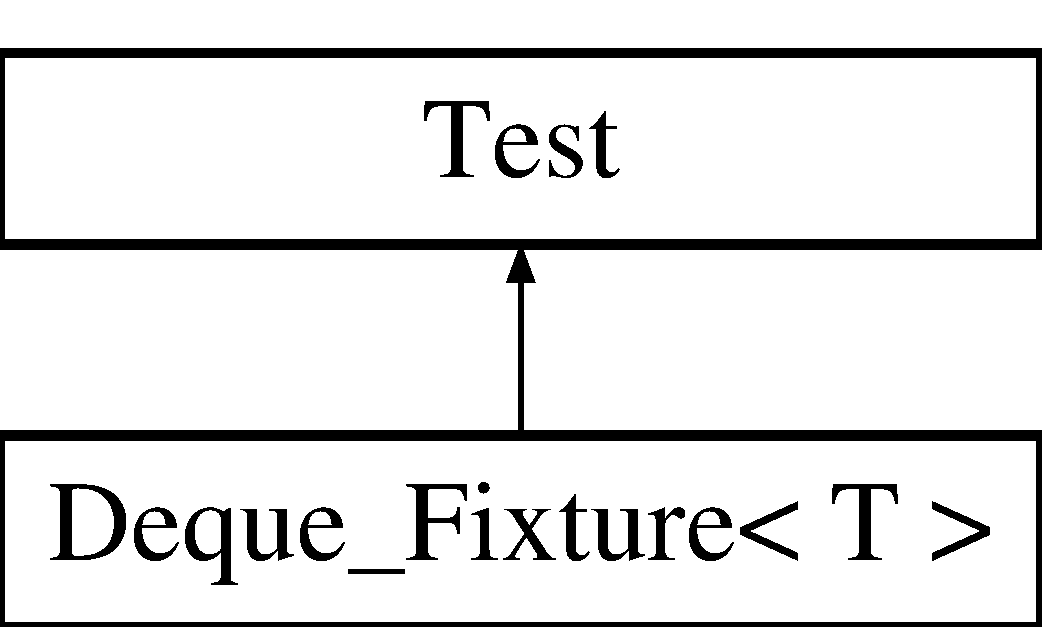
\includegraphics[height=2.000000cm]{structDeque__Fixture}
\end{center}
\end{figure}
\subsection*{Public Types}
\begin{DoxyCompactItemize}
\item 
typedef T \hyperlink{structDeque__Fixture_aff55aebc9f3732e55b5e9afae069a6e7}{deque\-\_\-type}
\item 
typedef deque\-\_\-type\-::value\-\_\-type \hyperlink{structDeque__Fixture_ad3f31d2190bcef2a8809aae173c159e9}{value\-\_\-type}
\item 
typedef deque\-\_\-type\-::size\-\_\-type \hyperlink{structDeque__Fixture_aaf7d8d8eda0003cc8727d9eab7f22086}{size\-\_\-type}
\end{DoxyCompactItemize}


\subsection{Member Typedef Documentation}
\hypertarget{structDeque__Fixture_aff55aebc9f3732e55b5e9afae069a6e7}{\index{Deque\-\_\-\-Fixture@{Deque\-\_\-\-Fixture}!deque\-\_\-type@{deque\-\_\-type}}
\index{deque\-\_\-type@{deque\-\_\-type}!Deque_Fixture@{Deque\-\_\-\-Fixture}}
\subsubsection[{deque\-\_\-type}]{\setlength{\rightskip}{0pt plus 5cm}template$<$typename T $>$ typedef T {\bf Deque\-\_\-\-Fixture}$<$ T $>$\-::{\bf deque\-\_\-type}}}\label{structDeque__Fixture_aff55aebc9f3732e55b5e9afae069a6e7}
\hypertarget{structDeque__Fixture_aaf7d8d8eda0003cc8727d9eab7f22086}{\index{Deque\-\_\-\-Fixture@{Deque\-\_\-\-Fixture}!size\-\_\-type@{size\-\_\-type}}
\index{size\-\_\-type@{size\-\_\-type}!Deque_Fixture@{Deque\-\_\-\-Fixture}}
\subsubsection[{size\-\_\-type}]{\setlength{\rightskip}{0pt plus 5cm}template$<$typename T $>$ typedef deque\-\_\-type\-::size\-\_\-type {\bf Deque\-\_\-\-Fixture}$<$ T $>$\-::{\bf size\-\_\-type}}}\label{structDeque__Fixture_aaf7d8d8eda0003cc8727d9eab7f22086}
\hypertarget{structDeque__Fixture_ad3f31d2190bcef2a8809aae173c159e9}{\index{Deque\-\_\-\-Fixture@{Deque\-\_\-\-Fixture}!value\-\_\-type@{value\-\_\-type}}
\index{value\-\_\-type@{value\-\_\-type}!Deque_Fixture@{Deque\-\_\-\-Fixture}}
\subsubsection[{value\-\_\-type}]{\setlength{\rightskip}{0pt plus 5cm}template$<$typename T $>$ typedef deque\-\_\-type\-::value\-\_\-type {\bf Deque\-\_\-\-Fixture}$<$ T $>$\-::{\bf value\-\_\-type}}}\label{structDeque__Fixture_ad3f31d2190bcef2a8809aae173c159e9}


The documentation for this struct was generated from the following file\-:\begin{DoxyCompactItemize}
\item 
\hyperlink{TestDeque_8c_09_09}{Test\-Deque.\-c++}\end{DoxyCompactItemize}

\hypertarget{classmy__deque_1_1iterator}{\section{my\-\_\-deque$<$ T, A $>$\-:\-:iterator Class Reference}
\label{classmy__deque_1_1iterator}\index{my\-\_\-deque$<$ T, A $>$\-::iterator@{my\-\_\-deque$<$ T, A $>$\-::iterator}}
}


{\ttfamily \#include $<$Deque.\-h$>$}

\subsection*{Public Types}
\begin{DoxyCompactItemize}
\item 
typedef \\*
std\-::bidirectional\-\_\-iterator\-\_\-tag \hyperlink{classmy__deque_1_1iterator_a0479a0f5fbb1adddafb03cd2c9aaef53}{iterator\-\_\-category}
\item 
typedef \hyperlink{classmy__deque_ae9c156c405acc57623a4601ce755596f}{my\-\_\-deque\-::value\-\_\-type} \hyperlink{classmy__deque_1_1iterator_ac6392e82698893d1802ef0407bd36794}{value\-\_\-type}
\item 
typedef \hyperlink{classmy__deque_ac85676cb2492fbc9bbc6f1a30e9d3c73}{my\-\_\-deque\-::difference\-\_\-type} \hyperlink{classmy__deque_1_1iterator_ac5f62e8566ad92478931c2abd9ac6596}{difference\-\_\-type}
\item 
typedef \hyperlink{classmy__deque_a58e82fc365a3b086367479515e1515be}{my\-\_\-deque\-::pointer} \hyperlink{classmy__deque_1_1iterator_add0e1ed49072422b5aa0ef52303fb86e}{pointer}
\item 
typedef \hyperlink{classmy__deque_a4c34c14f397b7676445b37c87003116b}{my\-\_\-deque\-::reference} \hyperlink{classmy__deque_1_1iterator_ae165ee997a9e18330c593789e9899e57}{reference}
\end{DoxyCompactItemize}
\subsection*{Public Member Functions}
\begin{DoxyCompactItemize}
\item 
\hyperlink{classmy__deque_1_1iterator_a3f9e14fe295b2d79df0c1704f5fc51d1}{iterator} (\hyperlink{classmy__deque}{my\-\_\-deque} $\ast$d, \hyperlink{classmy__deque_a61e5e5317fe72a381ce4d45f09544b02}{size\-\_\-type} s)
\item 
\hyperlink{classmy__deque_1_1iterator_ae165ee997a9e18330c593789e9899e57}{reference} \hyperlink{classmy__deque_1_1iterator_a12632f02814bba64ca79f42edc0e1497}{operator$\ast$} () const 
\item 
\hyperlink{classmy__deque_1_1iterator_add0e1ed49072422b5aa0ef52303fb86e}{pointer} \hyperlink{classmy__deque_1_1iterator_a064f5b1faf5a72113083425133de9a41}{operator-\/$>$} () const 
\item 
\hyperlink{classmy__deque_1_1iterator}{iterator} \& \hyperlink{classmy__deque_1_1iterator_ab2a00619614e204eedb184112a56016e}{operator++} ()
\item 
\hyperlink{classmy__deque_1_1iterator}{iterator} \hyperlink{classmy__deque_1_1iterator_a57f6ac4aef7215ca67b6e05eeda29ee4}{operator++} (int)
\item 
\hyperlink{classmy__deque_1_1iterator}{iterator} \& \hyperlink{classmy__deque_1_1iterator_a278cab96c03498e55ba1aa4e05f1538e}{operator-\/-\/} ()
\item 
\hyperlink{classmy__deque_1_1iterator}{iterator} \hyperlink{classmy__deque_1_1iterator_a5bef4b6332aecf7dcda57cee9a1fdc70}{operator-\/-\/} (int)
\item 
\hyperlink{classmy__deque_1_1iterator}{iterator} \& \hyperlink{classmy__deque_1_1iterator_ad17b4f6e8be4d8242ad4572d62beff82}{operator+=} (\hyperlink{classmy__deque_1_1iterator_ac5f62e8566ad92478931c2abd9ac6596}{difference\-\_\-type} d)
\item 
\hyperlink{classmy__deque_1_1iterator}{iterator} \& \hyperlink{classmy__deque_1_1iterator_a13c056d48543734a23a9de09fd652868}{operator-\/=} (\hyperlink{classmy__deque_1_1iterator_ac5f62e8566ad92478931c2abd9ac6596}{difference\-\_\-type} d)
\end{DoxyCompactItemize}
\subsection*{Private Member Functions}
\begin{DoxyCompactItemize}
\item 
bool \hyperlink{classmy__deque_1_1iterator_a4e56b174bbf8c52c58e2f3934be7fc75}{valid} () const 
\end{DoxyCompactItemize}
\subsection*{Private Attributes}
\begin{DoxyCompactItemize}
\item 
\hyperlink{classmy__deque}{my\-\_\-deque} $\ast$ \hyperlink{classmy__deque_1_1iterator_a69df69b162f6a0fb1f6e59bdccb639c4}{\-\_\-d}
\item 
\hyperlink{classmy__deque_a61e5e5317fe72a381ce4d45f09544b02}{size\-\_\-type} \hyperlink{classmy__deque_1_1iterator_a41f01f39f26a404b45742e43c3352917}{\-\_\-index}
\end{DoxyCompactItemize}
\subsection*{Friends}
\begin{DoxyCompactItemize}
\item 
bool \hyperlink{classmy__deque_1_1iterator_a27d0df37bd079bf4e62faa0b468b060c}{operator==} (const \hyperlink{classmy__deque_1_1iterator}{iterator} \&lhs, const \hyperlink{classmy__deque_1_1iterator}{iterator} \&rhs)
\item 
bool \hyperlink{classmy__deque_1_1iterator_aad2b3926ed1e2db6f22ca3117766181b}{operator!=} (const \hyperlink{classmy__deque_1_1iterator}{iterator} \&lhs, const \hyperlink{classmy__deque_1_1iterator}{iterator} \&rhs)
\item 
\hyperlink{classmy__deque_1_1iterator}{iterator} \hyperlink{classmy__deque_1_1iterator_aaf128f38c16b5a8284f51a9c69f6fd77}{operator+} (\hyperlink{classmy__deque_1_1iterator}{iterator} lhs, \hyperlink{classmy__deque_1_1iterator_ac5f62e8566ad92478931c2abd9ac6596}{difference\-\_\-type} rhs)
\item 
\hyperlink{classmy__deque_1_1iterator}{iterator} \hyperlink{classmy__deque_1_1iterator_ab8892736ecb2ffe5f6b9ac9b9dbb60c0}{operator-\/} (\hyperlink{classmy__deque_1_1iterator}{iterator} lhs, \hyperlink{classmy__deque_1_1iterator_ac5f62e8566ad92478931c2abd9ac6596}{difference\-\_\-type} rhs)
\end{DoxyCompactItemize}


\subsection{Member Typedef Documentation}
\hypertarget{classmy__deque_1_1iterator_ac5f62e8566ad92478931c2abd9ac6596}{\index{my\-\_\-deque\-::iterator@{my\-\_\-deque\-::iterator}!difference\-\_\-type@{difference\-\_\-type}}
\index{difference\-\_\-type@{difference\-\_\-type}!my_deque::iterator@{my\-\_\-deque\-::iterator}}
\subsubsection[{difference\-\_\-type}]{\setlength{\rightskip}{0pt plus 5cm}template$<$typename T , typename A  = std\-::allocator$<$\-T$>$$>$ typedef {\bf my\-\_\-deque\-::difference\-\_\-type} {\bf my\-\_\-deque}$<$ T, A $>$\-::{\bf iterator\-::difference\-\_\-type}}}\label{classmy__deque_1_1iterator_ac5f62e8566ad92478931c2abd9ac6596}
\hypertarget{classmy__deque_1_1iterator_a0479a0f5fbb1adddafb03cd2c9aaef53}{\index{my\-\_\-deque\-::iterator@{my\-\_\-deque\-::iterator}!iterator\-\_\-category@{iterator\-\_\-category}}
\index{iterator\-\_\-category@{iterator\-\_\-category}!my_deque::iterator@{my\-\_\-deque\-::iterator}}
\subsubsection[{iterator\-\_\-category}]{\setlength{\rightskip}{0pt plus 5cm}template$<$typename T , typename A  = std\-::allocator$<$\-T$>$$>$ typedef std\-::bidirectional\-\_\-iterator\-\_\-tag {\bf my\-\_\-deque}$<$ T, A $>$\-::{\bf iterator\-::iterator\-\_\-category}}}\label{classmy__deque_1_1iterator_a0479a0f5fbb1adddafb03cd2c9aaef53}
\hypertarget{classmy__deque_1_1iterator_add0e1ed49072422b5aa0ef52303fb86e}{\index{my\-\_\-deque\-::iterator@{my\-\_\-deque\-::iterator}!pointer@{pointer}}
\index{pointer@{pointer}!my_deque::iterator@{my\-\_\-deque\-::iterator}}
\subsubsection[{pointer}]{\setlength{\rightskip}{0pt plus 5cm}template$<$typename T , typename A  = std\-::allocator$<$\-T$>$$>$ typedef {\bf my\-\_\-deque\-::pointer} {\bf my\-\_\-deque}$<$ T, A $>$\-::{\bf iterator\-::pointer}}}\label{classmy__deque_1_1iterator_add0e1ed49072422b5aa0ef52303fb86e}
\hypertarget{classmy__deque_1_1iterator_ae165ee997a9e18330c593789e9899e57}{\index{my\-\_\-deque\-::iterator@{my\-\_\-deque\-::iterator}!reference@{reference}}
\index{reference@{reference}!my_deque::iterator@{my\-\_\-deque\-::iterator}}
\subsubsection[{reference}]{\setlength{\rightskip}{0pt plus 5cm}template$<$typename T , typename A  = std\-::allocator$<$\-T$>$$>$ typedef {\bf my\-\_\-deque\-::reference} {\bf my\-\_\-deque}$<$ T, A $>$\-::{\bf iterator\-::reference}}}\label{classmy__deque_1_1iterator_ae165ee997a9e18330c593789e9899e57}
\hypertarget{classmy__deque_1_1iterator_ac6392e82698893d1802ef0407bd36794}{\index{my\-\_\-deque\-::iterator@{my\-\_\-deque\-::iterator}!value\-\_\-type@{value\-\_\-type}}
\index{value\-\_\-type@{value\-\_\-type}!my_deque::iterator@{my\-\_\-deque\-::iterator}}
\subsubsection[{value\-\_\-type}]{\setlength{\rightskip}{0pt plus 5cm}template$<$typename T , typename A  = std\-::allocator$<$\-T$>$$>$ typedef {\bf my\-\_\-deque\-::value\-\_\-type} {\bf my\-\_\-deque}$<$ T, A $>$\-::{\bf iterator\-::value\-\_\-type}}}\label{classmy__deque_1_1iterator_ac6392e82698893d1802ef0407bd36794}


\subsection{Constructor \& Destructor Documentation}
\hypertarget{classmy__deque_1_1iterator_a3f9e14fe295b2d79df0c1704f5fc51d1}{\index{my\-\_\-deque\-::iterator@{my\-\_\-deque\-::iterator}!iterator@{iterator}}
\index{iterator@{iterator}!my_deque::iterator@{my\-\_\-deque\-::iterator}}
\subsubsection[{iterator}]{\setlength{\rightskip}{0pt plus 5cm}template$<$typename T , typename A  = std\-::allocator$<$\-T$>$$>$ {\bf my\-\_\-deque}$<$ T, A $>$\-::iterator\-::iterator (
\begin{DoxyParamCaption}
\item[{{\bf my\-\_\-deque} $\ast$}]{d, }
\item[{{\bf size\-\_\-type}}]{s}
\end{DoxyParamCaption}
)\hspace{0.3cm}{\ttfamily [inline]}}}\label{classmy__deque_1_1iterator_a3f9e14fe295b2d79df0c1704f5fc51d1}
iterator constructor 
\begin{DoxyParams}{Parameters}
{\em my\-\_\-deque$\ast$} & d \\
\hline
{\em size\-\_\-type} & s \\
\hline
\end{DoxyParams}
\begin{DoxyReturn}{Returns}
iterator pointing to \hyperlink{classmy__deque}{my\-\_\-deque} d at position s 
\end{DoxyReturn}


\subsection{Member Function Documentation}
\hypertarget{classmy__deque_1_1iterator_a12632f02814bba64ca79f42edc0e1497}{\index{my\-\_\-deque\-::iterator@{my\-\_\-deque\-::iterator}!operator$\ast$@{operator$\ast$}}
\index{operator$\ast$@{operator$\ast$}!my_deque::iterator@{my\-\_\-deque\-::iterator}}
\subsubsection[{operator$\ast$}]{\setlength{\rightskip}{0pt plus 5cm}template$<$typename T , typename A  = std\-::allocator$<$\-T$>$$>$ {\bf reference} {\bf my\-\_\-deque}$<$ T, A $>$\-::iterator\-::operator$\ast$ (
\begin{DoxyParamCaption}
{}
\end{DoxyParamCaption}
) const\hspace{0.3cm}{\ttfamily [inline]}}}\label{classmy__deque_1_1iterator_a12632f02814bba64ca79f42edc0e1497}
\begin{DoxyReturn}{Returns}
reference at \-\_\-d\mbox{[}\-\_\-index\mbox{]} 
\end{DoxyReturn}
\hypertarget{classmy__deque_1_1iterator_ab2a00619614e204eedb184112a56016e}{\index{my\-\_\-deque\-::iterator@{my\-\_\-deque\-::iterator}!operator++@{operator++}}
\index{operator++@{operator++}!my_deque::iterator@{my\-\_\-deque\-::iterator}}
\subsubsection[{operator++}]{\setlength{\rightskip}{0pt plus 5cm}template$<$typename T , typename A  = std\-::allocator$<$\-T$>$$>$ {\bf iterator}\& {\bf my\-\_\-deque}$<$ T, A $>$\-::iterator\-::operator++ (
\begin{DoxyParamCaption}
{}
\end{DoxyParamCaption}
)\hspace{0.3cm}{\ttfamily [inline]}}}\label{classmy__deque_1_1iterator_ab2a00619614e204eedb184112a56016e}
prefix ++ \begin{DoxyReturn}{Returns}
iterator incremented 
\end{DoxyReturn}
\hypertarget{classmy__deque_1_1iterator_a57f6ac4aef7215ca67b6e05eeda29ee4}{\index{my\-\_\-deque\-::iterator@{my\-\_\-deque\-::iterator}!operator++@{operator++}}
\index{operator++@{operator++}!my_deque::iterator@{my\-\_\-deque\-::iterator}}
\subsubsection[{operator++}]{\setlength{\rightskip}{0pt plus 5cm}template$<$typename T , typename A  = std\-::allocator$<$\-T$>$$>$ {\bf iterator} {\bf my\-\_\-deque}$<$ T, A $>$\-::iterator\-::operator++ (
\begin{DoxyParamCaption}
\item[{int}]{}
\end{DoxyParamCaption}
)\hspace{0.3cm}{\ttfamily [inline]}}}\label{classmy__deque_1_1iterator_a57f6ac4aef7215ca67b6e05eeda29ee4}
postfix ++ 
\begin{DoxyParams}{Parameters}
{\em int} & \\
\hline
\end{DoxyParams}
\begin{DoxyReturn}{Returns}
iterator pointing to original value with internal value decremented 
\end{DoxyReturn}
\hypertarget{classmy__deque_1_1iterator_ad17b4f6e8be4d8242ad4572d62beff82}{\index{my\-\_\-deque\-::iterator@{my\-\_\-deque\-::iterator}!operator+=@{operator+=}}
\index{operator+=@{operator+=}!my_deque::iterator@{my\-\_\-deque\-::iterator}}
\subsubsection[{operator+=}]{\setlength{\rightskip}{0pt plus 5cm}template$<$typename T , typename A  = std\-::allocator$<$\-T$>$$>$ {\bf iterator}\& {\bf my\-\_\-deque}$<$ T, A $>$\-::iterator\-::operator+= (
\begin{DoxyParamCaption}
\item[{{\bf difference\-\_\-type}}]{d}
\end{DoxyParamCaption}
)\hspace{0.3cm}{\ttfamily [inline]}}}\label{classmy__deque_1_1iterator_ad17b4f6e8be4d8242ad4572d62beff82}

\begin{DoxyParams}{Parameters}
{\em difference\-\_\-type} & d \\
\hline
\end{DoxyParams}
\begin{DoxyReturn}{Returns}
iterator to current position + d 
\end{DoxyReturn}
\hypertarget{classmy__deque_1_1iterator_a278cab96c03498e55ba1aa4e05f1538e}{\index{my\-\_\-deque\-::iterator@{my\-\_\-deque\-::iterator}!operator-\/-\/@{operator-\/-\/}}
\index{operator-\/-\/@{operator-\/-\/}!my_deque::iterator@{my\-\_\-deque\-::iterator}}
\subsubsection[{operator-\/-\/}]{\setlength{\rightskip}{0pt plus 5cm}template$<$typename T , typename A  = std\-::allocator$<$\-T$>$$>$ {\bf iterator}\& {\bf my\-\_\-deque}$<$ T, A $>$\-::iterator\-::operator-\/-\/ (
\begin{DoxyParamCaption}
{}
\end{DoxyParamCaption}
)\hspace{0.3cm}{\ttfamily [inline]}}}\label{classmy__deque_1_1iterator_a278cab96c03498e55ba1aa4e05f1538e}
prefix -- \begin{DoxyReturn}{Returns}
iterator decremented 
\end{DoxyReturn}
\hypertarget{classmy__deque_1_1iterator_a5bef4b6332aecf7dcda57cee9a1fdc70}{\index{my\-\_\-deque\-::iterator@{my\-\_\-deque\-::iterator}!operator-\/-\/@{operator-\/-\/}}
\index{operator-\/-\/@{operator-\/-\/}!my_deque::iterator@{my\-\_\-deque\-::iterator}}
\subsubsection[{operator-\/-\/}]{\setlength{\rightskip}{0pt plus 5cm}template$<$typename T , typename A  = std\-::allocator$<$\-T$>$$>$ {\bf iterator} {\bf my\-\_\-deque}$<$ T, A $>$\-::iterator\-::operator-\/-\/ (
\begin{DoxyParamCaption}
\item[{int}]{}
\end{DoxyParamCaption}
)\hspace{0.3cm}{\ttfamily [inline]}}}\label{classmy__deque_1_1iterator_a5bef4b6332aecf7dcda57cee9a1fdc70}
postfix -- 
\begin{DoxyParams}{Parameters}
{\em int} & \\
\hline
\end{DoxyParams}
\begin{DoxyReturn}{Returns}
iterator pointing to original value with internal value decremented 
\end{DoxyReturn}
\hypertarget{classmy__deque_1_1iterator_a13c056d48543734a23a9de09fd652868}{\index{my\-\_\-deque\-::iterator@{my\-\_\-deque\-::iterator}!operator-\/=@{operator-\/=}}
\index{operator-\/=@{operator-\/=}!my_deque::iterator@{my\-\_\-deque\-::iterator}}
\subsubsection[{operator-\/=}]{\setlength{\rightskip}{0pt plus 5cm}template$<$typename T , typename A  = std\-::allocator$<$\-T$>$$>$ {\bf iterator}\& {\bf my\-\_\-deque}$<$ T, A $>$\-::iterator\-::operator-\/= (
\begin{DoxyParamCaption}
\item[{{\bf difference\-\_\-type}}]{d}
\end{DoxyParamCaption}
)\hspace{0.3cm}{\ttfamily [inline]}}}\label{classmy__deque_1_1iterator_a13c056d48543734a23a9de09fd652868}

\begin{DoxyParams}{Parameters}
{\em difference\-\_\-type} & d \\
\hline
\end{DoxyParams}
\begin{DoxyReturn}{Returns}
iterator to current position -\/ d 
\end{DoxyReturn}
\hypertarget{classmy__deque_1_1iterator_a064f5b1faf5a72113083425133de9a41}{\index{my\-\_\-deque\-::iterator@{my\-\_\-deque\-::iterator}!operator-\/$>$@{operator-\/$>$}}
\index{operator-\/$>$@{operator-\/$>$}!my_deque::iterator@{my\-\_\-deque\-::iterator}}
\subsubsection[{operator-\/$>$}]{\setlength{\rightskip}{0pt plus 5cm}template$<$typename T , typename A  = std\-::allocator$<$\-T$>$$>$ {\bf pointer} {\bf my\-\_\-deque}$<$ T, A $>$\-::iterator\-::operator-\/$>$ (
\begin{DoxyParamCaption}
{}
\end{DoxyParamCaption}
) const\hspace{0.3cm}{\ttfamily [inline]}}}\label{classmy__deque_1_1iterator_a064f5b1faf5a72113083425133de9a41}
\begin{DoxyReturn}{Returns}
pointer to this object which can be dereferenced as an rvalue 
\end{DoxyReturn}
\hypertarget{classmy__deque_1_1iterator_a4e56b174bbf8c52c58e2f3934be7fc75}{\index{my\-\_\-deque\-::iterator@{my\-\_\-deque\-::iterator}!valid@{valid}}
\index{valid@{valid}!my_deque::iterator@{my\-\_\-deque\-::iterator}}
\subsubsection[{valid}]{\setlength{\rightskip}{0pt plus 5cm}template$<$typename T , typename A  = std\-::allocator$<$\-T$>$$>$ bool {\bf my\-\_\-deque}$<$ T, A $>$\-::iterator\-::valid (
\begin{DoxyParamCaption}
{}
\end{DoxyParamCaption}
) const\hspace{0.3cm}{\ttfamily [inline]}, {\ttfamily [private]}}}\label{classmy__deque_1_1iterator_a4e56b174bbf8c52c58e2f3934be7fc75}


\subsection{Friends And Related Function Documentation}
\hypertarget{classmy__deque_1_1iterator_aad2b3926ed1e2db6f22ca3117766181b}{\index{my\-\_\-deque\-::iterator@{my\-\_\-deque\-::iterator}!operator!=@{operator!=}}
\index{operator!=@{operator!=}!my_deque::iterator@{my\-\_\-deque\-::iterator}}
\subsubsection[{operator!=}]{\setlength{\rightskip}{0pt plus 5cm}template$<$typename T , typename A  = std\-::allocator$<$\-T$>$$>$ bool operator!= (
\begin{DoxyParamCaption}
\item[{const {\bf iterator} \&}]{lhs, }
\item[{const {\bf iterator} \&}]{rhs}
\end{DoxyParamCaption}
)\hspace{0.3cm}{\ttfamily [friend]}}}\label{classmy__deque_1_1iterator_aad2b3926ed1e2db6f22ca3117766181b}

\begin{DoxyParams}{Parameters}
{\em iterator} & lhs \\
\hline
{\em difference\-\_\-type} & rhs \\
\hline
\end{DoxyParams}
\begin{DoxyReturn}{Returns}
true if lhs!=rhs, false otherwise 
\end{DoxyReturn}
\hypertarget{classmy__deque_1_1iterator_aaf128f38c16b5a8284f51a9c69f6fd77}{\index{my\-\_\-deque\-::iterator@{my\-\_\-deque\-::iterator}!operator+@{operator+}}
\index{operator+@{operator+}!my_deque::iterator@{my\-\_\-deque\-::iterator}}
\subsubsection[{operator+}]{\setlength{\rightskip}{0pt plus 5cm}template$<$typename T , typename A  = std\-::allocator$<$\-T$>$$>$ {\bf iterator} operator+ (
\begin{DoxyParamCaption}
\item[{{\bf iterator}}]{lhs, }
\item[{{\bf difference\-\_\-type}}]{rhs}
\end{DoxyParamCaption}
)\hspace{0.3cm}{\ttfamily [friend]}}}\label{classmy__deque_1_1iterator_aaf128f38c16b5a8284f51a9c69f6fd77}

\begin{DoxyParams}{Parameters}
{\em iterator} & lhs \\
\hline
{\em difference\-\_\-type} & rhs \\
\hline
\end{DoxyParams}
\begin{DoxyReturn}{Returns}
iterator lhs+rhs 
\end{DoxyReturn}
\hypertarget{classmy__deque_1_1iterator_ab8892736ecb2ffe5f6b9ac9b9dbb60c0}{\index{my\-\_\-deque\-::iterator@{my\-\_\-deque\-::iterator}!operator-\/@{operator-\/}}
\index{operator-\/@{operator-\/}!my_deque::iterator@{my\-\_\-deque\-::iterator}}
\subsubsection[{operator-\/}]{\setlength{\rightskip}{0pt plus 5cm}template$<$typename T , typename A  = std\-::allocator$<$\-T$>$$>$ {\bf iterator} operator-\/ (
\begin{DoxyParamCaption}
\item[{{\bf iterator}}]{lhs, }
\item[{{\bf difference\-\_\-type}}]{rhs}
\end{DoxyParamCaption}
)\hspace{0.3cm}{\ttfamily [friend]}}}\label{classmy__deque_1_1iterator_ab8892736ecb2ffe5f6b9ac9b9dbb60c0}

\begin{DoxyParams}{Parameters}
{\em iterator} & lhs \\
\hline
{\em difference\-\_\-type} & rhs \\
\hline
\end{DoxyParams}
\begin{DoxyReturn}{Returns}
iterator lhs-\/rhs 
\end{DoxyReturn}
\hypertarget{classmy__deque_1_1iterator_a27d0df37bd079bf4e62faa0b468b060c}{\index{my\-\_\-deque\-::iterator@{my\-\_\-deque\-::iterator}!operator==@{operator==}}
\index{operator==@{operator==}!my_deque::iterator@{my\-\_\-deque\-::iterator}}
\subsubsection[{operator==}]{\setlength{\rightskip}{0pt plus 5cm}template$<$typename T , typename A  = std\-::allocator$<$\-T$>$$>$ bool operator== (
\begin{DoxyParamCaption}
\item[{const {\bf iterator} \&}]{lhs, }
\item[{const {\bf iterator} \&}]{rhs}
\end{DoxyParamCaption}
)\hspace{0.3cm}{\ttfamily [friend]}}}\label{classmy__deque_1_1iterator_a27d0df37bd079bf4e62faa0b468b060c}

\begin{DoxyParams}{Parameters}
{\em iterator} & lhs \\
\hline
{\em difference\-\_\-type} & rhs \\
\hline
\end{DoxyParams}
\begin{DoxyReturn}{Returns}
true if lhs==rhs, false otherwise 
\end{DoxyReturn}


\subsection{Member Data Documentation}
\hypertarget{classmy__deque_1_1iterator_a69df69b162f6a0fb1f6e59bdccb639c4}{\index{my\-\_\-deque\-::iterator@{my\-\_\-deque\-::iterator}!\-\_\-d@{\-\_\-d}}
\index{\-\_\-d@{\-\_\-d}!my_deque::iterator@{my\-\_\-deque\-::iterator}}
\subsubsection[{\-\_\-d}]{\setlength{\rightskip}{0pt plus 5cm}template$<$typename T , typename A  = std\-::allocator$<$\-T$>$$>$ {\bf my\-\_\-deque}$\ast$ {\bf my\-\_\-deque}$<$ T, A $>$\-::iterator\-::\-\_\-d\hspace{0.3cm}{\ttfamily [private]}}}\label{classmy__deque_1_1iterator_a69df69b162f6a0fb1f6e59bdccb639c4}
\hypertarget{classmy__deque_1_1iterator_a41f01f39f26a404b45742e43c3352917}{\index{my\-\_\-deque\-::iterator@{my\-\_\-deque\-::iterator}!\-\_\-index@{\-\_\-index}}
\index{\-\_\-index@{\-\_\-index}!my_deque::iterator@{my\-\_\-deque\-::iterator}}
\subsubsection[{\-\_\-index}]{\setlength{\rightskip}{0pt plus 5cm}template$<$typename T , typename A  = std\-::allocator$<$\-T$>$$>$ {\bf size\-\_\-type} {\bf my\-\_\-deque}$<$ T, A $>$\-::iterator\-::\-\_\-index\hspace{0.3cm}{\ttfamily [private]}}}\label{classmy__deque_1_1iterator_a41f01f39f26a404b45742e43c3352917}


The documentation for this class was generated from the following file\-:\begin{DoxyCompactItemize}
\item 
\hyperlink{Deque_8h}{Deque.\-h}\end{DoxyCompactItemize}

\hypertarget{classmy__deque}{\section{my\-\_\-deque$<$ T, A $>$ Class Template Reference}
\label{classmy__deque}\index{my\-\_\-deque$<$ T, A $>$@{my\-\_\-deque$<$ T, A $>$}}
}


{\ttfamily \#include $<$Deque.\-h$>$}

\subsection*{Classes}
\begin{DoxyCompactItemize}
\item 
class \hyperlink{classmy__deque_1_1const__iterator}{const\-\_\-iterator}
\item 
class \hyperlink{classmy__deque_1_1iterator}{iterator}
\end{DoxyCompactItemize}
\subsection*{Public Types}
\begin{DoxyCompactItemize}
\item 
typedef A \hyperlink{classmy__deque_a34236f0fef930decd11dc683f40a38be}{allocator\-\_\-type}
\item 
typedef allocator\-\_\-type\-::value\-\_\-type \hyperlink{classmy__deque_ae9c156c405acc57623a4601ce755596f}{value\-\_\-type}
\item 
typedef allocator\-\_\-type\-::size\-\_\-type \hyperlink{classmy__deque_a61e5e5317fe72a381ce4d45f09544b02}{size\-\_\-type}
\item 
typedef \\*
allocator\-\_\-type\-::difference\-\_\-type \hyperlink{classmy__deque_ac85676cb2492fbc9bbc6f1a30e9d3c73}{difference\-\_\-type}
\item 
typedef allocator\-\_\-type\-::pointer \hyperlink{classmy__deque_a58e82fc365a3b086367479515e1515be}{pointer}
\item 
typedef \\*
allocator\-\_\-type\-::const\-\_\-pointer \hyperlink{classmy__deque_a8fea5edeb2b2cf3dd1246dc3abf9b71b}{const\-\_\-pointer}
\item 
typedef allocator\-\_\-type\-::reference \hyperlink{classmy__deque_a4c34c14f397b7676445b37c87003116b}{reference}
\item 
typedef \\*
allocator\-\_\-type\-::const\-\_\-reference \hyperlink{classmy__deque_ad50d8b378580088cf77fa43f0640e49c}{const\-\_\-reference}
\item 
typedef A\-::template rebind\\*
$<$ \hyperlink{classmy__deque_a58e82fc365a3b086367479515e1515be}{pointer} $>$\-::other \hyperlink{classmy__deque_a1a55c016646bba79086d90d3cccde143}{B}
\end{DoxyCompactItemize}
\subsection*{Public Member Functions}
\begin{DoxyCompactItemize}
\item 
\hyperlink{classmy__deque_ad2ac9d80048c55fcc045d2861c73aa1a}{my\-\_\-deque} (const \hyperlink{classmy__deque_a34236f0fef930decd11dc683f40a38be}{allocator\-\_\-type} \&a=\hyperlink{classmy__deque_a34236f0fef930decd11dc683f40a38be}{allocator\-\_\-type}())
\item 
\hyperlink{classmy__deque_aeaf4c625438497a7cd6a670da6c2c08b}{my\-\_\-deque} (\hyperlink{classmy__deque_a61e5e5317fe72a381ce4d45f09544b02}{size\-\_\-type} s, \hyperlink{classmy__deque_ad50d8b378580088cf77fa43f0640e49c}{const\-\_\-reference} v=\hyperlink{classmy__deque_ae9c156c405acc57623a4601ce755596f}{value\-\_\-type}(), const \hyperlink{classmy__deque_a34236f0fef930decd11dc683f40a38be}{allocator\-\_\-type} \&a=\hyperlink{classmy__deque_a34236f0fef930decd11dc683f40a38be}{allocator\-\_\-type}())
\item 
\hyperlink{classmy__deque_a59015bc46e6096555d631d69dc8fd7e7}{my\-\_\-deque} (const \hyperlink{classmy__deque}{my\-\_\-deque} \&that)
\item 
\hyperlink{classmy__deque_ae22194ee436865a59a7475c339a9c1ca}{$\sim$my\-\_\-deque} ()
\item 
\hyperlink{classmy__deque}{my\-\_\-deque} \& \hyperlink{classmy__deque_aaa103f2058854bb98e500de6305b1564}{operator=} (const \hyperlink{classmy__deque}{my\-\_\-deque} \&rhs)
\item 
\hyperlink{classmy__deque_a4c34c14f397b7676445b37c87003116b}{reference} \hyperlink{classmy__deque_a489b77decf4d424f43092e194d69444f}{operator\mbox{[}$\,$\mbox{]}} (\hyperlink{classmy__deque_a61e5e5317fe72a381ce4d45f09544b02}{size\-\_\-type} index)
\item 
\hyperlink{classmy__deque_ad50d8b378580088cf77fa43f0640e49c}{const\-\_\-reference} \hyperlink{classmy__deque_ad79fcd9e94dfc5566e1cd0ce606cf208}{operator\mbox{[}$\,$\mbox{]}} (\hyperlink{classmy__deque_a61e5e5317fe72a381ce4d45f09544b02}{size\-\_\-type} index) const 
\item 
\hyperlink{classmy__deque_a4c34c14f397b7676445b37c87003116b}{reference} \hyperlink{classmy__deque_a75106748e6ff8735e40560e7335bd500}{at} (\hyperlink{classmy__deque_a61e5e5317fe72a381ce4d45f09544b02}{size\-\_\-type} index)
\item 
\hyperlink{classmy__deque_ad50d8b378580088cf77fa43f0640e49c}{const\-\_\-reference} \hyperlink{classmy__deque_a9642816a10e6a6ee1f8a5367987b8ee8}{at} (\hyperlink{classmy__deque_a61e5e5317fe72a381ce4d45f09544b02}{size\-\_\-type} index) const 
\item 
\hyperlink{classmy__deque_a4c34c14f397b7676445b37c87003116b}{reference} \hyperlink{classmy__deque_a1d9aadb5bedc29da86d4323587cd5e4d}{back} ()
\item 
\hyperlink{classmy__deque_ad50d8b378580088cf77fa43f0640e49c}{const\-\_\-reference} \hyperlink{classmy__deque_ac273f9574a95af619b9f0dcc0d2e89d0}{back} () const 
\item 
\hyperlink{classmy__deque_1_1iterator}{iterator} \hyperlink{classmy__deque_aef8cac69d47cb1c274896b82ba8f453a}{begin} ()
\item 
\hyperlink{classmy__deque_1_1const__iterator}{const\-\_\-iterator} \hyperlink{classmy__deque_a8612539eff4ee446f85ffb30abf91a69}{begin} () const 
\item 
\hyperlink{classmy__deque_a61e5e5317fe72a381ce4d45f09544b02}{size\-\_\-type} \hyperlink{classmy__deque_a6402ba96543ef0e121dc72e4429b048f}{capacity} () const 
\item 
void \hyperlink{classmy__deque_aa29f90c63cde532f5fc169e8e66b514c}{clear} ()
\item 
bool \hyperlink{classmy__deque_a2b4f029c47afbdbf057639c5a6816d6c}{empty} () const 
\item 
\hyperlink{classmy__deque_1_1iterator}{iterator} \hyperlink{classmy__deque_a2576ee71790ebe55ac4200c506540bb5}{end} ()
\item 
\hyperlink{classmy__deque_1_1const__iterator}{const\-\_\-iterator} \hyperlink{classmy__deque_af465c3f8483634e4e656d90f8d0d88fb}{end} () const 
\item 
\hyperlink{classmy__deque_1_1iterator}{iterator} \hyperlink{classmy__deque_a08d9ba017ff4874a682d1cb58dd46cb7}{erase} (\hyperlink{classmy__deque_1_1iterator}{iterator} it)
\item 
\hyperlink{classmy__deque_a4c34c14f397b7676445b37c87003116b}{reference} \hyperlink{classmy__deque_a0eae28af0ffdd813d1f94f57d393fdf8}{front} ()
\item 
\hyperlink{classmy__deque_ad50d8b378580088cf77fa43f0640e49c}{const\-\_\-reference} \hyperlink{classmy__deque_a0f1239043b7339b8237a0c8bc663be6b}{front} () const 
\item 
\hyperlink{classmy__deque_1_1iterator}{iterator} \hyperlink{classmy__deque_acce29d6597777d85a6745bd937d9b353}{insert} (\hyperlink{classmy__deque_1_1iterator}{iterator} it, \hyperlink{classmy__deque_ad50d8b378580088cf77fa43f0640e49c}{const\-\_\-reference} val)
\item 
void \hyperlink{classmy__deque_a63cc9691ee90701693e948246311c498}{pop\-\_\-back} ()
\item 
void \hyperlink{classmy__deque_a85c322cdc4f629e44abdcf369fdd3dab}{pop\-\_\-front} ()
\item 
void \hyperlink{classmy__deque_a15867a8b57c321dcc8ebb4cfa785d7ca}{push\-\_\-back} (\hyperlink{classmy__deque_ad50d8b378580088cf77fa43f0640e49c}{const\-\_\-reference} v)
\item 
void \hyperlink{classmy__deque_af8d66a7ed1fd51476ec785228ac76996}{push\-\_\-front} (\hyperlink{classmy__deque_ad50d8b378580088cf77fa43f0640e49c}{const\-\_\-reference} v)
\item 
void \hyperlink{classmy__deque_a80369f549dcd0a2ea9bc086fc97c8e25}{resize} (\hyperlink{classmy__deque_a61e5e5317fe72a381ce4d45f09544b02}{size\-\_\-type} s, \hyperlink{classmy__deque_ad50d8b378580088cf77fa43f0640e49c}{const\-\_\-reference} v=\hyperlink{classmy__deque_ae9c156c405acc57623a4601ce755596f}{value\-\_\-type}())
\item 
void \hyperlink{classmy__deque_ae9b535414a0575bc30f8a90b894adfac}{reserve} (\hyperlink{classmy__deque_a61e5e5317fe72a381ce4d45f09544b02}{size\-\_\-type} c)
\item 
\hyperlink{classmy__deque_a61e5e5317fe72a381ce4d45f09544b02}{size\-\_\-type} \hyperlink{classmy__deque_a3100498f22d2dfa480b141f8ef7990ca}{size} () const 
\item 
void \hyperlink{classmy__deque_a22e1c253ac010e4327c87293b6cfbe5c}{swap} (\hyperlink{classmy__deque}{my\-\_\-deque} \&rhs)
\end{DoxyCompactItemize}
\subsection*{Private Member Functions}
\begin{DoxyCompactItemize}
\item 
bool \hyperlink{classmy__deque_ac48856ffa58fe0d4d21852c503d7ff73}{valid} () const 
\end{DoxyCompactItemize}
\subsection*{Private Attributes}
\begin{DoxyCompactItemize}
\item 
\hyperlink{classmy__deque_a34236f0fef930decd11dc683f40a38be}{allocator\-\_\-type} \hyperlink{classmy__deque_ab2ba2e14114a27b2f91e47dfccabc639}{\-\_\-a}
\item 
int \hyperlink{classmy__deque_a27647dca34c708d1b4705ede6d46fd7e}{O\-U\-T\-E\-R\-\_\-\-S\-I\-Z\-E}
\item 
\hyperlink{classmy__deque_a1a55c016646bba79086d90d3cccde143}{B} \hyperlink{classmy__deque_aff09be5225ab5c67ce40d4876a3afbe7}{\-\_\-balloc}
\item 
\hyperlink{classmy__deque_a58e82fc365a3b086367479515e1515be}{pointer} $\ast$ \hyperlink{classmy__deque_afe69687aa94aa63dbb23e147a90db3d1}{outer\-\_\-b}
\item 
\hyperlink{classmy__deque_a58e82fc365a3b086367479515e1515be}{pointer} $\ast$ \hyperlink{classmy__deque_a4d7496e28dd1a7bda7df4c6861b1f5c1}{outer\-\_\-e}
\item 
\hyperlink{classmy__deque_a58e82fc365a3b086367479515e1515be}{pointer} \hyperlink{classmy__deque_abb765edbf3d947df440a760c5e1eb810}{\-\_\-bstart}
\item 
\hyperlink{classmy__deque_a58e82fc365a3b086367479515e1515be}{pointer} \hyperlink{classmy__deque_ae0e648a3abb9594093b50eaaf09d1e0d}{\-\_\-estart}
\item 
\hyperlink{classmy__deque_a58e82fc365a3b086367479515e1515be}{pointer} \hyperlink{classmy__deque_aaa73de3a597f551851ec4a79c7100dac}{\-\_\-b}
\item 
\hyperlink{classmy__deque_a58e82fc365a3b086367479515e1515be}{pointer} \hyperlink{classmy__deque_aa9adebd4257de224e119b91ef209abca}{\-\_\-e}
\item 
\hyperlink{classmy__deque_a58e82fc365a3b086367479515e1515be}{pointer} \hyperlink{classmy__deque_a3d540bafe793c6ae6ceee0bd78d59a9c}{\-\_\-l}
\item 
int \hyperlink{classmy__deque_a9d27e92833c2e24410dae3b329ebc5da}{\-\_\-size}
\item 
int \hyperlink{classmy__deque_a8f70b94005db4d4780bfd0947568c730}{\-\_\-offset}
\end{DoxyCompactItemize}
\subsection*{Friends}
\begin{DoxyCompactItemize}
\item 
bool \hyperlink{classmy__deque_aca1e37552707f9d7710a6af82cf1262e}{operator==} (const \hyperlink{classmy__deque}{my\-\_\-deque} \&lhs, const \hyperlink{classmy__deque}{my\-\_\-deque} \&rhs)
\item 
bool \hyperlink{classmy__deque_abd32df1d76a0ab0c1519f65cc4fa1363}{operator$<$} (const \hyperlink{classmy__deque}{my\-\_\-deque} \&lhs, const \hyperlink{classmy__deque}{my\-\_\-deque} \&rhs)
\end{DoxyCompactItemize}


\subsection{Member Typedef Documentation}
\hypertarget{classmy__deque_a34236f0fef930decd11dc683f40a38be}{\index{my\-\_\-deque@{my\-\_\-deque}!allocator\-\_\-type@{allocator\-\_\-type}}
\index{allocator\-\_\-type@{allocator\-\_\-type}!my_deque@{my\-\_\-deque}}
\subsubsection[{allocator\-\_\-type}]{\setlength{\rightskip}{0pt plus 5cm}template$<$typename T , typename A  = std\-::allocator$<$\-T$>$$>$ typedef A {\bf my\-\_\-deque}$<$ T, A $>$\-::{\bf allocator\-\_\-type}}}\label{classmy__deque_a34236f0fef930decd11dc683f40a38be}
\hypertarget{classmy__deque_a1a55c016646bba79086d90d3cccde143}{\index{my\-\_\-deque@{my\-\_\-deque}!B@{B}}
\index{B@{B}!my_deque@{my\-\_\-deque}}
\subsubsection[{B}]{\setlength{\rightskip}{0pt plus 5cm}template$<$typename T , typename A  = std\-::allocator$<$\-T$>$$>$ typedef A\-::template rebind$<${\bf pointer}$>$\-::other {\bf my\-\_\-deque}$<$ T, A $>$\-::{\bf B}}}\label{classmy__deque_a1a55c016646bba79086d90d3cccde143}
\hypertarget{classmy__deque_a8fea5edeb2b2cf3dd1246dc3abf9b71b}{\index{my\-\_\-deque@{my\-\_\-deque}!const\-\_\-pointer@{const\-\_\-pointer}}
\index{const\-\_\-pointer@{const\-\_\-pointer}!my_deque@{my\-\_\-deque}}
\subsubsection[{const\-\_\-pointer}]{\setlength{\rightskip}{0pt plus 5cm}template$<$typename T , typename A  = std\-::allocator$<$\-T$>$$>$ typedef allocator\-\_\-type\-::const\-\_\-pointer {\bf my\-\_\-deque}$<$ T, A $>$\-::{\bf const\-\_\-pointer}}}\label{classmy__deque_a8fea5edeb2b2cf3dd1246dc3abf9b71b}
\hypertarget{classmy__deque_ad50d8b378580088cf77fa43f0640e49c}{\index{my\-\_\-deque@{my\-\_\-deque}!const\-\_\-reference@{const\-\_\-reference}}
\index{const\-\_\-reference@{const\-\_\-reference}!my_deque@{my\-\_\-deque}}
\subsubsection[{const\-\_\-reference}]{\setlength{\rightskip}{0pt plus 5cm}template$<$typename T , typename A  = std\-::allocator$<$\-T$>$$>$ typedef allocator\-\_\-type\-::const\-\_\-reference {\bf my\-\_\-deque}$<$ T, A $>$\-::{\bf const\-\_\-reference}}}\label{classmy__deque_ad50d8b378580088cf77fa43f0640e49c}
\hypertarget{classmy__deque_ac85676cb2492fbc9bbc6f1a30e9d3c73}{\index{my\-\_\-deque@{my\-\_\-deque}!difference\-\_\-type@{difference\-\_\-type}}
\index{difference\-\_\-type@{difference\-\_\-type}!my_deque@{my\-\_\-deque}}
\subsubsection[{difference\-\_\-type}]{\setlength{\rightskip}{0pt plus 5cm}template$<$typename T , typename A  = std\-::allocator$<$\-T$>$$>$ typedef allocator\-\_\-type\-::difference\-\_\-type {\bf my\-\_\-deque}$<$ T, A $>$\-::{\bf difference\-\_\-type}}}\label{classmy__deque_ac85676cb2492fbc9bbc6f1a30e9d3c73}
\hypertarget{classmy__deque_a58e82fc365a3b086367479515e1515be}{\index{my\-\_\-deque@{my\-\_\-deque}!pointer@{pointer}}
\index{pointer@{pointer}!my_deque@{my\-\_\-deque}}
\subsubsection[{pointer}]{\setlength{\rightskip}{0pt plus 5cm}template$<$typename T , typename A  = std\-::allocator$<$\-T$>$$>$ typedef allocator\-\_\-type\-::pointer {\bf my\-\_\-deque}$<$ T, A $>$\-::{\bf pointer}}}\label{classmy__deque_a58e82fc365a3b086367479515e1515be}
\hypertarget{classmy__deque_a4c34c14f397b7676445b37c87003116b}{\index{my\-\_\-deque@{my\-\_\-deque}!reference@{reference}}
\index{reference@{reference}!my_deque@{my\-\_\-deque}}
\subsubsection[{reference}]{\setlength{\rightskip}{0pt plus 5cm}template$<$typename T , typename A  = std\-::allocator$<$\-T$>$$>$ typedef allocator\-\_\-type\-::reference {\bf my\-\_\-deque}$<$ T, A $>$\-::{\bf reference}}}\label{classmy__deque_a4c34c14f397b7676445b37c87003116b}
\hypertarget{classmy__deque_a61e5e5317fe72a381ce4d45f09544b02}{\index{my\-\_\-deque@{my\-\_\-deque}!size\-\_\-type@{size\-\_\-type}}
\index{size\-\_\-type@{size\-\_\-type}!my_deque@{my\-\_\-deque}}
\subsubsection[{size\-\_\-type}]{\setlength{\rightskip}{0pt plus 5cm}template$<$typename T , typename A  = std\-::allocator$<$\-T$>$$>$ typedef allocator\-\_\-type\-::size\-\_\-type {\bf my\-\_\-deque}$<$ T, A $>$\-::{\bf size\-\_\-type}}}\label{classmy__deque_a61e5e5317fe72a381ce4d45f09544b02}
\hypertarget{classmy__deque_ae9c156c405acc57623a4601ce755596f}{\index{my\-\_\-deque@{my\-\_\-deque}!value\-\_\-type@{value\-\_\-type}}
\index{value\-\_\-type@{value\-\_\-type}!my_deque@{my\-\_\-deque}}
\subsubsection[{value\-\_\-type}]{\setlength{\rightskip}{0pt plus 5cm}template$<$typename T , typename A  = std\-::allocator$<$\-T$>$$>$ typedef allocator\-\_\-type\-::value\-\_\-type {\bf my\-\_\-deque}$<$ T, A $>$\-::{\bf value\-\_\-type}}}\label{classmy__deque_ae9c156c405acc57623a4601ce755596f}


\subsection{Constructor \& Destructor Documentation}
\hypertarget{classmy__deque_ad2ac9d80048c55fcc045d2861c73aa1a}{\index{my\-\_\-deque@{my\-\_\-deque}!my\-\_\-deque@{my\-\_\-deque}}
\index{my\-\_\-deque@{my\-\_\-deque}!my_deque@{my\-\_\-deque}}
\subsubsection[{my\-\_\-deque}]{\setlength{\rightskip}{0pt plus 5cm}template$<$typename T , typename A  = std\-::allocator$<$\-T$>$$>$ {\bf my\-\_\-deque}$<$ T, A $>$\-::{\bf my\-\_\-deque} (
\begin{DoxyParamCaption}
\item[{const {\bf allocator\-\_\-type} \&}]{a = {\ttfamily {\bf allocator\-\_\-type}()}}
\end{DoxyParamCaption}
)\hspace{0.3cm}{\ttfamily [inline]}, {\ttfamily [explicit]}}}\label{classmy__deque_ad2ac9d80048c55fcc045d2861c73aa1a}
\hyperlink{classmy__deque}{my\-\_\-deque} constructor 
\begin{DoxyParams}{Parameters}
{\em allocator\-\_\-type} & a, optional specification of an allocator for specific types of elements \\
\hline
\end{DoxyParams}
\begin{DoxyReturn}{Returns}
\hyperlink{classmy__deque}{my\-\_\-deque}, empty 
\end{DoxyReturn}
\hypertarget{classmy__deque_aeaf4c625438497a7cd6a670da6c2c08b}{\index{my\-\_\-deque@{my\-\_\-deque}!my\-\_\-deque@{my\-\_\-deque}}
\index{my\-\_\-deque@{my\-\_\-deque}!my_deque@{my\-\_\-deque}}
\subsubsection[{my\-\_\-deque}]{\setlength{\rightskip}{0pt plus 5cm}template$<$typename T , typename A  = std\-::allocator$<$\-T$>$$>$ {\bf my\-\_\-deque}$<$ T, A $>$\-::{\bf my\-\_\-deque} (
\begin{DoxyParamCaption}
\item[{{\bf size\-\_\-type}}]{s, }
\item[{{\bf const\-\_\-reference}}]{v = {\ttfamily {\bf value\-\_\-type}()}, }
\item[{const {\bf allocator\-\_\-type} \&}]{a = {\ttfamily {\bf allocator\-\_\-type}()}}
\end{DoxyParamCaption}
)\hspace{0.3cm}{\ttfamily [inline]}, {\ttfamily [explicit]}}}\label{classmy__deque_aeaf4c625438497a7cd6a670da6c2c08b}
\hyperlink{classmy__deque}{my\-\_\-deque} constructor 
\begin{DoxyParams}{Parameters}
{\em size\-\_\-type} & s, the size of \hyperlink{classmy__deque}{my\-\_\-deque} \\
\hline
{\em const\-\_\-reference} & v, an optional value to be written in each index \\
\hline
\end{DoxyParams}
\begin{DoxyReturn}{Returns}
\hyperlink{classmy__deque}{my\-\_\-deque} containing size s, and optional value v 
\end{DoxyReturn}
\hypertarget{classmy__deque_a59015bc46e6096555d631d69dc8fd7e7}{\index{my\-\_\-deque@{my\-\_\-deque}!my\-\_\-deque@{my\-\_\-deque}}
\index{my\-\_\-deque@{my\-\_\-deque}!my_deque@{my\-\_\-deque}}
\subsubsection[{my\-\_\-deque}]{\setlength{\rightskip}{0pt plus 5cm}template$<$typename T , typename A  = std\-::allocator$<$\-T$>$$>$ {\bf my\-\_\-deque}$<$ T, A $>$\-::{\bf my\-\_\-deque} (
\begin{DoxyParamCaption}
\item[{const {\bf my\-\_\-deque}$<$ T, A $>$ \&}]{that}
\end{DoxyParamCaption}
)\hspace{0.3cm}{\ttfamily [inline]}}}\label{classmy__deque_a59015bc46e6096555d631d69dc8fd7e7}
\hyperlink{classmy__deque}{my\-\_\-deque} constructor 
\begin{DoxyParams}{Parameters}
{\em \hyperlink{classmy__deque}{my\-\_\-deque}} & that, the object to be assigned to $\ast$this \\
\hline
\end{DoxyParams}
\begin{DoxyReturn}{Returns}
\hyperlink{classmy__deque}{my\-\_\-deque} containing a copy of that 
\end{DoxyReturn}
\hypertarget{classmy__deque_ae22194ee436865a59a7475c339a9c1ca}{\index{my\-\_\-deque@{my\-\_\-deque}!$\sim$my\-\_\-deque@{$\sim$my\-\_\-deque}}
\index{$\sim$my\-\_\-deque@{$\sim$my\-\_\-deque}!my_deque@{my\-\_\-deque}}
\subsubsection[{$\sim$my\-\_\-deque}]{\setlength{\rightskip}{0pt plus 5cm}template$<$typename T , typename A  = std\-::allocator$<$\-T$>$$>$ {\bf my\-\_\-deque}$<$ T, A $>$\-::$\sim${\bf my\-\_\-deque} (
\begin{DoxyParamCaption}
{}
\end{DoxyParamCaption}
)\hspace{0.3cm}{\ttfamily [inline]}}}\label{classmy__deque_ae22194ee436865a59a7475c339a9c1ca}
Destroys the \hyperlink{classmy__deque}{my\-\_\-deque} element 

\subsection{Member Function Documentation}
\hypertarget{classmy__deque_a75106748e6ff8735e40560e7335bd500}{\index{my\-\_\-deque@{my\-\_\-deque}!at@{at}}
\index{at@{at}!my_deque@{my\-\_\-deque}}
\subsubsection[{at}]{\setlength{\rightskip}{0pt plus 5cm}template$<$typename T , typename A  = std\-::allocator$<$\-T$>$$>$ {\bf reference} {\bf my\-\_\-deque}$<$ T, A $>$\-::at (
\begin{DoxyParamCaption}
\item[{{\bf size\-\_\-type}}]{index}
\end{DoxyParamCaption}
)\hspace{0.3cm}{\ttfamily [inline]}}}\label{classmy__deque_a75106748e6ff8735e40560e7335bd500}

\begin{DoxyParams}{Parameters}
{\em size\-\_\-type} & index, the index requested \\
\hline
\end{DoxyParams}
\begin{DoxyReturn}{Returns}
the reference to that index 
\end{DoxyReturn}
\hypertarget{classmy__deque_a9642816a10e6a6ee1f8a5367987b8ee8}{\index{my\-\_\-deque@{my\-\_\-deque}!at@{at}}
\index{at@{at}!my_deque@{my\-\_\-deque}}
\subsubsection[{at}]{\setlength{\rightskip}{0pt plus 5cm}template$<$typename T , typename A  = std\-::allocator$<$\-T$>$$>$ {\bf const\-\_\-reference} {\bf my\-\_\-deque}$<$ T, A $>$\-::at (
\begin{DoxyParamCaption}
\item[{{\bf size\-\_\-type}}]{index}
\end{DoxyParamCaption}
) const\hspace{0.3cm}{\ttfamily [inline]}}}\label{classmy__deque_a9642816a10e6a6ee1f8a5367987b8ee8}

\begin{DoxyParams}{Parameters}
{\em size\-\_\-type} & index, the index requested \\
\hline
\end{DoxyParams}
\begin{DoxyReturn}{Returns}
the const\-\_\-reference to that index 
\end{DoxyReturn}
\hypertarget{classmy__deque_a1d9aadb5bedc29da86d4323587cd5e4d}{\index{my\-\_\-deque@{my\-\_\-deque}!back@{back}}
\index{back@{back}!my_deque@{my\-\_\-deque}}
\subsubsection[{back}]{\setlength{\rightskip}{0pt plus 5cm}template$<$typename T , typename A  = std\-::allocator$<$\-T$>$$>$ {\bf reference} {\bf my\-\_\-deque}$<$ T, A $>$\-::back (
\begin{DoxyParamCaption}
{}
\end{DoxyParamCaption}
)\hspace{0.3cm}{\ttfamily [inline]}}}\label{classmy__deque_a1d9aadb5bedc29da86d4323587cd5e4d}
\begin{DoxyReturn}{Returns}
reference, the last element of \hyperlink{classmy__deque}{my\-\_\-deque} 
\end{DoxyReturn}
\hypertarget{classmy__deque_ac273f9574a95af619b9f0dcc0d2e89d0}{\index{my\-\_\-deque@{my\-\_\-deque}!back@{back}}
\index{back@{back}!my_deque@{my\-\_\-deque}}
\subsubsection[{back}]{\setlength{\rightskip}{0pt plus 5cm}template$<$typename T , typename A  = std\-::allocator$<$\-T$>$$>$ {\bf const\-\_\-reference} {\bf my\-\_\-deque}$<$ T, A $>$\-::back (
\begin{DoxyParamCaption}
{}
\end{DoxyParamCaption}
) const\hspace{0.3cm}{\ttfamily [inline]}}}\label{classmy__deque_ac273f9574a95af619b9f0dcc0d2e89d0}
\begin{DoxyReturn}{Returns}
const\-\_\-reference, the last element of \hyperlink{classmy__deque}{my\-\_\-deque} 
\end{DoxyReturn}
\hypertarget{classmy__deque_aef8cac69d47cb1c274896b82ba8f453a}{\index{my\-\_\-deque@{my\-\_\-deque}!begin@{begin}}
\index{begin@{begin}!my_deque@{my\-\_\-deque}}
\subsubsection[{begin}]{\setlength{\rightskip}{0pt plus 5cm}template$<$typename T , typename A  = std\-::allocator$<$\-T$>$$>$ {\bf iterator} {\bf my\-\_\-deque}$<$ T, A $>$\-::begin (
\begin{DoxyParamCaption}
{}
\end{DoxyParamCaption}
)\hspace{0.3cm}{\ttfamily [inline]}}}\label{classmy__deque_aef8cac69d47cb1c274896b82ba8f453a}
\begin{DoxyReturn}{Returns}
iterator to begining of \hyperlink{classmy__deque}{my\-\_\-deque} 
\end{DoxyReturn}
\hypertarget{classmy__deque_a8612539eff4ee446f85ffb30abf91a69}{\index{my\-\_\-deque@{my\-\_\-deque}!begin@{begin}}
\index{begin@{begin}!my_deque@{my\-\_\-deque}}
\subsubsection[{begin}]{\setlength{\rightskip}{0pt plus 5cm}template$<$typename T , typename A  = std\-::allocator$<$\-T$>$$>$ {\bf const\-\_\-iterator} {\bf my\-\_\-deque}$<$ T, A $>$\-::begin (
\begin{DoxyParamCaption}
{}
\end{DoxyParamCaption}
) const\hspace{0.3cm}{\ttfamily [inline]}}}\label{classmy__deque_a8612539eff4ee446f85ffb30abf91a69}
\begin{DoxyReturn}{Returns}
\hyperlink{classmy__deque_1_1const__iterator}{const\-\_\-iterator} to beginning of \hyperlink{classmy__deque}{my\-\_\-deque} 
\end{DoxyReturn}
\hypertarget{classmy__deque_a6402ba96543ef0e121dc72e4429b048f}{\index{my\-\_\-deque@{my\-\_\-deque}!capacity@{capacity}}
\index{capacity@{capacity}!my_deque@{my\-\_\-deque}}
\subsubsection[{capacity}]{\setlength{\rightskip}{0pt plus 5cm}template$<$typename T , typename A  = std\-::allocator$<$\-T$>$$>$ {\bf size\-\_\-type} {\bf my\-\_\-deque}$<$ T, A $>$\-::capacity (
\begin{DoxyParamCaption}
{}
\end{DoxyParamCaption}
) const\hspace{0.3cm}{\ttfamily [inline]}}}\label{classmy__deque_a6402ba96543ef0e121dc72e4429b048f}
\begin{DoxyReturn}{Returns}
the full capacity of \hyperlink{classmy__deque}{my\-\_\-deque} 
\end{DoxyReturn}
\hypertarget{classmy__deque_aa29f90c63cde532f5fc169e8e66b514c}{\index{my\-\_\-deque@{my\-\_\-deque}!clear@{clear}}
\index{clear@{clear}!my_deque@{my\-\_\-deque}}
\subsubsection[{clear}]{\setlength{\rightskip}{0pt plus 5cm}template$<$typename T , typename A  = std\-::allocator$<$\-T$>$$>$ void {\bf my\-\_\-deque}$<$ T, A $>$\-::clear (
\begin{DoxyParamCaption}
{}
\end{DoxyParamCaption}
)\hspace{0.3cm}{\ttfamily [inline]}}}\label{classmy__deque_aa29f90c63cde532f5fc169e8e66b514c}
Removes all elements of \hyperlink{classmy__deque}{my\-\_\-deque} Does not deallocate pointer to \hyperlink{classmy__deque}{my\-\_\-deque} \hypertarget{classmy__deque_a2b4f029c47afbdbf057639c5a6816d6c}{\index{my\-\_\-deque@{my\-\_\-deque}!empty@{empty}}
\index{empty@{empty}!my_deque@{my\-\_\-deque}}
\subsubsection[{empty}]{\setlength{\rightskip}{0pt plus 5cm}template$<$typename T , typename A  = std\-::allocator$<$\-T$>$$>$ bool {\bf my\-\_\-deque}$<$ T, A $>$\-::empty (
\begin{DoxyParamCaption}
{}
\end{DoxyParamCaption}
) const\hspace{0.3cm}{\ttfamily [inline]}}}\label{classmy__deque_a2b4f029c47afbdbf057639c5a6816d6c}
\begin{DoxyReturn}{Returns}
true if size is 0, aka \hyperlink{classmy__deque}{my\-\_\-deque} is empty 
\end{DoxyReturn}
\hypertarget{classmy__deque_a2576ee71790ebe55ac4200c506540bb5}{\index{my\-\_\-deque@{my\-\_\-deque}!end@{end}}
\index{end@{end}!my_deque@{my\-\_\-deque}}
\subsubsection[{end}]{\setlength{\rightskip}{0pt plus 5cm}template$<$typename T , typename A  = std\-::allocator$<$\-T$>$$>$ {\bf iterator} {\bf my\-\_\-deque}$<$ T, A $>$\-::end (
\begin{DoxyParamCaption}
{}
\end{DoxyParamCaption}
)\hspace{0.3cm}{\ttfamily [inline]}}}\label{classmy__deque_a2576ee71790ebe55ac4200c506540bb5}
\begin{DoxyReturn}{Returns}
iterator to end of \hyperlink{classmy__deque}{my\-\_\-deque} 
\end{DoxyReturn}
\hypertarget{classmy__deque_af465c3f8483634e4e656d90f8d0d88fb}{\index{my\-\_\-deque@{my\-\_\-deque}!end@{end}}
\index{end@{end}!my_deque@{my\-\_\-deque}}
\subsubsection[{end}]{\setlength{\rightskip}{0pt plus 5cm}template$<$typename T , typename A  = std\-::allocator$<$\-T$>$$>$ {\bf const\-\_\-iterator} {\bf my\-\_\-deque}$<$ T, A $>$\-::end (
\begin{DoxyParamCaption}
{}
\end{DoxyParamCaption}
) const\hspace{0.3cm}{\ttfamily [inline]}}}\label{classmy__deque_af465c3f8483634e4e656d90f8d0d88fb}
\begin{DoxyReturn}{Returns}
\hyperlink{classmy__deque_1_1const__iterator}{const\-\_\-iterator} to end of \hyperlink{classmy__deque}{my\-\_\-deque} 
\end{DoxyReturn}
\hypertarget{classmy__deque_a08d9ba017ff4874a682d1cb58dd46cb7}{\index{my\-\_\-deque@{my\-\_\-deque}!erase@{erase}}
\index{erase@{erase}!my_deque@{my\-\_\-deque}}
\subsubsection[{erase}]{\setlength{\rightskip}{0pt plus 5cm}template$<$typename T , typename A  = std\-::allocator$<$\-T$>$$>$ {\bf iterator} {\bf my\-\_\-deque}$<$ T, A $>$\-::erase (
\begin{DoxyParamCaption}
\item[{{\bf iterator}}]{it}
\end{DoxyParamCaption}
)\hspace{0.3cm}{\ttfamily [inline]}}}\label{classmy__deque_a08d9ba017ff4874a682d1cb58dd46cb7}

\begin{DoxyParams}{Parameters}
{\em iterator} & it, the position of element to be removed \\
\hline
\end{DoxyParams}
\begin{DoxyReturn}{Returns}
iterator to current position of updated element 
\end{DoxyReturn}
\hypertarget{classmy__deque_a0eae28af0ffdd813d1f94f57d393fdf8}{\index{my\-\_\-deque@{my\-\_\-deque}!front@{front}}
\index{front@{front}!my_deque@{my\-\_\-deque}}
\subsubsection[{front}]{\setlength{\rightskip}{0pt plus 5cm}template$<$typename T , typename A  = std\-::allocator$<$\-T$>$$>$ {\bf reference} {\bf my\-\_\-deque}$<$ T, A $>$\-::front (
\begin{DoxyParamCaption}
{}
\end{DoxyParamCaption}
)\hspace{0.3cm}{\ttfamily [inline]}}}\label{classmy__deque_a0eae28af0ffdd813d1f94f57d393fdf8}
\begin{DoxyReturn}{Returns}
refrence of the beginning of \hyperlink{classmy__deque}{my\-\_\-deque} 
\end{DoxyReturn}
\hypertarget{classmy__deque_a0f1239043b7339b8237a0c8bc663be6b}{\index{my\-\_\-deque@{my\-\_\-deque}!front@{front}}
\index{front@{front}!my_deque@{my\-\_\-deque}}
\subsubsection[{front}]{\setlength{\rightskip}{0pt plus 5cm}template$<$typename T , typename A  = std\-::allocator$<$\-T$>$$>$ {\bf const\-\_\-reference} {\bf my\-\_\-deque}$<$ T, A $>$\-::front (
\begin{DoxyParamCaption}
{}
\end{DoxyParamCaption}
) const\hspace{0.3cm}{\ttfamily [inline]}}}\label{classmy__deque_a0f1239043b7339b8237a0c8bc663be6b}
\begin{DoxyReturn}{Returns}
const\-\_\-reference of the beginning of \hyperlink{classmy__deque}{my\-\_\-deque} 
\end{DoxyReturn}
\hypertarget{classmy__deque_acce29d6597777d85a6745bd937d9b353}{\index{my\-\_\-deque@{my\-\_\-deque}!insert@{insert}}
\index{insert@{insert}!my_deque@{my\-\_\-deque}}
\subsubsection[{insert}]{\setlength{\rightskip}{0pt plus 5cm}template$<$typename T , typename A  = std\-::allocator$<$\-T$>$$>$ {\bf iterator} {\bf my\-\_\-deque}$<$ T, A $>$\-::insert (
\begin{DoxyParamCaption}
\item[{{\bf iterator}}]{it, }
\item[{{\bf const\-\_\-reference}}]{val}
\end{DoxyParamCaption}
)\hspace{0.3cm}{\ttfamily [inline]}}}\label{classmy__deque_acce29d6597777d85a6745bd937d9b353}

\begin{DoxyParams}{Parameters}
{\em iterator} & it, the position \\
\hline
{\em const\-\_\-reference} & v, reference to be inserted \\
\hline
\end{DoxyParams}
\begin{DoxyReturn}{Returns}
iterator to new element 
\end{DoxyReturn}
\hypertarget{classmy__deque_aaa103f2058854bb98e500de6305b1564}{\index{my\-\_\-deque@{my\-\_\-deque}!operator=@{operator=}}
\index{operator=@{operator=}!my_deque@{my\-\_\-deque}}
\subsubsection[{operator=}]{\setlength{\rightskip}{0pt plus 5cm}template$<$typename T , typename A  = std\-::allocator$<$\-T$>$$>$ {\bf my\-\_\-deque}\& {\bf my\-\_\-deque}$<$ T, A $>$\-::operator= (
\begin{DoxyParamCaption}
\item[{const {\bf my\-\_\-deque}$<$ T, A $>$ \&}]{rhs}
\end{DoxyParamCaption}
)\hspace{0.3cm}{\ttfamily [inline]}}}\label{classmy__deque_aaa103f2058854bb98e500de6305b1564}
Assigns rhs to $\ast$this 
\begin{DoxyParams}{Parameters}
{\em my\-\_\-deque\&} & rhs \\
\hline
\end{DoxyParams}
\begin{DoxyReturn}{Returns}
\hyperlink{classmy__deque}{my\-\_\-deque} $\ast$this, which was previously \hyperlink{classmy__deque}{my\-\_\-deque} rhs 
\end{DoxyReturn}
\hypertarget{classmy__deque_a489b77decf4d424f43092e194d69444f}{\index{my\-\_\-deque@{my\-\_\-deque}!operator\mbox{[}$\,$\mbox{]}@{operator[]}}
\index{operator\mbox{[}$\,$\mbox{]}@{operator[]}!my_deque@{my\-\_\-deque}}
\subsubsection[{operator[]}]{\setlength{\rightskip}{0pt plus 5cm}template$<$typename T , typename A  = std\-::allocator$<$\-T$>$$>$ {\bf reference} {\bf my\-\_\-deque}$<$ T, A $>$\-::operator\mbox{[}$\,$\mbox{]} (
\begin{DoxyParamCaption}
\item[{{\bf size\-\_\-type}}]{index}
\end{DoxyParamCaption}
)\hspace{0.3cm}{\ttfamily [inline]}}}\label{classmy__deque_a489b77decf4d424f43092e194d69444f}

\begin{DoxyParams}{Parameters}
{\em size\-\_\-type} & index, the index requested \\
\hline
\end{DoxyParams}
\begin{DoxyReturn}{Returns}
the reference to that index 
\end{DoxyReturn}
\hypertarget{classmy__deque_ad79fcd9e94dfc5566e1cd0ce606cf208}{\index{my\-\_\-deque@{my\-\_\-deque}!operator\mbox{[}$\,$\mbox{]}@{operator[]}}
\index{operator\mbox{[}$\,$\mbox{]}@{operator[]}!my_deque@{my\-\_\-deque}}
\subsubsection[{operator[]}]{\setlength{\rightskip}{0pt plus 5cm}template$<$typename T , typename A  = std\-::allocator$<$\-T$>$$>$ {\bf const\-\_\-reference} {\bf my\-\_\-deque}$<$ T, A $>$\-::operator\mbox{[}$\,$\mbox{]} (
\begin{DoxyParamCaption}
\item[{{\bf size\-\_\-type}}]{index}
\end{DoxyParamCaption}
) const\hspace{0.3cm}{\ttfamily [inline]}}}\label{classmy__deque_ad79fcd9e94dfc5566e1cd0ce606cf208}

\begin{DoxyParams}{Parameters}
{\em size\-\_\-type} & index, the index requested \\
\hline
\end{DoxyParams}
\begin{DoxyReturn}{Returns}
the const\-\_\-reference to that index 
\end{DoxyReturn}
\hypertarget{classmy__deque_a63cc9691ee90701693e948246311c498}{\index{my\-\_\-deque@{my\-\_\-deque}!pop\-\_\-back@{pop\-\_\-back}}
\index{pop\-\_\-back@{pop\-\_\-back}!my_deque@{my\-\_\-deque}}
\subsubsection[{pop\-\_\-back}]{\setlength{\rightskip}{0pt plus 5cm}template$<$typename T , typename A  = std\-::allocator$<$\-T$>$$>$ void {\bf my\-\_\-deque}$<$ T, A $>$\-::pop\-\_\-back (
\begin{DoxyParamCaption}
{}
\end{DoxyParamCaption}
)\hspace{0.3cm}{\ttfamily [inline]}}}\label{classmy__deque_a63cc9691ee90701693e948246311c498}
Removes last element of \hyperlink{classmy__deque}{my\-\_\-deque} \hypertarget{classmy__deque_a85c322cdc4f629e44abdcf369fdd3dab}{\index{my\-\_\-deque@{my\-\_\-deque}!pop\-\_\-front@{pop\-\_\-front}}
\index{pop\-\_\-front@{pop\-\_\-front}!my_deque@{my\-\_\-deque}}
\subsubsection[{pop\-\_\-front}]{\setlength{\rightskip}{0pt plus 5cm}template$<$typename T , typename A  = std\-::allocator$<$\-T$>$$>$ void {\bf my\-\_\-deque}$<$ T, A $>$\-::pop\-\_\-front (
\begin{DoxyParamCaption}
{}
\end{DoxyParamCaption}
)\hspace{0.3cm}{\ttfamily [inline]}}}\label{classmy__deque_a85c322cdc4f629e44abdcf369fdd3dab}
Removes the first element of \hyperlink{classmy__deque}{my\-\_\-deque} \hypertarget{classmy__deque_a15867a8b57c321dcc8ebb4cfa785d7ca}{\index{my\-\_\-deque@{my\-\_\-deque}!push\-\_\-back@{push\-\_\-back}}
\index{push\-\_\-back@{push\-\_\-back}!my_deque@{my\-\_\-deque}}
\subsubsection[{push\-\_\-back}]{\setlength{\rightskip}{0pt plus 5cm}template$<$typename T , typename A  = std\-::allocator$<$\-T$>$$>$ void {\bf my\-\_\-deque}$<$ T, A $>$\-::push\-\_\-back (
\begin{DoxyParamCaption}
\item[{{\bf const\-\_\-reference}}]{v}
\end{DoxyParamCaption}
)\hspace{0.3cm}{\ttfamily [inline]}}}\label{classmy__deque_a15867a8b57c321dcc8ebb4cfa785d7ca}

\begin{DoxyParams}{Parameters}
{\em const\-\_\-reference} & v, a reference to be added to the back of deque \\
\hline
\end{DoxyParams}
\hypertarget{classmy__deque_af8d66a7ed1fd51476ec785228ac76996}{\index{my\-\_\-deque@{my\-\_\-deque}!push\-\_\-front@{push\-\_\-front}}
\index{push\-\_\-front@{push\-\_\-front}!my_deque@{my\-\_\-deque}}
\subsubsection[{push\-\_\-front}]{\setlength{\rightskip}{0pt plus 5cm}template$<$typename T , typename A  = std\-::allocator$<$\-T$>$$>$ void {\bf my\-\_\-deque}$<$ T, A $>$\-::push\-\_\-front (
\begin{DoxyParamCaption}
\item[{{\bf const\-\_\-reference}}]{v}
\end{DoxyParamCaption}
)\hspace{0.3cm}{\ttfamily [inline]}}}\label{classmy__deque_af8d66a7ed1fd51476ec785228ac76996}

\begin{DoxyParams}{Parameters}
{\em const\-\_\-reference} & v, a reference to be added to the front of deque \\
\hline
\end{DoxyParams}
\hypertarget{classmy__deque_ae9b535414a0575bc30f8a90b894adfac}{\index{my\-\_\-deque@{my\-\_\-deque}!reserve@{reserve}}
\index{reserve@{reserve}!my_deque@{my\-\_\-deque}}
\subsubsection[{reserve}]{\setlength{\rightskip}{0pt plus 5cm}template$<$typename T , typename A  = std\-::allocator$<$\-T$>$$>$ void {\bf my\-\_\-deque}$<$ T, A $>$\-::reserve (
\begin{DoxyParamCaption}
\item[{{\bf size\-\_\-type}}]{c}
\end{DoxyParamCaption}
)\hspace{0.3cm}{\ttfamily [inline]}}}\label{classmy__deque_ae9b535414a0575bc30f8a90b894adfac}
Allocates new space for resize method 
\begin{DoxyParams}{Parameters}
{\em size\-\_\-type} & c \\
\hline
\end{DoxyParams}
\hypertarget{classmy__deque_a80369f549dcd0a2ea9bc086fc97c8e25}{\index{my\-\_\-deque@{my\-\_\-deque}!resize@{resize}}
\index{resize@{resize}!my_deque@{my\-\_\-deque}}
\subsubsection[{resize}]{\setlength{\rightskip}{0pt plus 5cm}template$<$typename T , typename A  = std\-::allocator$<$\-T$>$$>$ void {\bf my\-\_\-deque}$<$ T, A $>$\-::resize (
\begin{DoxyParamCaption}
\item[{{\bf size\-\_\-type}}]{s, }
\item[{{\bf const\-\_\-reference}}]{v = {\ttfamily {\bf value\-\_\-type}()}}
\end{DoxyParamCaption}
)\hspace{0.3cm}{\ttfamily [inline]}}}\label{classmy__deque_a80369f549dcd0a2ea9bc086fc97c8e25}

\begin{DoxyParams}{Parameters}
{\em size\-\_\-type} & s \\
\hline
{\em const\-\_\-reference} & v, an optional value to be written, which we do not utilize \\
\hline
\end{DoxyParams}
\hypertarget{classmy__deque_a3100498f22d2dfa480b141f8ef7990ca}{\index{my\-\_\-deque@{my\-\_\-deque}!size@{size}}
\index{size@{size}!my_deque@{my\-\_\-deque}}
\subsubsection[{size}]{\setlength{\rightskip}{0pt plus 5cm}template$<$typename T , typename A  = std\-::allocator$<$\-T$>$$>$ {\bf size\-\_\-type} {\bf my\-\_\-deque}$<$ T, A $>$\-::size (
\begin{DoxyParamCaption}
{}
\end{DoxyParamCaption}
) const\hspace{0.3cm}{\ttfamily [inline]}}}\label{classmy__deque_a3100498f22d2dfa480b141f8ef7990ca}
\begin{DoxyReturn}{Returns}
the size of \hyperlink{classmy__deque}{my\-\_\-deque} object 
\end{DoxyReturn}
\hypertarget{classmy__deque_a22e1c253ac010e4327c87293b6cfbe5c}{\index{my\-\_\-deque@{my\-\_\-deque}!swap@{swap}}
\index{swap@{swap}!my_deque@{my\-\_\-deque}}
\subsubsection[{swap}]{\setlength{\rightskip}{0pt plus 5cm}template$<$typename T , typename A  = std\-::allocator$<$\-T$>$$>$ void {\bf my\-\_\-deque}$<$ T, A $>$\-::swap (
\begin{DoxyParamCaption}
\item[{{\bf my\-\_\-deque}$<$ T, A $>$ \&}]{rhs}
\end{DoxyParamCaption}
)\hspace{0.3cm}{\ttfamily [inline]}}}\label{classmy__deque_a22e1c253ac010e4327c87293b6cfbe5c}
Assigns all elements rhs to lhs and vice versa 
\begin{DoxyParams}{Parameters}
{\em \hyperlink{classmy__deque}{my\-\_\-deque}} & rhs \\
\hline
\end{DoxyParams}
\hypertarget{classmy__deque_ac48856ffa58fe0d4d21852c503d7ff73}{\index{my\-\_\-deque@{my\-\_\-deque}!valid@{valid}}
\index{valid@{valid}!my_deque@{my\-\_\-deque}}
\subsubsection[{valid}]{\setlength{\rightskip}{0pt plus 5cm}template$<$typename T , typename A  = std\-::allocator$<$\-T$>$$>$ bool {\bf my\-\_\-deque}$<$ T, A $>$\-::valid (
\begin{DoxyParamCaption}
{}
\end{DoxyParamCaption}
) const\hspace{0.3cm}{\ttfamily [inline]}, {\ttfamily [private]}}}\label{classmy__deque_ac48856ffa58fe0d4d21852c503d7ff73}


\subsection{Friends And Related Function Documentation}
\hypertarget{classmy__deque_abd32df1d76a0ab0c1519f65cc4fa1363}{\index{my\-\_\-deque@{my\-\_\-deque}!operator$<$@{operator$<$}}
\index{operator$<$@{operator$<$}!my_deque@{my\-\_\-deque}}
\subsubsection[{operator$<$}]{\setlength{\rightskip}{0pt plus 5cm}template$<$typename T , typename A  = std\-::allocator$<$\-T$>$$>$ bool operator$<$ (
\begin{DoxyParamCaption}
\item[{const {\bf my\-\_\-deque}$<$ T, A $>$ \&}]{lhs, }
\item[{const {\bf my\-\_\-deque}$<$ T, A $>$ \&}]{rhs}
\end{DoxyParamCaption}
)\hspace{0.3cm}{\ttfamily [friend]}}}\label{classmy__deque_abd32df1d76a0ab0c1519f65cc4fa1363}
Compares two my\-\_\-deques for less than operator 
\begin{DoxyParams}{Parameters}
{\em \hyperlink{classmy__deque}{my\-\_\-deque}} & lhs \\
\hline
{\em \hyperlink{classmy__deque}{my\-\_\-deque}} & rhs \\
\hline
\end{DoxyParams}
\begin{DoxyReturn}{Returns}
boolean if lhs $<$ rhs 
\end{DoxyReturn}
\hypertarget{classmy__deque_aca1e37552707f9d7710a6af82cf1262e}{\index{my\-\_\-deque@{my\-\_\-deque}!operator==@{operator==}}
\index{operator==@{operator==}!my_deque@{my\-\_\-deque}}
\subsubsection[{operator==}]{\setlength{\rightskip}{0pt plus 5cm}template$<$typename T , typename A  = std\-::allocator$<$\-T$>$$>$ bool operator== (
\begin{DoxyParamCaption}
\item[{const {\bf my\-\_\-deque}$<$ T, A $>$ \&}]{lhs, }
\item[{const {\bf my\-\_\-deque}$<$ T, A $>$ \&}]{rhs}
\end{DoxyParamCaption}
)\hspace{0.3cm}{\ttfamily [friend]}}}\label{classmy__deque_aca1e37552707f9d7710a6af82cf1262e}
Compares two my\-\_\-deques for equality 
\begin{DoxyParams}{Parameters}
{\em \hyperlink{classmy__deque}{my\-\_\-deque}} & lhs \\
\hline
{\em \hyperlink{classmy__deque}{my\-\_\-deque}} & rhs \\
\hline
\end{DoxyParams}
\begin{DoxyReturn}{Returns}
boolean 
\end{DoxyReturn}


\subsection{Member Data Documentation}
\hypertarget{classmy__deque_ab2ba2e14114a27b2f91e47dfccabc639}{\index{my\-\_\-deque@{my\-\_\-deque}!\-\_\-a@{\-\_\-a}}
\index{\-\_\-a@{\-\_\-a}!my_deque@{my\-\_\-deque}}
\subsubsection[{\-\_\-a}]{\setlength{\rightskip}{0pt plus 5cm}template$<$typename T , typename A  = std\-::allocator$<$\-T$>$$>$ {\bf allocator\-\_\-type} {\bf my\-\_\-deque}$<$ T, A $>$\-::\-\_\-a\hspace{0.3cm}{\ttfamily [private]}}}\label{classmy__deque_ab2ba2e14114a27b2f91e47dfccabc639}
\hypertarget{classmy__deque_aaa73de3a597f551851ec4a79c7100dac}{\index{my\-\_\-deque@{my\-\_\-deque}!\-\_\-b@{\-\_\-b}}
\index{\-\_\-b@{\-\_\-b}!my_deque@{my\-\_\-deque}}
\subsubsection[{\-\_\-b}]{\setlength{\rightskip}{0pt plus 5cm}template$<$typename T , typename A  = std\-::allocator$<$\-T$>$$>$ {\bf pointer} {\bf my\-\_\-deque}$<$ T, A $>$\-::\-\_\-b\hspace{0.3cm}{\ttfamily [private]}}}\label{classmy__deque_aaa73de3a597f551851ec4a79c7100dac}
\hypertarget{classmy__deque_aff09be5225ab5c67ce40d4876a3afbe7}{\index{my\-\_\-deque@{my\-\_\-deque}!\-\_\-balloc@{\-\_\-balloc}}
\index{\-\_\-balloc@{\-\_\-balloc}!my_deque@{my\-\_\-deque}}
\subsubsection[{\-\_\-balloc}]{\setlength{\rightskip}{0pt plus 5cm}template$<$typename T , typename A  = std\-::allocator$<$\-T$>$$>$ {\bf B} {\bf my\-\_\-deque}$<$ T, A $>$\-::\-\_\-balloc\hspace{0.3cm}{\ttfamily [private]}}}\label{classmy__deque_aff09be5225ab5c67ce40d4876a3afbe7}
\hypertarget{classmy__deque_abb765edbf3d947df440a760c5e1eb810}{\index{my\-\_\-deque@{my\-\_\-deque}!\-\_\-bstart@{\-\_\-bstart}}
\index{\-\_\-bstart@{\-\_\-bstart}!my_deque@{my\-\_\-deque}}
\subsubsection[{\-\_\-bstart}]{\setlength{\rightskip}{0pt plus 5cm}template$<$typename T , typename A  = std\-::allocator$<$\-T$>$$>$ {\bf pointer} {\bf my\-\_\-deque}$<$ T, A $>$\-::\-\_\-bstart\hspace{0.3cm}{\ttfamily [private]}}}\label{classmy__deque_abb765edbf3d947df440a760c5e1eb810}
\hypertarget{classmy__deque_aa9adebd4257de224e119b91ef209abca}{\index{my\-\_\-deque@{my\-\_\-deque}!\-\_\-e@{\-\_\-e}}
\index{\-\_\-e@{\-\_\-e}!my_deque@{my\-\_\-deque}}
\subsubsection[{\-\_\-e}]{\setlength{\rightskip}{0pt plus 5cm}template$<$typename T , typename A  = std\-::allocator$<$\-T$>$$>$ {\bf pointer} {\bf my\-\_\-deque}$<$ T, A $>$\-::\-\_\-e\hspace{0.3cm}{\ttfamily [private]}}}\label{classmy__deque_aa9adebd4257de224e119b91ef209abca}
\hypertarget{classmy__deque_ae0e648a3abb9594093b50eaaf09d1e0d}{\index{my\-\_\-deque@{my\-\_\-deque}!\-\_\-estart@{\-\_\-estart}}
\index{\-\_\-estart@{\-\_\-estart}!my_deque@{my\-\_\-deque}}
\subsubsection[{\-\_\-estart}]{\setlength{\rightskip}{0pt plus 5cm}template$<$typename T , typename A  = std\-::allocator$<$\-T$>$$>$ {\bf pointer} {\bf my\-\_\-deque}$<$ T, A $>$\-::\-\_\-estart\hspace{0.3cm}{\ttfamily [private]}}}\label{classmy__deque_ae0e648a3abb9594093b50eaaf09d1e0d}
\hypertarget{classmy__deque_a3d540bafe793c6ae6ceee0bd78d59a9c}{\index{my\-\_\-deque@{my\-\_\-deque}!\-\_\-l@{\-\_\-l}}
\index{\-\_\-l@{\-\_\-l}!my_deque@{my\-\_\-deque}}
\subsubsection[{\-\_\-l}]{\setlength{\rightskip}{0pt plus 5cm}template$<$typename T , typename A  = std\-::allocator$<$\-T$>$$>$ {\bf pointer} {\bf my\-\_\-deque}$<$ T, A $>$\-::\-\_\-l\hspace{0.3cm}{\ttfamily [private]}}}\label{classmy__deque_a3d540bafe793c6ae6ceee0bd78d59a9c}
\hypertarget{classmy__deque_a8f70b94005db4d4780bfd0947568c730}{\index{my\-\_\-deque@{my\-\_\-deque}!\-\_\-offset@{\-\_\-offset}}
\index{\-\_\-offset@{\-\_\-offset}!my_deque@{my\-\_\-deque}}
\subsubsection[{\-\_\-offset}]{\setlength{\rightskip}{0pt plus 5cm}template$<$typename T , typename A  = std\-::allocator$<$\-T$>$$>$ int {\bf my\-\_\-deque}$<$ T, A $>$\-::\-\_\-offset\hspace{0.3cm}{\ttfamily [private]}}}\label{classmy__deque_a8f70b94005db4d4780bfd0947568c730}
\hypertarget{classmy__deque_a9d27e92833c2e24410dae3b329ebc5da}{\index{my\-\_\-deque@{my\-\_\-deque}!\-\_\-size@{\-\_\-size}}
\index{\-\_\-size@{\-\_\-size}!my_deque@{my\-\_\-deque}}
\subsubsection[{\-\_\-size}]{\setlength{\rightskip}{0pt plus 5cm}template$<$typename T , typename A  = std\-::allocator$<$\-T$>$$>$ int {\bf my\-\_\-deque}$<$ T, A $>$\-::\-\_\-size\hspace{0.3cm}{\ttfamily [private]}}}\label{classmy__deque_a9d27e92833c2e24410dae3b329ebc5da}
\hypertarget{classmy__deque_afe69687aa94aa63dbb23e147a90db3d1}{\index{my\-\_\-deque@{my\-\_\-deque}!outer\-\_\-b@{outer\-\_\-b}}
\index{outer\-\_\-b@{outer\-\_\-b}!my_deque@{my\-\_\-deque}}
\subsubsection[{outer\-\_\-b}]{\setlength{\rightskip}{0pt plus 5cm}template$<$typename T , typename A  = std\-::allocator$<$\-T$>$$>$ {\bf pointer}$\ast$ {\bf my\-\_\-deque}$<$ T, A $>$\-::outer\-\_\-b\hspace{0.3cm}{\ttfamily [private]}}}\label{classmy__deque_afe69687aa94aa63dbb23e147a90db3d1}
\hypertarget{classmy__deque_a4d7496e28dd1a7bda7df4c6861b1f5c1}{\index{my\-\_\-deque@{my\-\_\-deque}!outer\-\_\-e@{outer\-\_\-e}}
\index{outer\-\_\-e@{outer\-\_\-e}!my_deque@{my\-\_\-deque}}
\subsubsection[{outer\-\_\-e}]{\setlength{\rightskip}{0pt plus 5cm}template$<$typename T , typename A  = std\-::allocator$<$\-T$>$$>$ {\bf pointer}$\ast$ {\bf my\-\_\-deque}$<$ T, A $>$\-::outer\-\_\-e\hspace{0.3cm}{\ttfamily [private]}}}\label{classmy__deque_a4d7496e28dd1a7bda7df4c6861b1f5c1}
\hypertarget{classmy__deque_a27647dca34c708d1b4705ede6d46fd7e}{\index{my\-\_\-deque@{my\-\_\-deque}!O\-U\-T\-E\-R\-\_\-\-S\-I\-Z\-E@{O\-U\-T\-E\-R\-\_\-\-S\-I\-Z\-E}}
\index{O\-U\-T\-E\-R\-\_\-\-S\-I\-Z\-E@{O\-U\-T\-E\-R\-\_\-\-S\-I\-Z\-E}!my_deque@{my\-\_\-deque}}
\subsubsection[{O\-U\-T\-E\-R\-\_\-\-S\-I\-Z\-E}]{\setlength{\rightskip}{0pt plus 5cm}template$<$typename T , typename A  = std\-::allocator$<$\-T$>$$>$ int {\bf my\-\_\-deque}$<$ T, A $>$\-::O\-U\-T\-E\-R\-\_\-\-S\-I\-Z\-E\hspace{0.3cm}{\ttfamily [private]}}}\label{classmy__deque_a27647dca34c708d1b4705ede6d46fd7e}


The documentation for this class was generated from the following file\-:\begin{DoxyCompactItemize}
\item 
\hyperlink{Deque_8h}{Deque.\-h}\end{DoxyCompactItemize}

\chapter{File Documentation}
\hypertarget{Deque_8h}{\section{Deque.\-h File Reference}
\label{Deque_8h}\index{Deque.\-h@{Deque.\-h}}
}
{\ttfamily \#include $<$algorithm$>$}\\*
{\ttfamily \#include $<$iostream$>$}\\*
{\ttfamily \#include $<$cassert$>$}\\*
{\ttfamily \#include $<$iterator$>$}\\*
{\ttfamily \#include $<$memory$>$}\\*
{\ttfamily \#include $<$stdexcept$>$}\\*
{\ttfamily \#include $<$utility$>$}\\*
\subsection*{Classes}
\begin{DoxyCompactItemize}
\item 
class \hyperlink{classmy__deque}{my\-\_\-deque$<$ T, A $>$}
\item 
class \hyperlink{classmy__deque_1_1iterator}{my\-\_\-deque$<$ T, A $>$\-::iterator}
\item 
class \hyperlink{classmy__deque_1_1const__iterator}{my\-\_\-deque$<$ T, A $>$\-::const\-\_\-iterator}
\end{DoxyCompactItemize}
\subsection*{Macros}
\begin{DoxyCompactItemize}
\item 
\#define \hyperlink{Deque_8h_a25cd5a34dfd1ed09959901fcc681b661}{I\-N\-N\-E\-R\-\_\-\-S\-I\-Z\-E}~100
\end{DoxyCompactItemize}
\subsection*{Functions}
\begin{DoxyCompactItemize}
\item 
{\footnotesize template$<$typename A , typename B\-I $>$ }\\B\-I \hyperlink{Deque_8h_ae5ccf961a6e64163beab1ef8f8934fe5}{destroy} (A \&a, B\-I b, B\-I e)
\item 
{\footnotesize template$<$typename A , typename I\-I , typename B\-I $>$ }\\B\-I \hyperlink{Deque_8h_a20f04cc89fe5ab59a939406b502c9677}{uninitialized\-\_\-copy} (A \&a, I\-I b, I\-I e, B\-I x)
\item 
{\footnotesize template$<$typename A , typename B\-I , typename U $>$ }\\B\-I \hyperlink{Deque_8h_a23cb75ee659792e77576e5395452078a}{uninitialized\-\_\-fill} (A \&a, B\-I b, B\-I e, const U \&v)
\end{DoxyCompactItemize}


\subsection{Macro Definition Documentation}
\hypertarget{Deque_8h_a25cd5a34dfd1ed09959901fcc681b661}{\index{Deque.\-h@{Deque.\-h}!I\-N\-N\-E\-R\-\_\-\-S\-I\-Z\-E@{I\-N\-N\-E\-R\-\_\-\-S\-I\-Z\-E}}
\index{I\-N\-N\-E\-R\-\_\-\-S\-I\-Z\-E@{I\-N\-N\-E\-R\-\_\-\-S\-I\-Z\-E}!Deque.h@{Deque.\-h}}
\subsubsection[{I\-N\-N\-E\-R\-\_\-\-S\-I\-Z\-E}]{\setlength{\rightskip}{0pt plus 5cm}\#define I\-N\-N\-E\-R\-\_\-\-S\-I\-Z\-E~100}}\label{Deque_8h_a25cd5a34dfd1ed09959901fcc681b661}


\subsection{Function Documentation}
\hypertarget{Deque_8h_ae5ccf961a6e64163beab1ef8f8934fe5}{\index{Deque.\-h@{Deque.\-h}!destroy@{destroy}}
\index{destroy@{destroy}!Deque.h@{Deque.\-h}}
\subsubsection[{destroy}]{\setlength{\rightskip}{0pt plus 5cm}template$<$typename A , typename B\-I $>$ B\-I destroy (
\begin{DoxyParamCaption}
\item[{A \&}]{a, }
\item[{B\-I}]{b, }
\item[{B\-I}]{e}
\end{DoxyParamCaption}
)}}\label{Deque_8h_ae5ccf961a6e64163beab1ef8f8934fe5}
\hypertarget{Deque_8h_a20f04cc89fe5ab59a939406b502c9677}{\index{Deque.\-h@{Deque.\-h}!uninitialized\-\_\-copy@{uninitialized\-\_\-copy}}
\index{uninitialized\-\_\-copy@{uninitialized\-\_\-copy}!Deque.h@{Deque.\-h}}
\subsubsection[{uninitialized\-\_\-copy}]{\setlength{\rightskip}{0pt plus 5cm}template$<$typename A , typename I\-I , typename B\-I $>$ B\-I uninitialized\-\_\-copy (
\begin{DoxyParamCaption}
\item[{A \&}]{a, }
\item[{I\-I}]{b, }
\item[{I\-I}]{e, }
\item[{B\-I}]{x}
\end{DoxyParamCaption}
)}}\label{Deque_8h_a20f04cc89fe5ab59a939406b502c9677}
\hypertarget{Deque_8h_a23cb75ee659792e77576e5395452078a}{\index{Deque.\-h@{Deque.\-h}!uninitialized\-\_\-fill@{uninitialized\-\_\-fill}}
\index{uninitialized\-\_\-fill@{uninitialized\-\_\-fill}!Deque.h@{Deque.\-h}}
\subsubsection[{uninitialized\-\_\-fill}]{\setlength{\rightskip}{0pt plus 5cm}template$<$typename A , typename B\-I , typename U $>$ B\-I uninitialized\-\_\-fill (
\begin{DoxyParamCaption}
\item[{A \&}]{a, }
\item[{B\-I}]{b, }
\item[{B\-I}]{e, }
\item[{const U \&}]{v}
\end{DoxyParamCaption}
)}}\label{Deque_8h_a23cb75ee659792e77576e5395452078a}

\hypertarget{README_8md}{\section{R\-E\-A\-D\-M\-E.\-md File Reference}
\label{README_8md}\index{R\-E\-A\-D\-M\-E.\-md@{R\-E\-A\-D\-M\-E.\-md}}
}

\hypertarget{TestDeque_8c_09_09}{\section{Test\-Deque.\-c++ File Reference}
\label{TestDeque_8c_09_09}\index{Test\-Deque.\-c++@{Test\-Deque.\-c++}}
}
{\ttfamily \#include $<$deque$>$}\\*
{\ttfamily \#include $<$stdexcept$>$}\\*
{\ttfamily \#include \char`\"{}gtest/gtest.\-h\char`\"{}}\\*
{\ttfamily \#include \char`\"{}Deque.\-h\char`\"{}}\\*
\subsection*{Classes}
\begin{DoxyCompactItemize}
\item 
struct \hyperlink{structDeque__Fixture}{Deque\-\_\-\-Fixture$<$ T $>$}
\end{DoxyCompactItemize}
\subsection*{Typedefs}
\begin{DoxyCompactItemize}
\item 
typedef Types$<$ deque$<$ int $>$\\*
, \hyperlink{classmy__deque}{my\-\_\-deque}$<$ int $>$ $>$ \hyperlink{TestDeque_8c_09_09_ad1999e4b3126317baa06a1266daa323c}{deque\-\_\-types}
\end{DoxyCompactItemize}
\subsection*{Functions}
\begin{DoxyCompactItemize}
\item 
\hyperlink{TestDeque_8c_09_09_a79c5f0d583b012a972111954cd22db81}{T\-Y\-P\-E\-D\-\_\-\-T\-E\-S\-T\-\_\-\-C\-A\-S\-E} (\hyperlink{structDeque__Fixture}{Deque\-\_\-\-Fixture}, \hyperlink{TestDeque_8c_09_09_ad1999e4b3126317baa06a1266daa323c}{deque\-\_\-types})
\item 
\hyperlink{TestDeque_8c_09_09_af5a2ed6421ee6d5eb679eae3683f1553}{T\-Y\-P\-E\-D\-\_\-\-T\-E\-S\-T} (\hyperlink{structDeque__Fixture}{Deque\-\_\-\-Fixture}, test\-\_\-5)
\item 
\hyperlink{TestDeque_8c_09_09_a9445564ac06f449cb7b0346d896cfee6}{T\-Y\-P\-E\-D\-\_\-\-T\-E\-S\-T} (\hyperlink{structDeque__Fixture}{Deque\-\_\-\-Fixture}, test\-\_\-6)
\item 
\hyperlink{TestDeque_8c_09_09_ab747a50903eb4c8c1d97e2ba1e339f14}{T\-Y\-P\-E\-D\-\_\-\-T\-E\-S\-T} (\hyperlink{structDeque__Fixture}{Deque\-\_\-\-Fixture}, test\-\_\-7)
\item 
\hyperlink{TestDeque_8c_09_09_acb06af50e98d4f807f373e582f0b2f37}{T\-Y\-P\-E\-D\-\_\-\-T\-E\-S\-T} (\hyperlink{structDeque__Fixture}{Deque\-\_\-\-Fixture}, test\-\_\-8)
\item 
\hyperlink{TestDeque_8c_09_09_a9e0d3a490848b880d3652e00d3dddf1d}{T\-Y\-P\-E\-D\-\_\-\-T\-E\-S\-T} (\hyperlink{structDeque__Fixture}{Deque\-\_\-\-Fixture}, test\-\_\-9)
\item 
\hyperlink{TestDeque_8c_09_09_ad1ddb105d8deae229d10353b5279c7da}{T\-Y\-P\-E\-D\-\_\-\-T\-E\-S\-T} (\hyperlink{structDeque__Fixture}{Deque\-\_\-\-Fixture}, test\-\_\-10)
\item 
\hyperlink{TestDeque_8c_09_09_a1336cf73d3b4924296ef15ae9cec4c71}{T\-Y\-P\-E\-D\-\_\-\-T\-E\-S\-T} (\hyperlink{structDeque__Fixture}{Deque\-\_\-\-Fixture}, test\-\_\-11)
\item 
\hyperlink{TestDeque_8c_09_09_a990892e30546b3fd1cba3310cc283aff}{T\-Y\-P\-E\-D\-\_\-\-T\-E\-S\-T} (\hyperlink{structDeque__Fixture}{Deque\-\_\-\-Fixture}, equal\-\_\-1)
\item 
\hyperlink{TestDeque_8c_09_09_a4e43a73247e8f5da9dd4a62ad2a4370e}{T\-Y\-P\-E\-D\-\_\-\-T\-E\-S\-T} (\hyperlink{structDeque__Fixture}{Deque\-\_\-\-Fixture}, equal\-\_\-2)
\item 
\hyperlink{TestDeque_8c_09_09_ad7e73dcab1439dd30a761cc2449e556d}{T\-Y\-P\-E\-D\-\_\-\-T\-E\-S\-T} (\hyperlink{structDeque__Fixture}{Deque\-\_\-\-Fixture}, equal\-\_\-3)
\item 
\hyperlink{TestDeque_8c_09_09_a8761c9b876fc6b1669114347db99a6af}{T\-Y\-P\-E\-D\-\_\-\-T\-E\-S\-T} (\hyperlink{structDeque__Fixture}{Deque\-\_\-\-Fixture}, lt\-\_\-1)
\item 
\hyperlink{TestDeque_8c_09_09_a6d778db7e70cdbfbb52f4eab3548ea74}{T\-Y\-P\-E\-D\-\_\-\-T\-E\-S\-T} (\hyperlink{structDeque__Fixture}{Deque\-\_\-\-Fixture}, lt\-\_\-2)
\item 
\hyperlink{TestDeque_8c_09_09_a11a4a066c6d6c49f77914d9d93b3bc31}{T\-Y\-P\-E\-D\-\_\-\-T\-E\-S\-T} (\hyperlink{structDeque__Fixture}{Deque\-\_\-\-Fixture}, lt\-\_\-3)
\item 
\hyperlink{TestDeque_8c_09_09_abfbe24128e89e0a865ea58b66012e62c}{T\-Y\-P\-E\-D\-\_\-\-T\-E\-S\-T} (\hyperlink{structDeque__Fixture}{Deque\-\_\-\-Fixture}, lt\-\_\-4)
\item 
\hyperlink{TestDeque_8c_09_09_aa3b6185d72b91d7911698ad65d8976ff}{T\-Y\-P\-E\-D\-\_\-\-T\-E\-S\-T} (\hyperlink{structDeque__Fixture}{Deque\-\_\-\-Fixture}, consta\-\_\-1)
\item 
\hyperlink{TestDeque_8c_09_09_a9c593f1e94b74fed16f1dbd8a3479083}{T\-Y\-P\-E\-D\-\_\-\-T\-E\-S\-T} (\hyperlink{structDeque__Fixture}{Deque\-\_\-\-Fixture}, const2\-\_\-1)
\item 
\hyperlink{TestDeque_8c_09_09_abd80ac0f3ca979557be28590d27ae380}{T\-Y\-P\-E\-D\-\_\-\-T\-E\-S\-T} (\hyperlink{structDeque__Fixture}{Deque\-\_\-\-Fixture}, const2\-\_\-2)
\item 
\hyperlink{TestDeque_8c_09_09_a4a42370f6a7e85c45d16e71e25b344d3}{T\-Y\-P\-E\-D\-\_\-\-T\-E\-S\-T} (\hyperlink{structDeque__Fixture}{Deque\-\_\-\-Fixture}, const2\-\_\-3)
\item 
\hyperlink{TestDeque_8c_09_09_a41fe2058230d93f8966258ac3a77540a}{T\-Y\-P\-E\-D\-\_\-\-T\-E\-S\-T} (\hyperlink{structDeque__Fixture}{Deque\-\_\-\-Fixture}, const2\-\_\-4)
\item 
\hyperlink{TestDeque_8c_09_09_a8d624027fb2312fa66feffbcd5e9d153}{T\-Y\-P\-E\-D\-\_\-\-T\-E\-S\-T} (\hyperlink{structDeque__Fixture}{Deque\-\_\-\-Fixture}, const2\-\_\-5)
\item 
\hyperlink{TestDeque_8c_09_09_acc006b696d66376aca687f20b1e3b272}{T\-Y\-P\-E\-D\-\_\-\-T\-E\-S\-T} (\hyperlink{structDeque__Fixture}{Deque\-\_\-\-Fixture}, const2\-\_\-6)
\item 
\hyperlink{TestDeque_8c_09_09_aa36d9f7bbb26d578c4a5a03c232be97b}{T\-Y\-P\-E\-D\-\_\-\-T\-E\-S\-T} (\hyperlink{structDeque__Fixture}{Deque\-\_\-\-Fixture}, const3\-\_\-1)
\item 
\hyperlink{TestDeque_8c_09_09_ab358ac4c3269d7267b98cc0cddc690f0}{T\-Y\-P\-E\-D\-\_\-\-T\-E\-S\-T} (\hyperlink{structDeque__Fixture}{Deque\-\_\-\-Fixture}, const3\-\_\-2)
\item 
\hyperlink{TestDeque_8c_09_09_abcf49f52a3b989cfde5d159c2fe7f635}{T\-Y\-P\-E\-D\-\_\-\-T\-E\-S\-T} (\hyperlink{structDeque__Fixture}{Deque\-\_\-\-Fixture}, const3\-\_\-3)
\item 
\hyperlink{TestDeque_8c_09_09_a9a792cdc798d415d2d57588b804fd1e3}{T\-Y\-P\-E\-D\-\_\-\-T\-E\-S\-T} (\hyperlink{structDeque__Fixture}{Deque\-\_\-\-Fixture}, assign\-\_\-1)
\item 
\hyperlink{TestDeque_8c_09_09_a16fcf777109c9ce6a9fad39225b5e56f}{T\-Y\-P\-E\-D\-\_\-\-T\-E\-S\-T} (\hyperlink{structDeque__Fixture}{Deque\-\_\-\-Fixture}, assign\-\_\-2)
\item 
\hyperlink{TestDeque_8c_09_09_a0ce7f9e9f11841acd432236d64a496e5}{T\-Y\-P\-E\-D\-\_\-\-T\-E\-S\-T} (\hyperlink{structDeque__Fixture}{Deque\-\_\-\-Fixture}, assign\-\_\-3)
\item 
\hyperlink{TestDeque_8c_09_09_a20dd092cb6619e4101dab0f8c3861472}{T\-Y\-P\-E\-D\-\_\-\-T\-E\-S\-T} (\hyperlink{structDeque__Fixture}{Deque\-\_\-\-Fixture}, access\-\_\-1)
\item 
\hyperlink{TestDeque_8c_09_09_abc7b13e109a90839d7f24f935b0564c9}{T\-Y\-P\-E\-D\-\_\-\-T\-E\-S\-T} (\hyperlink{structDeque__Fixture}{Deque\-\_\-\-Fixture}, access\-\_\-2)
\item 
\hyperlink{TestDeque_8c_09_09_a0d9e92fb1ff46b387f86b4c72a341ac1}{T\-Y\-P\-E\-D\-\_\-\-T\-E\-S\-T} (\hyperlink{structDeque__Fixture}{Deque\-\_\-\-Fixture}, access\-\_\-3)
\item 
\hyperlink{TestDeque_8c_09_09_ae1b8e9255e24b98bca0edcffd9a958a8}{T\-Y\-P\-E\-D\-\_\-\-T\-E\-S\-T} (\hyperlink{structDeque__Fixture}{Deque\-\_\-\-Fixture}, at\-\_\-1)
\item 
\hyperlink{TestDeque_8c_09_09_a59f7d15b79cebfd09c0e36d73be737df}{T\-Y\-P\-E\-D\-\_\-\-T\-E\-S\-T} (\hyperlink{structDeque__Fixture}{Deque\-\_\-\-Fixture}, at\-\_\-2)
\item 
\hyperlink{TestDeque_8c_09_09_acaa6f28cbd4650cd3fdfe7d5e09fd5cc}{T\-Y\-P\-E\-D\-\_\-\-T\-E\-S\-T} (\hyperlink{structDeque__Fixture}{Deque\-\_\-\-Fixture}, at\-\_\-3)
\item 
\hyperlink{TestDeque_8c_09_09_a1424f074b58e4781f3f8ac5f2d1c0f1d}{T\-Y\-P\-E\-D\-\_\-\-T\-E\-S\-T} (\hyperlink{structDeque__Fixture}{Deque\-\_\-\-Fixture}, back\-\_\-1)
\item 
\hyperlink{TestDeque_8c_09_09_af4a4f2c5f5e65b2371c138a32f20575f}{T\-Y\-P\-E\-D\-\_\-\-T\-E\-S\-T} (\hyperlink{structDeque__Fixture}{Deque\-\_\-\-Fixture}, back\-\_\-2)
\item 
\hyperlink{TestDeque_8c_09_09_a95fd6486eb983f6dc1b1e15f26cd3e3f}{T\-Y\-P\-E\-D\-\_\-\-T\-E\-S\-T} (\hyperlink{structDeque__Fixture}{Deque\-\_\-\-Fixture}, back\-\_\-3)
\item 
\hyperlink{TestDeque_8c_09_09_a10dac587810af7089eadd6154c816755}{T\-Y\-P\-E\-D\-\_\-\-T\-E\-S\-T} (\hyperlink{structDeque__Fixture}{Deque\-\_\-\-Fixture}, begin\-\_\-1)
\item 
\hyperlink{TestDeque_8c_09_09_a1132e2cec1b7013347c7c498efb24b72}{T\-Y\-P\-E\-D\-\_\-\-T\-E\-S\-T} (\hyperlink{structDeque__Fixture}{Deque\-\_\-\-Fixture}, begin\-\_\-2)
\item 
\hyperlink{TestDeque_8c_09_09_a439d4dcf7124f21a29c7baa352367bb2}{T\-Y\-P\-E\-D\-\_\-\-T\-E\-S\-T} (\hyperlink{structDeque__Fixture}{Deque\-\_\-\-Fixture}, begin\-\_\-3)
\item 
\hyperlink{TestDeque_8c_09_09_a395cc403aa20b668a730b460aa4aa7b6}{T\-Y\-P\-E\-D\-\_\-\-T\-E\-S\-T} (\hyperlink{structDeque__Fixture}{Deque\-\_\-\-Fixture}, clear\-\_\-1)
\item 
\hyperlink{TestDeque_8c_09_09_aa0d3464fabf7b417a0cc29a41622bb26}{T\-Y\-P\-E\-D\-\_\-\-T\-E\-S\-T} (\hyperlink{structDeque__Fixture}{Deque\-\_\-\-Fixture}, clear\-\_\-2)
\item 
\hyperlink{TestDeque_8c_09_09_a87453c691b21177a35d2d4115cc89e41}{T\-Y\-P\-E\-D\-\_\-\-T\-E\-S\-T} (\hyperlink{structDeque__Fixture}{Deque\-\_\-\-Fixture}, clear\-\_\-3)
\item 
\hyperlink{TestDeque_8c_09_09_a43dba564190a6f107681362f185f89fa}{T\-Y\-P\-E\-D\-\_\-\-T\-E\-S\-T} (\hyperlink{structDeque__Fixture}{Deque\-\_\-\-Fixture}, empty\-\_\-1)
\item 
\hyperlink{TestDeque_8c_09_09_a84f67cf33f9caabae1f10781fc19a3bf}{T\-Y\-P\-E\-D\-\_\-\-T\-E\-S\-T} (\hyperlink{structDeque__Fixture}{Deque\-\_\-\-Fixture}, empty\-\_\-2)
\item 
\hyperlink{TestDeque_8c_09_09_a33b53309ce8dbdf2e2af8e33e96519dd}{T\-Y\-P\-E\-D\-\_\-\-T\-E\-S\-T} (\hyperlink{structDeque__Fixture}{Deque\-\_\-\-Fixture}, empty\-\_\-3)
\item 
\hyperlink{TestDeque_8c_09_09_a63936d9adeed2f7de664841244fe9e8a}{T\-Y\-P\-E\-D\-\_\-\-T\-E\-S\-T} (\hyperlink{structDeque__Fixture}{Deque\-\_\-\-Fixture}, end\-\_\-1)
\item 
\hyperlink{TestDeque_8c_09_09_ad244e43e80459c62bca7627f808b953b}{T\-Y\-P\-E\-D\-\_\-\-T\-E\-S\-T} (\hyperlink{structDeque__Fixture}{Deque\-\_\-\-Fixture}, end\-\_\-2)
\item 
\hyperlink{TestDeque_8c_09_09_aa142d850e021933274a7177606a5b808}{T\-Y\-P\-E\-D\-\_\-\-T\-E\-S\-T} (\hyperlink{structDeque__Fixture}{Deque\-\_\-\-Fixture}, end\-\_\-3)
\item 
\hyperlink{TestDeque_8c_09_09_a6bffc668503b35b4bbe4ba43b5287cc2}{T\-Y\-P\-E\-D\-\_\-\-T\-E\-S\-T} (\hyperlink{structDeque__Fixture}{Deque\-\_\-\-Fixture}, erase\-\_\-1)
\item 
\hyperlink{TestDeque_8c_09_09_a4466fa11f2df094cc1592ce94cb845fa}{T\-Y\-P\-E\-D\-\_\-\-T\-E\-S\-T} (\hyperlink{structDeque__Fixture}{Deque\-\_\-\-Fixture}, erase\-\_\-2)
\item 
\hyperlink{TestDeque_8c_09_09_a24c0b004a4f52256c8f511dd98525dbe}{T\-Y\-P\-E\-D\-\_\-\-T\-E\-S\-T} (\hyperlink{structDeque__Fixture}{Deque\-\_\-\-Fixture}, erase\-\_\-3)
\item 
\hyperlink{TestDeque_8c_09_09_a973c77b7123b8aacb574ed5e6c50d52b}{T\-Y\-P\-E\-D\-\_\-\-T\-E\-S\-T} (\hyperlink{structDeque__Fixture}{Deque\-\_\-\-Fixture}, front\-\_\-1)
\item 
\hyperlink{TestDeque_8c_09_09_a06960713622081d1127d383f0efaabbd}{T\-Y\-P\-E\-D\-\_\-\-T\-E\-S\-T} (\hyperlink{structDeque__Fixture}{Deque\-\_\-\-Fixture}, front\-\_\-2)
\item 
\hyperlink{TestDeque_8c_09_09_a03784defeb5e99116ab6ce895edbdf31}{T\-Y\-P\-E\-D\-\_\-\-T\-E\-S\-T} (\hyperlink{structDeque__Fixture}{Deque\-\_\-\-Fixture}, front\-\_\-3)
\item 
\hyperlink{TestDeque_8c_09_09_ac59f89d7a06d906596743d235b3531d5}{T\-Y\-P\-E\-D\-\_\-\-T\-E\-S\-T} (\hyperlink{structDeque__Fixture}{Deque\-\_\-\-Fixture}, insert\-\_\-1)
\item 
\hyperlink{TestDeque_8c_09_09_a199d00b66245a7d82f664bec8b8d7bed}{T\-Y\-P\-E\-D\-\_\-\-T\-E\-S\-T} (\hyperlink{structDeque__Fixture}{Deque\-\_\-\-Fixture}, insert\-\_\-2)
\item 
\hyperlink{TestDeque_8c_09_09_aeb4838728ce9b37ab7e523461c40dc75}{T\-Y\-P\-E\-D\-\_\-\-T\-E\-S\-T} (\hyperlink{structDeque__Fixture}{Deque\-\_\-\-Fixture}, insert\-\_\-3)
\item 
\hyperlink{TestDeque_8c_09_09_a88c1bbad945d34322a1094ed2b3b182d}{T\-Y\-P\-E\-D\-\_\-\-T\-E\-S\-T} (\hyperlink{structDeque__Fixture}{Deque\-\_\-\-Fixture}, pop\-\_\-back\-\_\-1)
\item 
\hyperlink{TestDeque_8c_09_09_a9921688472223c5c7b60f134f7838eee}{T\-Y\-P\-E\-D\-\_\-\-T\-E\-S\-T} (\hyperlink{structDeque__Fixture}{Deque\-\_\-\-Fixture}, pop\-\_\-back\-\_\-2)
\item 
\hyperlink{TestDeque_8c_09_09_a65c04ed6ef621fe21d10625c1d0653d8}{T\-Y\-P\-E\-D\-\_\-\-T\-E\-S\-T} (\hyperlink{structDeque__Fixture}{Deque\-\_\-\-Fixture}, pop\-\_\-back\-\_\-3)
\item 
\hyperlink{TestDeque_8c_09_09_aaf01d720fa46a6f747d75f20596e21b8}{T\-Y\-P\-E\-D\-\_\-\-T\-E\-S\-T} (\hyperlink{structDeque__Fixture}{Deque\-\_\-\-Fixture}, pop\-\_\-front\-\_\-1)
\item 
\hyperlink{TestDeque_8c_09_09_abbb4c292a81f7589d69ddba6c7075513}{T\-Y\-P\-E\-D\-\_\-\-T\-E\-S\-T} (\hyperlink{structDeque__Fixture}{Deque\-\_\-\-Fixture}, pop\-\_\-front\-\_\-2)
\item 
\hyperlink{TestDeque_8c_09_09_a2cb765fac9b5884b9458e05cb36296bf}{T\-Y\-P\-E\-D\-\_\-\-T\-E\-S\-T} (\hyperlink{structDeque__Fixture}{Deque\-\_\-\-Fixture}, pop\-\_\-front\-\_\-3)
\item 
\hyperlink{TestDeque_8c_09_09_aad2f11d8064b588dbb13ad910f8bec8b}{T\-Y\-P\-E\-D\-\_\-\-T\-E\-S\-T} (\hyperlink{structDeque__Fixture}{Deque\-\_\-\-Fixture}, push\-\_\-back\-\_\-1)
\item 
\hyperlink{TestDeque_8c_09_09_a9954b5886fdbe9e556bddf361e98583b}{T\-Y\-P\-E\-D\-\_\-\-T\-E\-S\-T} (\hyperlink{structDeque__Fixture}{Deque\-\_\-\-Fixture}, push\-\_\-back\-\_\-2)
\item 
\hyperlink{TestDeque_8c_09_09_adeb2f272f3d2f0a24345f61efc66336b}{T\-Y\-P\-E\-D\-\_\-\-T\-E\-S\-T} (\hyperlink{structDeque__Fixture}{Deque\-\_\-\-Fixture}, push\-\_\-back\-\_\-3)
\item 
\hyperlink{TestDeque_8c_09_09_adf15c6d05f809d7a9ef1cc07ee23f2e4}{T\-Y\-P\-E\-D\-\_\-\-T\-E\-S\-T} (\hyperlink{structDeque__Fixture}{Deque\-\_\-\-Fixture}, push\-\_\-front\-\_\-1)
\item 
\hyperlink{TestDeque_8c_09_09_aa13aeee300db505318edf805430d9ae1}{T\-Y\-P\-E\-D\-\_\-\-T\-E\-S\-T} (\hyperlink{structDeque__Fixture}{Deque\-\_\-\-Fixture}, push\-\_\-front\-\_\-2)
\item 
\hyperlink{TestDeque_8c_09_09_ad1b5047323229e3454354eea42c484e1}{T\-Y\-P\-E\-D\-\_\-\-T\-E\-S\-T} (\hyperlink{structDeque__Fixture}{Deque\-\_\-\-Fixture}, push\-\_\-front\-\_\-3)
\item 
\hyperlink{TestDeque_8c_09_09_aeb9f20d27f3f6003564243eaadbefc27}{T\-Y\-P\-E\-D\-\_\-\-T\-E\-S\-T} (\hyperlink{structDeque__Fixture}{Deque\-\_\-\-Fixture}, resize\-\_\-1)
\item 
\hyperlink{TestDeque_8c_09_09_a503cd45ad8b6748e5e0edf560c840b8e}{T\-Y\-P\-E\-D\-\_\-\-T\-E\-S\-T} (\hyperlink{structDeque__Fixture}{Deque\-\_\-\-Fixture}, resize\-\_\-2)
\item 
\hyperlink{TestDeque_8c_09_09_aab6777ad7cc443bc6f9ee29997b0a5d5}{T\-Y\-P\-E\-D\-\_\-\-T\-E\-S\-T} (\hyperlink{structDeque__Fixture}{Deque\-\_\-\-Fixture}, resize\-\_\-3)
\item 
\hyperlink{TestDeque_8c_09_09_ac13374b169dc9cb79ed4a0e92fdc4524}{T\-Y\-P\-E\-D\-\_\-\-T\-E\-S\-T} (\hyperlink{structDeque__Fixture}{Deque\-\_\-\-Fixture}, size\-\_\-1)
\item 
\hyperlink{TestDeque_8c_09_09_a3adcefbcf43f627027053e65d934cdae}{T\-Y\-P\-E\-D\-\_\-\-T\-E\-S\-T} (\hyperlink{structDeque__Fixture}{Deque\-\_\-\-Fixture}, size\-\_\-2)
\item 
\hyperlink{TestDeque_8c_09_09_a3ab0c5644c084f3e0d391fb5050142b4}{T\-Y\-P\-E\-D\-\_\-\-T\-E\-S\-T} (\hyperlink{structDeque__Fixture}{Deque\-\_\-\-Fixture}, size\-\_\-3)
\item 
\hyperlink{TestDeque_8c_09_09_a9ba509ac0c276ff902f58ebb518b5acb}{T\-Y\-P\-E\-D\-\_\-\-T\-E\-S\-T} (\hyperlink{structDeque__Fixture}{Deque\-\_\-\-Fixture}, swap\-\_\-1)
\item 
\hyperlink{TestDeque_8c_09_09_ac26dd74af2bdde40e873e03d8ecbdcff}{T\-Y\-P\-E\-D\-\_\-\-T\-E\-S\-T} (\hyperlink{structDeque__Fixture}{Deque\-\_\-\-Fixture}, swap\-\_\-2)
\item 
\hyperlink{TestDeque_8c_09_09_af406ce70202bce46bb4a08f96d3b3ebf}{T\-Y\-P\-E\-D\-\_\-\-T\-E\-S\-T} (\hyperlink{structDeque__Fixture}{Deque\-\_\-\-Fixture}, swap\-\_\-3)
\item 
\hyperlink{TestDeque_8c_09_09_a456cc0bb7fe35082a5c19267f3a032c6}{T\-Y\-P\-E\-D\-\_\-\-T\-E\-S\-T} (\hyperlink{structDeque__Fixture}{Deque\-\_\-\-Fixture}, it\-\_\-equal\-\_\-1)
\item 
\hyperlink{TestDeque_8c_09_09_a27ca252cf2ac9ed1b410bb4413f64072}{T\-Y\-P\-E\-D\-\_\-\-T\-E\-S\-T} (\hyperlink{structDeque__Fixture}{Deque\-\_\-\-Fixture}, it\-\_\-equal\-\_\-2)
\item 
\hyperlink{TestDeque_8c_09_09_ae506308133afe5913cf5afbd3d33de59}{T\-Y\-P\-E\-D\-\_\-\-T\-E\-S\-T} (\hyperlink{structDeque__Fixture}{Deque\-\_\-\-Fixture}, it\-\_\-equal\-\_\-3)
\item 
\hyperlink{TestDeque_8c_09_09_a0760f7c94fc9865d52e6db0fb1ca6b33}{T\-Y\-P\-E\-D\-\_\-\-T\-E\-S\-T} (\hyperlink{structDeque__Fixture}{Deque\-\_\-\-Fixture}, it\-\_\-construct\-\_\-1)
\item 
\hyperlink{TestDeque_8c_09_09_a96a0cef1d0b0ff58fcb229847250e778}{T\-Y\-P\-E\-D\-\_\-\-T\-E\-S\-T} (\hyperlink{structDeque__Fixture}{Deque\-\_\-\-Fixture}, it\-\_\-construct\-\_\-2)
\item 
\hyperlink{TestDeque_8c_09_09_a7c0549005375475fc054437d56e8881a}{T\-Y\-P\-E\-D\-\_\-\-T\-E\-S\-T} (\hyperlink{structDeque__Fixture}{Deque\-\_\-\-Fixture}, it\-\_\-construct\-\_\-3)
\item 
\hyperlink{TestDeque_8c_09_09_a600054a17e2ed332fbb5a788be24b6b2}{T\-Y\-P\-E\-D\-\_\-\-T\-E\-S\-T} (\hyperlink{structDeque__Fixture}{Deque\-\_\-\-Fixture}, it\-\_\-reference\-\_\-1)
\item 
\hyperlink{TestDeque_8c_09_09_aa460c2d7fc742f18c9501561e3f507ae}{T\-Y\-P\-E\-D\-\_\-\-T\-E\-S\-T} (\hyperlink{structDeque__Fixture}{Deque\-\_\-\-Fixture}, it\-\_\-reference\-\_\-2)
\item 
\hyperlink{TestDeque_8c_09_09_a523a979dce81e7853360ae8c6f9020f7}{T\-Y\-P\-E\-D\-\_\-\-T\-E\-S\-T} (\hyperlink{structDeque__Fixture}{Deque\-\_\-\-Fixture}, it\-\_\-reference\-\_\-3)
\item 
\hyperlink{TestDeque_8c_09_09_aa0f27565f6de3c064547c23e9b3cb16f}{T\-Y\-P\-E\-D\-\_\-\-T\-E\-S\-T} (\hyperlink{structDeque__Fixture}{Deque\-\_\-\-Fixture}, it\-\_\-incr\-\_\-1)
\item 
\hyperlink{TestDeque_8c_09_09_ab64f72eaca3bfae9fb740909d6f19f68}{T\-Y\-P\-E\-D\-\_\-\-T\-E\-S\-T} (\hyperlink{structDeque__Fixture}{Deque\-\_\-\-Fixture}, it\-\_\-incr\-\_\-2)
\item 
\hyperlink{TestDeque_8c_09_09_afb7299835111dbb636bf95e0acd71d14}{T\-Y\-P\-E\-D\-\_\-\-T\-E\-S\-T} (\hyperlink{structDeque__Fixture}{Deque\-\_\-\-Fixture}, it\-\_\-incr\-\_\-3)
\item 
\hyperlink{TestDeque_8c_09_09_a7fb7c5d91a7df241754eab9ac5ae7a8a}{T\-Y\-P\-E\-D\-\_\-\-T\-E\-S\-T} (\hyperlink{structDeque__Fixture}{Deque\-\_\-\-Fixture}, it\-\_\-decr\-\_\-1)
\item 
\hyperlink{TestDeque_8c_09_09_ae5a9b9f8adf6d50cbbdb9bb64153fca8}{T\-Y\-P\-E\-D\-\_\-\-T\-E\-S\-T} (\hyperlink{structDeque__Fixture}{Deque\-\_\-\-Fixture}, it\-\_\-decr\-\_\-2)
\item 
\hyperlink{TestDeque_8c_09_09_a103ed9a061bba5f9af28db0c3ec6a798}{T\-Y\-P\-E\-D\-\_\-\-T\-E\-S\-T} (\hyperlink{structDeque__Fixture}{Deque\-\_\-\-Fixture}, it\-\_\-decr\-\_\-3)
\item 
\hyperlink{TestDeque_8c_09_09_a1b3ae0b23aa9a588ec0d73b365418d2f}{T\-Y\-P\-E\-D\-\_\-\-T\-E\-S\-T} (\hyperlink{structDeque__Fixture}{Deque\-\_\-\-Fixture}, it\-\_\-pluseq\-\_\-1)
\item 
\hyperlink{TestDeque_8c_09_09_a68747d92e55b6f3f8064843860d5612c}{T\-Y\-P\-E\-D\-\_\-\-T\-E\-S\-T} (\hyperlink{structDeque__Fixture}{Deque\-\_\-\-Fixture}, it\-\_\-pluseq\-\_\-2)
\item 
\hyperlink{TestDeque_8c_09_09_a83348782a2d697e92516c1c5467a10d7}{T\-Y\-P\-E\-D\-\_\-\-T\-E\-S\-T} (\hyperlink{structDeque__Fixture}{Deque\-\_\-\-Fixture}, it\-\_\-pluseq\-\_\-3)
\item 
\hyperlink{TestDeque_8c_09_09_af4293d9b02bd65a8ecb50250392df485}{T\-Y\-P\-E\-D\-\_\-\-T\-E\-S\-T} (\hyperlink{structDeque__Fixture}{Deque\-\_\-\-Fixture}, it\-\_\-minuseq\-\_\-1)
\item 
\hyperlink{TestDeque_8c_09_09_aec3532a1ac016c0df4398dea8561264b}{T\-Y\-P\-E\-D\-\_\-\-T\-E\-S\-T} (\hyperlink{structDeque__Fixture}{Deque\-\_\-\-Fixture}, it\-\_\-minuseq\-\_\-2)
\item 
\hyperlink{TestDeque_8c_09_09_a49a17a0068e0b455588e67bb636487fc}{T\-Y\-P\-E\-D\-\_\-\-T\-E\-S\-T} (\hyperlink{structDeque__Fixture}{Deque\-\_\-\-Fixture}, it\-\_\-minuseq\-\_\-3)
\item 
\hyperlink{TestDeque_8c_09_09_a64369599d2e9c44a1344c01d7560a035}{T\-Y\-P\-E\-D\-\_\-\-T\-E\-S\-T} (\hyperlink{structDeque__Fixture}{Deque\-\_\-\-Fixture}, const\-\_\-it\-\_\-equal\-\_\-1)
\item 
\hyperlink{TestDeque_8c_09_09_a5b7c8323db2bcdb80015094cef40fc39}{T\-Y\-P\-E\-D\-\_\-\-T\-E\-S\-T} (\hyperlink{structDeque__Fixture}{Deque\-\_\-\-Fixture}, const\-\_\-it\-\_\-equal\-\_\-2)
\item 
\hyperlink{TestDeque_8c_09_09_aa3fa6e247b0c583e0b61fa00ac7383eb}{T\-Y\-P\-E\-D\-\_\-\-T\-E\-S\-T} (\hyperlink{structDeque__Fixture}{Deque\-\_\-\-Fixture}, const\-\_\-it\-\_\-equal\-\_\-3)
\item 
\hyperlink{TestDeque_8c_09_09_a1e5e7cef11974bc9d5a2be7049077692}{T\-Y\-P\-E\-D\-\_\-\-T\-E\-S\-T} (\hyperlink{structDeque__Fixture}{Deque\-\_\-\-Fixture}, const\-\_\-it\-\_\-construct\-\_\-1)
\item 
\hyperlink{TestDeque_8c_09_09_a95265dc0120dd930ee0b1029c60a09cd}{T\-Y\-P\-E\-D\-\_\-\-T\-E\-S\-T} (\hyperlink{structDeque__Fixture}{Deque\-\_\-\-Fixture}, const\-\_\-it\-\_\-construct\-\_\-2)
\item 
\hyperlink{TestDeque_8c_09_09_ab9253ff4f552f30054de74f5e4d5ac10}{T\-Y\-P\-E\-D\-\_\-\-T\-E\-S\-T} (\hyperlink{structDeque__Fixture}{Deque\-\_\-\-Fixture}, const\-\_\-it\-\_\-construct\-\_\-3)
\item 
\hyperlink{TestDeque_8c_09_09_a78c1039782e5fd64468519f3f486462a}{T\-Y\-P\-E\-D\-\_\-\-T\-E\-S\-T} (\hyperlink{structDeque__Fixture}{Deque\-\_\-\-Fixture}, const\-\_\-it\-\_\-reference\-\_\-1)
\item 
\hyperlink{TestDeque_8c_09_09_ae6ca0c459b2ce248cbc35110523d0f76}{T\-Y\-P\-E\-D\-\_\-\-T\-E\-S\-T} (\hyperlink{structDeque__Fixture}{Deque\-\_\-\-Fixture}, const\-\_\-it\-\_\-reference\-\_\-2)
\item 
\hyperlink{TestDeque_8c_09_09_a2d7b34a51d03c3d99143aa38e4fed0cd}{T\-Y\-P\-E\-D\-\_\-\-T\-E\-S\-T} (\hyperlink{structDeque__Fixture}{Deque\-\_\-\-Fixture}, const\-\_\-it\-\_\-reference\-\_\-3)
\item 
\hyperlink{TestDeque_8c_09_09_a5aab97a3dd19ac09c2b236f09183f1e2}{T\-Y\-P\-E\-D\-\_\-\-T\-E\-S\-T} (\hyperlink{structDeque__Fixture}{Deque\-\_\-\-Fixture}, const\-\_\-it\-\_\-incr\-\_\-1)
\item 
\hyperlink{TestDeque_8c_09_09_ab390a41b4fc94450d206e961aa843512}{T\-Y\-P\-E\-D\-\_\-\-T\-E\-S\-T} (\hyperlink{structDeque__Fixture}{Deque\-\_\-\-Fixture}, const\-\_\-it\-\_\-incr\-\_\-2)
\item 
\hyperlink{TestDeque_8c_09_09_a614c83f1185caf82a23633d0c91c4b6d}{T\-Y\-P\-E\-D\-\_\-\-T\-E\-S\-T} (\hyperlink{structDeque__Fixture}{Deque\-\_\-\-Fixture}, const\-\_\-it\-\_\-incr\-\_\-3)
\item 
\hyperlink{TestDeque_8c_09_09_a1acaf6874d30f817bea4404eeaf77b1a}{T\-Y\-P\-E\-D\-\_\-\-T\-E\-S\-T} (\hyperlink{structDeque__Fixture}{Deque\-\_\-\-Fixture}, const\-\_\-it\-\_\-decr\-\_\-1)
\item 
\hyperlink{TestDeque_8c_09_09_a0ece9a194e856fe9757aac0dd9330e4f}{T\-Y\-P\-E\-D\-\_\-\-T\-E\-S\-T} (\hyperlink{structDeque__Fixture}{Deque\-\_\-\-Fixture}, const\-\_\-it\-\_\-decr\-\_\-2)
\item 
\hyperlink{TestDeque_8c_09_09_a10d9b895cd4f3d939ad3d226858b105c}{T\-Y\-P\-E\-D\-\_\-\-T\-E\-S\-T} (\hyperlink{structDeque__Fixture}{Deque\-\_\-\-Fixture}, const\-\_\-it\-\_\-decr\-\_\-3)
\item 
\hyperlink{TestDeque_8c_09_09_aaa5358fa9d5e2a1561e163cc4baf8d3d}{T\-Y\-P\-E\-D\-\_\-\-T\-E\-S\-T} (\hyperlink{structDeque__Fixture}{Deque\-\_\-\-Fixture}, const\-\_\-it\-\_\-pluseq\-\_\-1)
\item 
\hyperlink{TestDeque_8c_09_09_a8a33d52164d7f01637d65dcf55c1c06e}{T\-Y\-P\-E\-D\-\_\-\-T\-E\-S\-T} (\hyperlink{structDeque__Fixture}{Deque\-\_\-\-Fixture}, const\-\_\-it\-\_\-pluseq\-\_\-2)
\item 
\hyperlink{TestDeque_8c_09_09_a200f5d67d42c6a67c3c1e64592d52ef1}{T\-Y\-P\-E\-D\-\_\-\-T\-E\-S\-T} (\hyperlink{structDeque__Fixture}{Deque\-\_\-\-Fixture}, const\-\_\-it\-\_\-pluseq\-\_\-3)
\item 
\hyperlink{TestDeque_8c_09_09_a07217fd680cfc15341f6119b70c33d65}{T\-Y\-P\-E\-D\-\_\-\-T\-E\-S\-T} (\hyperlink{structDeque__Fixture}{Deque\-\_\-\-Fixture}, const\-\_\-it\-\_\-minuseq\-\_\-1)
\item 
\hyperlink{TestDeque_8c_09_09_ae3473c60a30a6491a58cb4de9ec55388}{T\-Y\-P\-E\-D\-\_\-\-T\-E\-S\-T} (\hyperlink{structDeque__Fixture}{Deque\-\_\-\-Fixture}, const\-\_\-it\-\_\-minuseq\-\_\-2)
\item 
\hyperlink{TestDeque_8c_09_09_a8f579255d96437320e83e1d61ce2eec7}{T\-Y\-P\-E\-D\-\_\-\-T\-E\-S\-T} (\hyperlink{structDeque__Fixture}{Deque\-\_\-\-Fixture}, const\-\_\-it\-\_\-minuseq\-\_\-3)
\end{DoxyCompactItemize}


\subsection{Typedef Documentation}
\hypertarget{TestDeque_8c_09_09_ad1999e4b3126317baa06a1266daa323c}{\index{Test\-Deque.\-c++@{Test\-Deque.\-c++}!deque\-\_\-types@{deque\-\_\-types}}
\index{deque\-\_\-types@{deque\-\_\-types}!TestDeque.c++@{Test\-Deque.\-c++}}
\subsubsection[{deque\-\_\-types}]{\setlength{\rightskip}{0pt plus 5cm}typedef Types$<$ deque$<$int$>$, {\bf my\-\_\-deque}$<$int$>$ $>$ {\bf deque\-\_\-types}}}\label{TestDeque_8c_09_09_ad1999e4b3126317baa06a1266daa323c}


\subsection{Function Documentation}
\hypertarget{TestDeque_8c_09_09_af5a2ed6421ee6d5eb679eae3683f1553}{\index{Test\-Deque.\-c++@{Test\-Deque.\-c++}!T\-Y\-P\-E\-D\-\_\-\-T\-E\-S\-T@{T\-Y\-P\-E\-D\-\_\-\-T\-E\-S\-T}}
\index{T\-Y\-P\-E\-D\-\_\-\-T\-E\-S\-T@{T\-Y\-P\-E\-D\-\_\-\-T\-E\-S\-T}!TestDeque.c++@{Test\-Deque.\-c++}}
\subsubsection[{T\-Y\-P\-E\-D\-\_\-\-T\-E\-S\-T}]{\setlength{\rightskip}{0pt plus 5cm}T\-Y\-P\-E\-D\-\_\-\-T\-E\-S\-T (
\begin{DoxyParamCaption}
\item[{{\bf Deque\-\_\-\-Fixture}}]{, }
\item[{test\-\_\-5}]{}
\end{DoxyParamCaption}
)}}\label{TestDeque_8c_09_09_af5a2ed6421ee6d5eb679eae3683f1553}
\hypertarget{TestDeque_8c_09_09_a9445564ac06f449cb7b0346d896cfee6}{\index{Test\-Deque.\-c++@{Test\-Deque.\-c++}!T\-Y\-P\-E\-D\-\_\-\-T\-E\-S\-T@{T\-Y\-P\-E\-D\-\_\-\-T\-E\-S\-T}}
\index{T\-Y\-P\-E\-D\-\_\-\-T\-E\-S\-T@{T\-Y\-P\-E\-D\-\_\-\-T\-E\-S\-T}!TestDeque.c++@{Test\-Deque.\-c++}}
\subsubsection[{T\-Y\-P\-E\-D\-\_\-\-T\-E\-S\-T}]{\setlength{\rightskip}{0pt plus 5cm}T\-Y\-P\-E\-D\-\_\-\-T\-E\-S\-T (
\begin{DoxyParamCaption}
\item[{{\bf Deque\-\_\-\-Fixture}}]{, }
\item[{test\-\_\-6}]{}
\end{DoxyParamCaption}
)}}\label{TestDeque_8c_09_09_a9445564ac06f449cb7b0346d896cfee6}
\hypertarget{TestDeque_8c_09_09_ab747a50903eb4c8c1d97e2ba1e339f14}{\index{Test\-Deque.\-c++@{Test\-Deque.\-c++}!T\-Y\-P\-E\-D\-\_\-\-T\-E\-S\-T@{T\-Y\-P\-E\-D\-\_\-\-T\-E\-S\-T}}
\index{T\-Y\-P\-E\-D\-\_\-\-T\-E\-S\-T@{T\-Y\-P\-E\-D\-\_\-\-T\-E\-S\-T}!TestDeque.c++@{Test\-Deque.\-c++}}
\subsubsection[{T\-Y\-P\-E\-D\-\_\-\-T\-E\-S\-T}]{\setlength{\rightskip}{0pt plus 5cm}T\-Y\-P\-E\-D\-\_\-\-T\-E\-S\-T (
\begin{DoxyParamCaption}
\item[{{\bf Deque\-\_\-\-Fixture}}]{, }
\item[{test\-\_\-7}]{}
\end{DoxyParamCaption}
)}}\label{TestDeque_8c_09_09_ab747a50903eb4c8c1d97e2ba1e339f14}
\hypertarget{TestDeque_8c_09_09_acb06af50e98d4f807f373e582f0b2f37}{\index{Test\-Deque.\-c++@{Test\-Deque.\-c++}!T\-Y\-P\-E\-D\-\_\-\-T\-E\-S\-T@{T\-Y\-P\-E\-D\-\_\-\-T\-E\-S\-T}}
\index{T\-Y\-P\-E\-D\-\_\-\-T\-E\-S\-T@{T\-Y\-P\-E\-D\-\_\-\-T\-E\-S\-T}!TestDeque.c++@{Test\-Deque.\-c++}}
\subsubsection[{T\-Y\-P\-E\-D\-\_\-\-T\-E\-S\-T}]{\setlength{\rightskip}{0pt plus 5cm}T\-Y\-P\-E\-D\-\_\-\-T\-E\-S\-T (
\begin{DoxyParamCaption}
\item[{{\bf Deque\-\_\-\-Fixture}}]{, }
\item[{test\-\_\-8}]{}
\end{DoxyParamCaption}
)}}\label{TestDeque_8c_09_09_acb06af50e98d4f807f373e582f0b2f37}
\hypertarget{TestDeque_8c_09_09_a9e0d3a490848b880d3652e00d3dddf1d}{\index{Test\-Deque.\-c++@{Test\-Deque.\-c++}!T\-Y\-P\-E\-D\-\_\-\-T\-E\-S\-T@{T\-Y\-P\-E\-D\-\_\-\-T\-E\-S\-T}}
\index{T\-Y\-P\-E\-D\-\_\-\-T\-E\-S\-T@{T\-Y\-P\-E\-D\-\_\-\-T\-E\-S\-T}!TestDeque.c++@{Test\-Deque.\-c++}}
\subsubsection[{T\-Y\-P\-E\-D\-\_\-\-T\-E\-S\-T}]{\setlength{\rightskip}{0pt plus 5cm}T\-Y\-P\-E\-D\-\_\-\-T\-E\-S\-T (
\begin{DoxyParamCaption}
\item[{{\bf Deque\-\_\-\-Fixture}}]{, }
\item[{test\-\_\-9}]{}
\end{DoxyParamCaption}
)}}\label{TestDeque_8c_09_09_a9e0d3a490848b880d3652e00d3dddf1d}
\hypertarget{TestDeque_8c_09_09_ad1ddb105d8deae229d10353b5279c7da}{\index{Test\-Deque.\-c++@{Test\-Deque.\-c++}!T\-Y\-P\-E\-D\-\_\-\-T\-E\-S\-T@{T\-Y\-P\-E\-D\-\_\-\-T\-E\-S\-T}}
\index{T\-Y\-P\-E\-D\-\_\-\-T\-E\-S\-T@{T\-Y\-P\-E\-D\-\_\-\-T\-E\-S\-T}!TestDeque.c++@{Test\-Deque.\-c++}}
\subsubsection[{T\-Y\-P\-E\-D\-\_\-\-T\-E\-S\-T}]{\setlength{\rightskip}{0pt plus 5cm}T\-Y\-P\-E\-D\-\_\-\-T\-E\-S\-T (
\begin{DoxyParamCaption}
\item[{{\bf Deque\-\_\-\-Fixture}}]{, }
\item[{test\-\_\-10}]{}
\end{DoxyParamCaption}
)}}\label{TestDeque_8c_09_09_ad1ddb105d8deae229d10353b5279c7da}
\hypertarget{TestDeque_8c_09_09_a1336cf73d3b4924296ef15ae9cec4c71}{\index{Test\-Deque.\-c++@{Test\-Deque.\-c++}!T\-Y\-P\-E\-D\-\_\-\-T\-E\-S\-T@{T\-Y\-P\-E\-D\-\_\-\-T\-E\-S\-T}}
\index{T\-Y\-P\-E\-D\-\_\-\-T\-E\-S\-T@{T\-Y\-P\-E\-D\-\_\-\-T\-E\-S\-T}!TestDeque.c++@{Test\-Deque.\-c++}}
\subsubsection[{T\-Y\-P\-E\-D\-\_\-\-T\-E\-S\-T}]{\setlength{\rightskip}{0pt plus 5cm}T\-Y\-P\-E\-D\-\_\-\-T\-E\-S\-T (
\begin{DoxyParamCaption}
\item[{{\bf Deque\-\_\-\-Fixture}}]{, }
\item[{test\-\_\-11}]{}
\end{DoxyParamCaption}
)}}\label{TestDeque_8c_09_09_a1336cf73d3b4924296ef15ae9cec4c71}
\hypertarget{TestDeque_8c_09_09_a990892e30546b3fd1cba3310cc283aff}{\index{Test\-Deque.\-c++@{Test\-Deque.\-c++}!T\-Y\-P\-E\-D\-\_\-\-T\-E\-S\-T@{T\-Y\-P\-E\-D\-\_\-\-T\-E\-S\-T}}
\index{T\-Y\-P\-E\-D\-\_\-\-T\-E\-S\-T@{T\-Y\-P\-E\-D\-\_\-\-T\-E\-S\-T}!TestDeque.c++@{Test\-Deque.\-c++}}
\subsubsection[{T\-Y\-P\-E\-D\-\_\-\-T\-E\-S\-T}]{\setlength{\rightskip}{0pt plus 5cm}T\-Y\-P\-E\-D\-\_\-\-T\-E\-S\-T (
\begin{DoxyParamCaption}
\item[{{\bf Deque\-\_\-\-Fixture}}]{, }
\item[{equal\-\_\-1}]{}
\end{DoxyParamCaption}
)}}\label{TestDeque_8c_09_09_a990892e30546b3fd1cba3310cc283aff}
\hypertarget{TestDeque_8c_09_09_a4e43a73247e8f5da9dd4a62ad2a4370e}{\index{Test\-Deque.\-c++@{Test\-Deque.\-c++}!T\-Y\-P\-E\-D\-\_\-\-T\-E\-S\-T@{T\-Y\-P\-E\-D\-\_\-\-T\-E\-S\-T}}
\index{T\-Y\-P\-E\-D\-\_\-\-T\-E\-S\-T@{T\-Y\-P\-E\-D\-\_\-\-T\-E\-S\-T}!TestDeque.c++@{Test\-Deque.\-c++}}
\subsubsection[{T\-Y\-P\-E\-D\-\_\-\-T\-E\-S\-T}]{\setlength{\rightskip}{0pt plus 5cm}T\-Y\-P\-E\-D\-\_\-\-T\-E\-S\-T (
\begin{DoxyParamCaption}
\item[{{\bf Deque\-\_\-\-Fixture}}]{, }
\item[{equal\-\_\-2}]{}
\end{DoxyParamCaption}
)}}\label{TestDeque_8c_09_09_a4e43a73247e8f5da9dd4a62ad2a4370e}
\hypertarget{TestDeque_8c_09_09_ad7e73dcab1439dd30a761cc2449e556d}{\index{Test\-Deque.\-c++@{Test\-Deque.\-c++}!T\-Y\-P\-E\-D\-\_\-\-T\-E\-S\-T@{T\-Y\-P\-E\-D\-\_\-\-T\-E\-S\-T}}
\index{T\-Y\-P\-E\-D\-\_\-\-T\-E\-S\-T@{T\-Y\-P\-E\-D\-\_\-\-T\-E\-S\-T}!TestDeque.c++@{Test\-Deque.\-c++}}
\subsubsection[{T\-Y\-P\-E\-D\-\_\-\-T\-E\-S\-T}]{\setlength{\rightskip}{0pt plus 5cm}T\-Y\-P\-E\-D\-\_\-\-T\-E\-S\-T (
\begin{DoxyParamCaption}
\item[{{\bf Deque\-\_\-\-Fixture}}]{, }
\item[{equal\-\_\-3}]{}
\end{DoxyParamCaption}
)}}\label{TestDeque_8c_09_09_ad7e73dcab1439dd30a761cc2449e556d}
\hypertarget{TestDeque_8c_09_09_a8761c9b876fc6b1669114347db99a6af}{\index{Test\-Deque.\-c++@{Test\-Deque.\-c++}!T\-Y\-P\-E\-D\-\_\-\-T\-E\-S\-T@{T\-Y\-P\-E\-D\-\_\-\-T\-E\-S\-T}}
\index{T\-Y\-P\-E\-D\-\_\-\-T\-E\-S\-T@{T\-Y\-P\-E\-D\-\_\-\-T\-E\-S\-T}!TestDeque.c++@{Test\-Deque.\-c++}}
\subsubsection[{T\-Y\-P\-E\-D\-\_\-\-T\-E\-S\-T}]{\setlength{\rightskip}{0pt plus 5cm}T\-Y\-P\-E\-D\-\_\-\-T\-E\-S\-T (
\begin{DoxyParamCaption}
\item[{{\bf Deque\-\_\-\-Fixture}}]{, }
\item[{lt\-\_\-1}]{}
\end{DoxyParamCaption}
)}}\label{TestDeque_8c_09_09_a8761c9b876fc6b1669114347db99a6af}
\hypertarget{TestDeque_8c_09_09_a6d778db7e70cdbfbb52f4eab3548ea74}{\index{Test\-Deque.\-c++@{Test\-Deque.\-c++}!T\-Y\-P\-E\-D\-\_\-\-T\-E\-S\-T@{T\-Y\-P\-E\-D\-\_\-\-T\-E\-S\-T}}
\index{T\-Y\-P\-E\-D\-\_\-\-T\-E\-S\-T@{T\-Y\-P\-E\-D\-\_\-\-T\-E\-S\-T}!TestDeque.c++@{Test\-Deque.\-c++}}
\subsubsection[{T\-Y\-P\-E\-D\-\_\-\-T\-E\-S\-T}]{\setlength{\rightskip}{0pt plus 5cm}T\-Y\-P\-E\-D\-\_\-\-T\-E\-S\-T (
\begin{DoxyParamCaption}
\item[{{\bf Deque\-\_\-\-Fixture}}]{, }
\item[{lt\-\_\-2}]{}
\end{DoxyParamCaption}
)}}\label{TestDeque_8c_09_09_a6d778db7e70cdbfbb52f4eab3548ea74}
\hypertarget{TestDeque_8c_09_09_a11a4a066c6d6c49f77914d9d93b3bc31}{\index{Test\-Deque.\-c++@{Test\-Deque.\-c++}!T\-Y\-P\-E\-D\-\_\-\-T\-E\-S\-T@{T\-Y\-P\-E\-D\-\_\-\-T\-E\-S\-T}}
\index{T\-Y\-P\-E\-D\-\_\-\-T\-E\-S\-T@{T\-Y\-P\-E\-D\-\_\-\-T\-E\-S\-T}!TestDeque.c++@{Test\-Deque.\-c++}}
\subsubsection[{T\-Y\-P\-E\-D\-\_\-\-T\-E\-S\-T}]{\setlength{\rightskip}{0pt plus 5cm}T\-Y\-P\-E\-D\-\_\-\-T\-E\-S\-T (
\begin{DoxyParamCaption}
\item[{{\bf Deque\-\_\-\-Fixture}}]{, }
\item[{lt\-\_\-3}]{}
\end{DoxyParamCaption}
)}}\label{TestDeque_8c_09_09_a11a4a066c6d6c49f77914d9d93b3bc31}
\hypertarget{TestDeque_8c_09_09_abfbe24128e89e0a865ea58b66012e62c}{\index{Test\-Deque.\-c++@{Test\-Deque.\-c++}!T\-Y\-P\-E\-D\-\_\-\-T\-E\-S\-T@{T\-Y\-P\-E\-D\-\_\-\-T\-E\-S\-T}}
\index{T\-Y\-P\-E\-D\-\_\-\-T\-E\-S\-T@{T\-Y\-P\-E\-D\-\_\-\-T\-E\-S\-T}!TestDeque.c++@{Test\-Deque.\-c++}}
\subsubsection[{T\-Y\-P\-E\-D\-\_\-\-T\-E\-S\-T}]{\setlength{\rightskip}{0pt plus 5cm}T\-Y\-P\-E\-D\-\_\-\-T\-E\-S\-T (
\begin{DoxyParamCaption}
\item[{{\bf Deque\-\_\-\-Fixture}}]{, }
\item[{lt\-\_\-4}]{}
\end{DoxyParamCaption}
)}}\label{TestDeque_8c_09_09_abfbe24128e89e0a865ea58b66012e62c}
\hypertarget{TestDeque_8c_09_09_aa3b6185d72b91d7911698ad65d8976ff}{\index{Test\-Deque.\-c++@{Test\-Deque.\-c++}!T\-Y\-P\-E\-D\-\_\-\-T\-E\-S\-T@{T\-Y\-P\-E\-D\-\_\-\-T\-E\-S\-T}}
\index{T\-Y\-P\-E\-D\-\_\-\-T\-E\-S\-T@{T\-Y\-P\-E\-D\-\_\-\-T\-E\-S\-T}!TestDeque.c++@{Test\-Deque.\-c++}}
\subsubsection[{T\-Y\-P\-E\-D\-\_\-\-T\-E\-S\-T}]{\setlength{\rightskip}{0pt plus 5cm}T\-Y\-P\-E\-D\-\_\-\-T\-E\-S\-T (
\begin{DoxyParamCaption}
\item[{{\bf Deque\-\_\-\-Fixture}}]{, }
\item[{consta\-\_\-1}]{}
\end{DoxyParamCaption}
)}}\label{TestDeque_8c_09_09_aa3b6185d72b91d7911698ad65d8976ff}
\hypertarget{TestDeque_8c_09_09_a9c593f1e94b74fed16f1dbd8a3479083}{\index{Test\-Deque.\-c++@{Test\-Deque.\-c++}!T\-Y\-P\-E\-D\-\_\-\-T\-E\-S\-T@{T\-Y\-P\-E\-D\-\_\-\-T\-E\-S\-T}}
\index{T\-Y\-P\-E\-D\-\_\-\-T\-E\-S\-T@{T\-Y\-P\-E\-D\-\_\-\-T\-E\-S\-T}!TestDeque.c++@{Test\-Deque.\-c++}}
\subsubsection[{T\-Y\-P\-E\-D\-\_\-\-T\-E\-S\-T}]{\setlength{\rightskip}{0pt plus 5cm}T\-Y\-P\-E\-D\-\_\-\-T\-E\-S\-T (
\begin{DoxyParamCaption}
\item[{{\bf Deque\-\_\-\-Fixture}}]{, }
\item[{const2\-\_\-1}]{}
\end{DoxyParamCaption}
)}}\label{TestDeque_8c_09_09_a9c593f1e94b74fed16f1dbd8a3479083}
\hypertarget{TestDeque_8c_09_09_abd80ac0f3ca979557be28590d27ae380}{\index{Test\-Deque.\-c++@{Test\-Deque.\-c++}!T\-Y\-P\-E\-D\-\_\-\-T\-E\-S\-T@{T\-Y\-P\-E\-D\-\_\-\-T\-E\-S\-T}}
\index{T\-Y\-P\-E\-D\-\_\-\-T\-E\-S\-T@{T\-Y\-P\-E\-D\-\_\-\-T\-E\-S\-T}!TestDeque.c++@{Test\-Deque.\-c++}}
\subsubsection[{T\-Y\-P\-E\-D\-\_\-\-T\-E\-S\-T}]{\setlength{\rightskip}{0pt plus 5cm}T\-Y\-P\-E\-D\-\_\-\-T\-E\-S\-T (
\begin{DoxyParamCaption}
\item[{{\bf Deque\-\_\-\-Fixture}}]{, }
\item[{const2\-\_\-2}]{}
\end{DoxyParamCaption}
)}}\label{TestDeque_8c_09_09_abd80ac0f3ca979557be28590d27ae380}
\hypertarget{TestDeque_8c_09_09_a4a42370f6a7e85c45d16e71e25b344d3}{\index{Test\-Deque.\-c++@{Test\-Deque.\-c++}!T\-Y\-P\-E\-D\-\_\-\-T\-E\-S\-T@{T\-Y\-P\-E\-D\-\_\-\-T\-E\-S\-T}}
\index{T\-Y\-P\-E\-D\-\_\-\-T\-E\-S\-T@{T\-Y\-P\-E\-D\-\_\-\-T\-E\-S\-T}!TestDeque.c++@{Test\-Deque.\-c++}}
\subsubsection[{T\-Y\-P\-E\-D\-\_\-\-T\-E\-S\-T}]{\setlength{\rightskip}{0pt plus 5cm}T\-Y\-P\-E\-D\-\_\-\-T\-E\-S\-T (
\begin{DoxyParamCaption}
\item[{{\bf Deque\-\_\-\-Fixture}}]{, }
\item[{const2\-\_\-3}]{}
\end{DoxyParamCaption}
)}}\label{TestDeque_8c_09_09_a4a42370f6a7e85c45d16e71e25b344d3}
\hypertarget{TestDeque_8c_09_09_a41fe2058230d93f8966258ac3a77540a}{\index{Test\-Deque.\-c++@{Test\-Deque.\-c++}!T\-Y\-P\-E\-D\-\_\-\-T\-E\-S\-T@{T\-Y\-P\-E\-D\-\_\-\-T\-E\-S\-T}}
\index{T\-Y\-P\-E\-D\-\_\-\-T\-E\-S\-T@{T\-Y\-P\-E\-D\-\_\-\-T\-E\-S\-T}!TestDeque.c++@{Test\-Deque.\-c++}}
\subsubsection[{T\-Y\-P\-E\-D\-\_\-\-T\-E\-S\-T}]{\setlength{\rightskip}{0pt plus 5cm}T\-Y\-P\-E\-D\-\_\-\-T\-E\-S\-T (
\begin{DoxyParamCaption}
\item[{{\bf Deque\-\_\-\-Fixture}}]{, }
\item[{const2\-\_\-4}]{}
\end{DoxyParamCaption}
)}}\label{TestDeque_8c_09_09_a41fe2058230d93f8966258ac3a77540a}
\hypertarget{TestDeque_8c_09_09_a8d624027fb2312fa66feffbcd5e9d153}{\index{Test\-Deque.\-c++@{Test\-Deque.\-c++}!T\-Y\-P\-E\-D\-\_\-\-T\-E\-S\-T@{T\-Y\-P\-E\-D\-\_\-\-T\-E\-S\-T}}
\index{T\-Y\-P\-E\-D\-\_\-\-T\-E\-S\-T@{T\-Y\-P\-E\-D\-\_\-\-T\-E\-S\-T}!TestDeque.c++@{Test\-Deque.\-c++}}
\subsubsection[{T\-Y\-P\-E\-D\-\_\-\-T\-E\-S\-T}]{\setlength{\rightskip}{0pt plus 5cm}T\-Y\-P\-E\-D\-\_\-\-T\-E\-S\-T (
\begin{DoxyParamCaption}
\item[{{\bf Deque\-\_\-\-Fixture}}]{, }
\item[{const2\-\_\-5}]{}
\end{DoxyParamCaption}
)}}\label{TestDeque_8c_09_09_a8d624027fb2312fa66feffbcd5e9d153}
\hypertarget{TestDeque_8c_09_09_acc006b696d66376aca687f20b1e3b272}{\index{Test\-Deque.\-c++@{Test\-Deque.\-c++}!T\-Y\-P\-E\-D\-\_\-\-T\-E\-S\-T@{T\-Y\-P\-E\-D\-\_\-\-T\-E\-S\-T}}
\index{T\-Y\-P\-E\-D\-\_\-\-T\-E\-S\-T@{T\-Y\-P\-E\-D\-\_\-\-T\-E\-S\-T}!TestDeque.c++@{Test\-Deque.\-c++}}
\subsubsection[{T\-Y\-P\-E\-D\-\_\-\-T\-E\-S\-T}]{\setlength{\rightskip}{0pt plus 5cm}T\-Y\-P\-E\-D\-\_\-\-T\-E\-S\-T (
\begin{DoxyParamCaption}
\item[{{\bf Deque\-\_\-\-Fixture}}]{, }
\item[{const2\-\_\-6}]{}
\end{DoxyParamCaption}
)}}\label{TestDeque_8c_09_09_acc006b696d66376aca687f20b1e3b272}
\hypertarget{TestDeque_8c_09_09_aa36d9f7bbb26d578c4a5a03c232be97b}{\index{Test\-Deque.\-c++@{Test\-Deque.\-c++}!T\-Y\-P\-E\-D\-\_\-\-T\-E\-S\-T@{T\-Y\-P\-E\-D\-\_\-\-T\-E\-S\-T}}
\index{T\-Y\-P\-E\-D\-\_\-\-T\-E\-S\-T@{T\-Y\-P\-E\-D\-\_\-\-T\-E\-S\-T}!TestDeque.c++@{Test\-Deque.\-c++}}
\subsubsection[{T\-Y\-P\-E\-D\-\_\-\-T\-E\-S\-T}]{\setlength{\rightskip}{0pt plus 5cm}T\-Y\-P\-E\-D\-\_\-\-T\-E\-S\-T (
\begin{DoxyParamCaption}
\item[{{\bf Deque\-\_\-\-Fixture}}]{, }
\item[{const3\-\_\-1}]{}
\end{DoxyParamCaption}
)}}\label{TestDeque_8c_09_09_aa36d9f7bbb26d578c4a5a03c232be97b}
\hypertarget{TestDeque_8c_09_09_ab358ac4c3269d7267b98cc0cddc690f0}{\index{Test\-Deque.\-c++@{Test\-Deque.\-c++}!T\-Y\-P\-E\-D\-\_\-\-T\-E\-S\-T@{T\-Y\-P\-E\-D\-\_\-\-T\-E\-S\-T}}
\index{T\-Y\-P\-E\-D\-\_\-\-T\-E\-S\-T@{T\-Y\-P\-E\-D\-\_\-\-T\-E\-S\-T}!TestDeque.c++@{Test\-Deque.\-c++}}
\subsubsection[{T\-Y\-P\-E\-D\-\_\-\-T\-E\-S\-T}]{\setlength{\rightskip}{0pt plus 5cm}T\-Y\-P\-E\-D\-\_\-\-T\-E\-S\-T (
\begin{DoxyParamCaption}
\item[{{\bf Deque\-\_\-\-Fixture}}]{, }
\item[{const3\-\_\-2}]{}
\end{DoxyParamCaption}
)}}\label{TestDeque_8c_09_09_ab358ac4c3269d7267b98cc0cddc690f0}
\hypertarget{TestDeque_8c_09_09_abcf49f52a3b989cfde5d159c2fe7f635}{\index{Test\-Deque.\-c++@{Test\-Deque.\-c++}!T\-Y\-P\-E\-D\-\_\-\-T\-E\-S\-T@{T\-Y\-P\-E\-D\-\_\-\-T\-E\-S\-T}}
\index{T\-Y\-P\-E\-D\-\_\-\-T\-E\-S\-T@{T\-Y\-P\-E\-D\-\_\-\-T\-E\-S\-T}!TestDeque.c++@{Test\-Deque.\-c++}}
\subsubsection[{T\-Y\-P\-E\-D\-\_\-\-T\-E\-S\-T}]{\setlength{\rightskip}{0pt plus 5cm}T\-Y\-P\-E\-D\-\_\-\-T\-E\-S\-T (
\begin{DoxyParamCaption}
\item[{{\bf Deque\-\_\-\-Fixture}}]{, }
\item[{const3\-\_\-3}]{}
\end{DoxyParamCaption}
)}}\label{TestDeque_8c_09_09_abcf49f52a3b989cfde5d159c2fe7f635}
\hypertarget{TestDeque_8c_09_09_a9a792cdc798d415d2d57588b804fd1e3}{\index{Test\-Deque.\-c++@{Test\-Deque.\-c++}!T\-Y\-P\-E\-D\-\_\-\-T\-E\-S\-T@{T\-Y\-P\-E\-D\-\_\-\-T\-E\-S\-T}}
\index{T\-Y\-P\-E\-D\-\_\-\-T\-E\-S\-T@{T\-Y\-P\-E\-D\-\_\-\-T\-E\-S\-T}!TestDeque.c++@{Test\-Deque.\-c++}}
\subsubsection[{T\-Y\-P\-E\-D\-\_\-\-T\-E\-S\-T}]{\setlength{\rightskip}{0pt plus 5cm}T\-Y\-P\-E\-D\-\_\-\-T\-E\-S\-T (
\begin{DoxyParamCaption}
\item[{{\bf Deque\-\_\-\-Fixture}}]{, }
\item[{assign\-\_\-1}]{}
\end{DoxyParamCaption}
)}}\label{TestDeque_8c_09_09_a9a792cdc798d415d2d57588b804fd1e3}
\hypertarget{TestDeque_8c_09_09_a16fcf777109c9ce6a9fad39225b5e56f}{\index{Test\-Deque.\-c++@{Test\-Deque.\-c++}!T\-Y\-P\-E\-D\-\_\-\-T\-E\-S\-T@{T\-Y\-P\-E\-D\-\_\-\-T\-E\-S\-T}}
\index{T\-Y\-P\-E\-D\-\_\-\-T\-E\-S\-T@{T\-Y\-P\-E\-D\-\_\-\-T\-E\-S\-T}!TestDeque.c++@{Test\-Deque.\-c++}}
\subsubsection[{T\-Y\-P\-E\-D\-\_\-\-T\-E\-S\-T}]{\setlength{\rightskip}{0pt plus 5cm}T\-Y\-P\-E\-D\-\_\-\-T\-E\-S\-T (
\begin{DoxyParamCaption}
\item[{{\bf Deque\-\_\-\-Fixture}}]{, }
\item[{assign\-\_\-2}]{}
\end{DoxyParamCaption}
)}}\label{TestDeque_8c_09_09_a16fcf777109c9ce6a9fad39225b5e56f}
\hypertarget{TestDeque_8c_09_09_a0ce7f9e9f11841acd432236d64a496e5}{\index{Test\-Deque.\-c++@{Test\-Deque.\-c++}!T\-Y\-P\-E\-D\-\_\-\-T\-E\-S\-T@{T\-Y\-P\-E\-D\-\_\-\-T\-E\-S\-T}}
\index{T\-Y\-P\-E\-D\-\_\-\-T\-E\-S\-T@{T\-Y\-P\-E\-D\-\_\-\-T\-E\-S\-T}!TestDeque.c++@{Test\-Deque.\-c++}}
\subsubsection[{T\-Y\-P\-E\-D\-\_\-\-T\-E\-S\-T}]{\setlength{\rightskip}{0pt plus 5cm}T\-Y\-P\-E\-D\-\_\-\-T\-E\-S\-T (
\begin{DoxyParamCaption}
\item[{{\bf Deque\-\_\-\-Fixture}}]{, }
\item[{assign\-\_\-3}]{}
\end{DoxyParamCaption}
)}}\label{TestDeque_8c_09_09_a0ce7f9e9f11841acd432236d64a496e5}
\hypertarget{TestDeque_8c_09_09_a20dd092cb6619e4101dab0f8c3861472}{\index{Test\-Deque.\-c++@{Test\-Deque.\-c++}!T\-Y\-P\-E\-D\-\_\-\-T\-E\-S\-T@{T\-Y\-P\-E\-D\-\_\-\-T\-E\-S\-T}}
\index{T\-Y\-P\-E\-D\-\_\-\-T\-E\-S\-T@{T\-Y\-P\-E\-D\-\_\-\-T\-E\-S\-T}!TestDeque.c++@{Test\-Deque.\-c++}}
\subsubsection[{T\-Y\-P\-E\-D\-\_\-\-T\-E\-S\-T}]{\setlength{\rightskip}{0pt plus 5cm}T\-Y\-P\-E\-D\-\_\-\-T\-E\-S\-T (
\begin{DoxyParamCaption}
\item[{{\bf Deque\-\_\-\-Fixture}}]{, }
\item[{access\-\_\-1}]{}
\end{DoxyParamCaption}
)}}\label{TestDeque_8c_09_09_a20dd092cb6619e4101dab0f8c3861472}
\hypertarget{TestDeque_8c_09_09_abc7b13e109a90839d7f24f935b0564c9}{\index{Test\-Deque.\-c++@{Test\-Deque.\-c++}!T\-Y\-P\-E\-D\-\_\-\-T\-E\-S\-T@{T\-Y\-P\-E\-D\-\_\-\-T\-E\-S\-T}}
\index{T\-Y\-P\-E\-D\-\_\-\-T\-E\-S\-T@{T\-Y\-P\-E\-D\-\_\-\-T\-E\-S\-T}!TestDeque.c++@{Test\-Deque.\-c++}}
\subsubsection[{T\-Y\-P\-E\-D\-\_\-\-T\-E\-S\-T}]{\setlength{\rightskip}{0pt plus 5cm}T\-Y\-P\-E\-D\-\_\-\-T\-E\-S\-T (
\begin{DoxyParamCaption}
\item[{{\bf Deque\-\_\-\-Fixture}}]{, }
\item[{access\-\_\-2}]{}
\end{DoxyParamCaption}
)}}\label{TestDeque_8c_09_09_abc7b13e109a90839d7f24f935b0564c9}
\hypertarget{TestDeque_8c_09_09_a0d9e92fb1ff46b387f86b4c72a341ac1}{\index{Test\-Deque.\-c++@{Test\-Deque.\-c++}!T\-Y\-P\-E\-D\-\_\-\-T\-E\-S\-T@{T\-Y\-P\-E\-D\-\_\-\-T\-E\-S\-T}}
\index{T\-Y\-P\-E\-D\-\_\-\-T\-E\-S\-T@{T\-Y\-P\-E\-D\-\_\-\-T\-E\-S\-T}!TestDeque.c++@{Test\-Deque.\-c++}}
\subsubsection[{T\-Y\-P\-E\-D\-\_\-\-T\-E\-S\-T}]{\setlength{\rightskip}{0pt plus 5cm}T\-Y\-P\-E\-D\-\_\-\-T\-E\-S\-T (
\begin{DoxyParamCaption}
\item[{{\bf Deque\-\_\-\-Fixture}}]{, }
\item[{access\-\_\-3}]{}
\end{DoxyParamCaption}
)}}\label{TestDeque_8c_09_09_a0d9e92fb1ff46b387f86b4c72a341ac1}
\hypertarget{TestDeque_8c_09_09_ae1b8e9255e24b98bca0edcffd9a958a8}{\index{Test\-Deque.\-c++@{Test\-Deque.\-c++}!T\-Y\-P\-E\-D\-\_\-\-T\-E\-S\-T@{T\-Y\-P\-E\-D\-\_\-\-T\-E\-S\-T}}
\index{T\-Y\-P\-E\-D\-\_\-\-T\-E\-S\-T@{T\-Y\-P\-E\-D\-\_\-\-T\-E\-S\-T}!TestDeque.c++@{Test\-Deque.\-c++}}
\subsubsection[{T\-Y\-P\-E\-D\-\_\-\-T\-E\-S\-T}]{\setlength{\rightskip}{0pt plus 5cm}T\-Y\-P\-E\-D\-\_\-\-T\-E\-S\-T (
\begin{DoxyParamCaption}
\item[{{\bf Deque\-\_\-\-Fixture}}]{, }
\item[{at\-\_\-1}]{}
\end{DoxyParamCaption}
)}}\label{TestDeque_8c_09_09_ae1b8e9255e24b98bca0edcffd9a958a8}
\hypertarget{TestDeque_8c_09_09_a59f7d15b79cebfd09c0e36d73be737df}{\index{Test\-Deque.\-c++@{Test\-Deque.\-c++}!T\-Y\-P\-E\-D\-\_\-\-T\-E\-S\-T@{T\-Y\-P\-E\-D\-\_\-\-T\-E\-S\-T}}
\index{T\-Y\-P\-E\-D\-\_\-\-T\-E\-S\-T@{T\-Y\-P\-E\-D\-\_\-\-T\-E\-S\-T}!TestDeque.c++@{Test\-Deque.\-c++}}
\subsubsection[{T\-Y\-P\-E\-D\-\_\-\-T\-E\-S\-T}]{\setlength{\rightskip}{0pt plus 5cm}T\-Y\-P\-E\-D\-\_\-\-T\-E\-S\-T (
\begin{DoxyParamCaption}
\item[{{\bf Deque\-\_\-\-Fixture}}]{, }
\item[{at\-\_\-2}]{}
\end{DoxyParamCaption}
)}}\label{TestDeque_8c_09_09_a59f7d15b79cebfd09c0e36d73be737df}
\hypertarget{TestDeque_8c_09_09_acaa6f28cbd4650cd3fdfe7d5e09fd5cc}{\index{Test\-Deque.\-c++@{Test\-Deque.\-c++}!T\-Y\-P\-E\-D\-\_\-\-T\-E\-S\-T@{T\-Y\-P\-E\-D\-\_\-\-T\-E\-S\-T}}
\index{T\-Y\-P\-E\-D\-\_\-\-T\-E\-S\-T@{T\-Y\-P\-E\-D\-\_\-\-T\-E\-S\-T}!TestDeque.c++@{Test\-Deque.\-c++}}
\subsubsection[{T\-Y\-P\-E\-D\-\_\-\-T\-E\-S\-T}]{\setlength{\rightskip}{0pt plus 5cm}T\-Y\-P\-E\-D\-\_\-\-T\-E\-S\-T (
\begin{DoxyParamCaption}
\item[{{\bf Deque\-\_\-\-Fixture}}]{, }
\item[{at\-\_\-3}]{}
\end{DoxyParamCaption}
)}}\label{TestDeque_8c_09_09_acaa6f28cbd4650cd3fdfe7d5e09fd5cc}
\hypertarget{TestDeque_8c_09_09_a1424f074b58e4781f3f8ac5f2d1c0f1d}{\index{Test\-Deque.\-c++@{Test\-Deque.\-c++}!T\-Y\-P\-E\-D\-\_\-\-T\-E\-S\-T@{T\-Y\-P\-E\-D\-\_\-\-T\-E\-S\-T}}
\index{T\-Y\-P\-E\-D\-\_\-\-T\-E\-S\-T@{T\-Y\-P\-E\-D\-\_\-\-T\-E\-S\-T}!TestDeque.c++@{Test\-Deque.\-c++}}
\subsubsection[{T\-Y\-P\-E\-D\-\_\-\-T\-E\-S\-T}]{\setlength{\rightskip}{0pt plus 5cm}T\-Y\-P\-E\-D\-\_\-\-T\-E\-S\-T (
\begin{DoxyParamCaption}
\item[{{\bf Deque\-\_\-\-Fixture}}]{, }
\item[{back\-\_\-1}]{}
\end{DoxyParamCaption}
)}}\label{TestDeque_8c_09_09_a1424f074b58e4781f3f8ac5f2d1c0f1d}
\hypertarget{TestDeque_8c_09_09_af4a4f2c5f5e65b2371c138a32f20575f}{\index{Test\-Deque.\-c++@{Test\-Deque.\-c++}!T\-Y\-P\-E\-D\-\_\-\-T\-E\-S\-T@{T\-Y\-P\-E\-D\-\_\-\-T\-E\-S\-T}}
\index{T\-Y\-P\-E\-D\-\_\-\-T\-E\-S\-T@{T\-Y\-P\-E\-D\-\_\-\-T\-E\-S\-T}!TestDeque.c++@{Test\-Deque.\-c++}}
\subsubsection[{T\-Y\-P\-E\-D\-\_\-\-T\-E\-S\-T}]{\setlength{\rightskip}{0pt plus 5cm}T\-Y\-P\-E\-D\-\_\-\-T\-E\-S\-T (
\begin{DoxyParamCaption}
\item[{{\bf Deque\-\_\-\-Fixture}}]{, }
\item[{back\-\_\-2}]{}
\end{DoxyParamCaption}
)}}\label{TestDeque_8c_09_09_af4a4f2c5f5e65b2371c138a32f20575f}
\hypertarget{TestDeque_8c_09_09_a95fd6486eb983f6dc1b1e15f26cd3e3f}{\index{Test\-Deque.\-c++@{Test\-Deque.\-c++}!T\-Y\-P\-E\-D\-\_\-\-T\-E\-S\-T@{T\-Y\-P\-E\-D\-\_\-\-T\-E\-S\-T}}
\index{T\-Y\-P\-E\-D\-\_\-\-T\-E\-S\-T@{T\-Y\-P\-E\-D\-\_\-\-T\-E\-S\-T}!TestDeque.c++@{Test\-Deque.\-c++}}
\subsubsection[{T\-Y\-P\-E\-D\-\_\-\-T\-E\-S\-T}]{\setlength{\rightskip}{0pt plus 5cm}T\-Y\-P\-E\-D\-\_\-\-T\-E\-S\-T (
\begin{DoxyParamCaption}
\item[{{\bf Deque\-\_\-\-Fixture}}]{, }
\item[{back\-\_\-3}]{}
\end{DoxyParamCaption}
)}}\label{TestDeque_8c_09_09_a95fd6486eb983f6dc1b1e15f26cd3e3f}
\hypertarget{TestDeque_8c_09_09_a10dac587810af7089eadd6154c816755}{\index{Test\-Deque.\-c++@{Test\-Deque.\-c++}!T\-Y\-P\-E\-D\-\_\-\-T\-E\-S\-T@{T\-Y\-P\-E\-D\-\_\-\-T\-E\-S\-T}}
\index{T\-Y\-P\-E\-D\-\_\-\-T\-E\-S\-T@{T\-Y\-P\-E\-D\-\_\-\-T\-E\-S\-T}!TestDeque.c++@{Test\-Deque.\-c++}}
\subsubsection[{T\-Y\-P\-E\-D\-\_\-\-T\-E\-S\-T}]{\setlength{\rightskip}{0pt plus 5cm}T\-Y\-P\-E\-D\-\_\-\-T\-E\-S\-T (
\begin{DoxyParamCaption}
\item[{{\bf Deque\-\_\-\-Fixture}}]{, }
\item[{begin\-\_\-1}]{}
\end{DoxyParamCaption}
)}}\label{TestDeque_8c_09_09_a10dac587810af7089eadd6154c816755}
\hypertarget{TestDeque_8c_09_09_a1132e2cec1b7013347c7c498efb24b72}{\index{Test\-Deque.\-c++@{Test\-Deque.\-c++}!T\-Y\-P\-E\-D\-\_\-\-T\-E\-S\-T@{T\-Y\-P\-E\-D\-\_\-\-T\-E\-S\-T}}
\index{T\-Y\-P\-E\-D\-\_\-\-T\-E\-S\-T@{T\-Y\-P\-E\-D\-\_\-\-T\-E\-S\-T}!TestDeque.c++@{Test\-Deque.\-c++}}
\subsubsection[{T\-Y\-P\-E\-D\-\_\-\-T\-E\-S\-T}]{\setlength{\rightskip}{0pt plus 5cm}T\-Y\-P\-E\-D\-\_\-\-T\-E\-S\-T (
\begin{DoxyParamCaption}
\item[{{\bf Deque\-\_\-\-Fixture}}]{, }
\item[{begin\-\_\-2}]{}
\end{DoxyParamCaption}
)}}\label{TestDeque_8c_09_09_a1132e2cec1b7013347c7c498efb24b72}
\hypertarget{TestDeque_8c_09_09_a439d4dcf7124f21a29c7baa352367bb2}{\index{Test\-Deque.\-c++@{Test\-Deque.\-c++}!T\-Y\-P\-E\-D\-\_\-\-T\-E\-S\-T@{T\-Y\-P\-E\-D\-\_\-\-T\-E\-S\-T}}
\index{T\-Y\-P\-E\-D\-\_\-\-T\-E\-S\-T@{T\-Y\-P\-E\-D\-\_\-\-T\-E\-S\-T}!TestDeque.c++@{Test\-Deque.\-c++}}
\subsubsection[{T\-Y\-P\-E\-D\-\_\-\-T\-E\-S\-T}]{\setlength{\rightskip}{0pt plus 5cm}T\-Y\-P\-E\-D\-\_\-\-T\-E\-S\-T (
\begin{DoxyParamCaption}
\item[{{\bf Deque\-\_\-\-Fixture}}]{, }
\item[{begin\-\_\-3}]{}
\end{DoxyParamCaption}
)}}\label{TestDeque_8c_09_09_a439d4dcf7124f21a29c7baa352367bb2}
\hypertarget{TestDeque_8c_09_09_a395cc403aa20b668a730b460aa4aa7b6}{\index{Test\-Deque.\-c++@{Test\-Deque.\-c++}!T\-Y\-P\-E\-D\-\_\-\-T\-E\-S\-T@{T\-Y\-P\-E\-D\-\_\-\-T\-E\-S\-T}}
\index{T\-Y\-P\-E\-D\-\_\-\-T\-E\-S\-T@{T\-Y\-P\-E\-D\-\_\-\-T\-E\-S\-T}!TestDeque.c++@{Test\-Deque.\-c++}}
\subsubsection[{T\-Y\-P\-E\-D\-\_\-\-T\-E\-S\-T}]{\setlength{\rightskip}{0pt plus 5cm}T\-Y\-P\-E\-D\-\_\-\-T\-E\-S\-T (
\begin{DoxyParamCaption}
\item[{{\bf Deque\-\_\-\-Fixture}}]{, }
\item[{clear\-\_\-1}]{}
\end{DoxyParamCaption}
)}}\label{TestDeque_8c_09_09_a395cc403aa20b668a730b460aa4aa7b6}
\hypertarget{TestDeque_8c_09_09_aa0d3464fabf7b417a0cc29a41622bb26}{\index{Test\-Deque.\-c++@{Test\-Deque.\-c++}!T\-Y\-P\-E\-D\-\_\-\-T\-E\-S\-T@{T\-Y\-P\-E\-D\-\_\-\-T\-E\-S\-T}}
\index{T\-Y\-P\-E\-D\-\_\-\-T\-E\-S\-T@{T\-Y\-P\-E\-D\-\_\-\-T\-E\-S\-T}!TestDeque.c++@{Test\-Deque.\-c++}}
\subsubsection[{T\-Y\-P\-E\-D\-\_\-\-T\-E\-S\-T}]{\setlength{\rightskip}{0pt plus 5cm}T\-Y\-P\-E\-D\-\_\-\-T\-E\-S\-T (
\begin{DoxyParamCaption}
\item[{{\bf Deque\-\_\-\-Fixture}}]{, }
\item[{clear\-\_\-2}]{}
\end{DoxyParamCaption}
)}}\label{TestDeque_8c_09_09_aa0d3464fabf7b417a0cc29a41622bb26}
\hypertarget{TestDeque_8c_09_09_a87453c691b21177a35d2d4115cc89e41}{\index{Test\-Deque.\-c++@{Test\-Deque.\-c++}!T\-Y\-P\-E\-D\-\_\-\-T\-E\-S\-T@{T\-Y\-P\-E\-D\-\_\-\-T\-E\-S\-T}}
\index{T\-Y\-P\-E\-D\-\_\-\-T\-E\-S\-T@{T\-Y\-P\-E\-D\-\_\-\-T\-E\-S\-T}!TestDeque.c++@{Test\-Deque.\-c++}}
\subsubsection[{T\-Y\-P\-E\-D\-\_\-\-T\-E\-S\-T}]{\setlength{\rightskip}{0pt plus 5cm}T\-Y\-P\-E\-D\-\_\-\-T\-E\-S\-T (
\begin{DoxyParamCaption}
\item[{{\bf Deque\-\_\-\-Fixture}}]{, }
\item[{clear\-\_\-3}]{}
\end{DoxyParamCaption}
)}}\label{TestDeque_8c_09_09_a87453c691b21177a35d2d4115cc89e41}
\hypertarget{TestDeque_8c_09_09_a43dba564190a6f107681362f185f89fa}{\index{Test\-Deque.\-c++@{Test\-Deque.\-c++}!T\-Y\-P\-E\-D\-\_\-\-T\-E\-S\-T@{T\-Y\-P\-E\-D\-\_\-\-T\-E\-S\-T}}
\index{T\-Y\-P\-E\-D\-\_\-\-T\-E\-S\-T@{T\-Y\-P\-E\-D\-\_\-\-T\-E\-S\-T}!TestDeque.c++@{Test\-Deque.\-c++}}
\subsubsection[{T\-Y\-P\-E\-D\-\_\-\-T\-E\-S\-T}]{\setlength{\rightskip}{0pt plus 5cm}T\-Y\-P\-E\-D\-\_\-\-T\-E\-S\-T (
\begin{DoxyParamCaption}
\item[{{\bf Deque\-\_\-\-Fixture}}]{, }
\item[{empty\-\_\-1}]{}
\end{DoxyParamCaption}
)}}\label{TestDeque_8c_09_09_a43dba564190a6f107681362f185f89fa}
\hypertarget{TestDeque_8c_09_09_a84f67cf33f9caabae1f10781fc19a3bf}{\index{Test\-Deque.\-c++@{Test\-Deque.\-c++}!T\-Y\-P\-E\-D\-\_\-\-T\-E\-S\-T@{T\-Y\-P\-E\-D\-\_\-\-T\-E\-S\-T}}
\index{T\-Y\-P\-E\-D\-\_\-\-T\-E\-S\-T@{T\-Y\-P\-E\-D\-\_\-\-T\-E\-S\-T}!TestDeque.c++@{Test\-Deque.\-c++}}
\subsubsection[{T\-Y\-P\-E\-D\-\_\-\-T\-E\-S\-T}]{\setlength{\rightskip}{0pt plus 5cm}T\-Y\-P\-E\-D\-\_\-\-T\-E\-S\-T (
\begin{DoxyParamCaption}
\item[{{\bf Deque\-\_\-\-Fixture}}]{, }
\item[{empty\-\_\-2}]{}
\end{DoxyParamCaption}
)}}\label{TestDeque_8c_09_09_a84f67cf33f9caabae1f10781fc19a3bf}
\hypertarget{TestDeque_8c_09_09_a33b53309ce8dbdf2e2af8e33e96519dd}{\index{Test\-Deque.\-c++@{Test\-Deque.\-c++}!T\-Y\-P\-E\-D\-\_\-\-T\-E\-S\-T@{T\-Y\-P\-E\-D\-\_\-\-T\-E\-S\-T}}
\index{T\-Y\-P\-E\-D\-\_\-\-T\-E\-S\-T@{T\-Y\-P\-E\-D\-\_\-\-T\-E\-S\-T}!TestDeque.c++@{Test\-Deque.\-c++}}
\subsubsection[{T\-Y\-P\-E\-D\-\_\-\-T\-E\-S\-T}]{\setlength{\rightskip}{0pt plus 5cm}T\-Y\-P\-E\-D\-\_\-\-T\-E\-S\-T (
\begin{DoxyParamCaption}
\item[{{\bf Deque\-\_\-\-Fixture}}]{, }
\item[{empty\-\_\-3}]{}
\end{DoxyParamCaption}
)}}\label{TestDeque_8c_09_09_a33b53309ce8dbdf2e2af8e33e96519dd}
\hypertarget{TestDeque_8c_09_09_a63936d9adeed2f7de664841244fe9e8a}{\index{Test\-Deque.\-c++@{Test\-Deque.\-c++}!T\-Y\-P\-E\-D\-\_\-\-T\-E\-S\-T@{T\-Y\-P\-E\-D\-\_\-\-T\-E\-S\-T}}
\index{T\-Y\-P\-E\-D\-\_\-\-T\-E\-S\-T@{T\-Y\-P\-E\-D\-\_\-\-T\-E\-S\-T}!TestDeque.c++@{Test\-Deque.\-c++}}
\subsubsection[{T\-Y\-P\-E\-D\-\_\-\-T\-E\-S\-T}]{\setlength{\rightskip}{0pt plus 5cm}T\-Y\-P\-E\-D\-\_\-\-T\-E\-S\-T (
\begin{DoxyParamCaption}
\item[{{\bf Deque\-\_\-\-Fixture}}]{, }
\item[{end\-\_\-1}]{}
\end{DoxyParamCaption}
)}}\label{TestDeque_8c_09_09_a63936d9adeed2f7de664841244fe9e8a}
\hypertarget{TestDeque_8c_09_09_ad244e43e80459c62bca7627f808b953b}{\index{Test\-Deque.\-c++@{Test\-Deque.\-c++}!T\-Y\-P\-E\-D\-\_\-\-T\-E\-S\-T@{T\-Y\-P\-E\-D\-\_\-\-T\-E\-S\-T}}
\index{T\-Y\-P\-E\-D\-\_\-\-T\-E\-S\-T@{T\-Y\-P\-E\-D\-\_\-\-T\-E\-S\-T}!TestDeque.c++@{Test\-Deque.\-c++}}
\subsubsection[{T\-Y\-P\-E\-D\-\_\-\-T\-E\-S\-T}]{\setlength{\rightskip}{0pt plus 5cm}T\-Y\-P\-E\-D\-\_\-\-T\-E\-S\-T (
\begin{DoxyParamCaption}
\item[{{\bf Deque\-\_\-\-Fixture}}]{, }
\item[{end\-\_\-2}]{}
\end{DoxyParamCaption}
)}}\label{TestDeque_8c_09_09_ad244e43e80459c62bca7627f808b953b}
\hypertarget{TestDeque_8c_09_09_aa142d850e021933274a7177606a5b808}{\index{Test\-Deque.\-c++@{Test\-Deque.\-c++}!T\-Y\-P\-E\-D\-\_\-\-T\-E\-S\-T@{T\-Y\-P\-E\-D\-\_\-\-T\-E\-S\-T}}
\index{T\-Y\-P\-E\-D\-\_\-\-T\-E\-S\-T@{T\-Y\-P\-E\-D\-\_\-\-T\-E\-S\-T}!TestDeque.c++@{Test\-Deque.\-c++}}
\subsubsection[{T\-Y\-P\-E\-D\-\_\-\-T\-E\-S\-T}]{\setlength{\rightskip}{0pt plus 5cm}T\-Y\-P\-E\-D\-\_\-\-T\-E\-S\-T (
\begin{DoxyParamCaption}
\item[{{\bf Deque\-\_\-\-Fixture}}]{, }
\item[{end\-\_\-3}]{}
\end{DoxyParamCaption}
)}}\label{TestDeque_8c_09_09_aa142d850e021933274a7177606a5b808}
\hypertarget{TestDeque_8c_09_09_a6bffc668503b35b4bbe4ba43b5287cc2}{\index{Test\-Deque.\-c++@{Test\-Deque.\-c++}!T\-Y\-P\-E\-D\-\_\-\-T\-E\-S\-T@{T\-Y\-P\-E\-D\-\_\-\-T\-E\-S\-T}}
\index{T\-Y\-P\-E\-D\-\_\-\-T\-E\-S\-T@{T\-Y\-P\-E\-D\-\_\-\-T\-E\-S\-T}!TestDeque.c++@{Test\-Deque.\-c++}}
\subsubsection[{T\-Y\-P\-E\-D\-\_\-\-T\-E\-S\-T}]{\setlength{\rightskip}{0pt plus 5cm}T\-Y\-P\-E\-D\-\_\-\-T\-E\-S\-T (
\begin{DoxyParamCaption}
\item[{{\bf Deque\-\_\-\-Fixture}}]{, }
\item[{erase\-\_\-1}]{}
\end{DoxyParamCaption}
)}}\label{TestDeque_8c_09_09_a6bffc668503b35b4bbe4ba43b5287cc2}
\hypertarget{TestDeque_8c_09_09_a4466fa11f2df094cc1592ce94cb845fa}{\index{Test\-Deque.\-c++@{Test\-Deque.\-c++}!T\-Y\-P\-E\-D\-\_\-\-T\-E\-S\-T@{T\-Y\-P\-E\-D\-\_\-\-T\-E\-S\-T}}
\index{T\-Y\-P\-E\-D\-\_\-\-T\-E\-S\-T@{T\-Y\-P\-E\-D\-\_\-\-T\-E\-S\-T}!TestDeque.c++@{Test\-Deque.\-c++}}
\subsubsection[{T\-Y\-P\-E\-D\-\_\-\-T\-E\-S\-T}]{\setlength{\rightskip}{0pt plus 5cm}T\-Y\-P\-E\-D\-\_\-\-T\-E\-S\-T (
\begin{DoxyParamCaption}
\item[{{\bf Deque\-\_\-\-Fixture}}]{, }
\item[{erase\-\_\-2}]{}
\end{DoxyParamCaption}
)}}\label{TestDeque_8c_09_09_a4466fa11f2df094cc1592ce94cb845fa}
\hypertarget{TestDeque_8c_09_09_a24c0b004a4f52256c8f511dd98525dbe}{\index{Test\-Deque.\-c++@{Test\-Deque.\-c++}!T\-Y\-P\-E\-D\-\_\-\-T\-E\-S\-T@{T\-Y\-P\-E\-D\-\_\-\-T\-E\-S\-T}}
\index{T\-Y\-P\-E\-D\-\_\-\-T\-E\-S\-T@{T\-Y\-P\-E\-D\-\_\-\-T\-E\-S\-T}!TestDeque.c++@{Test\-Deque.\-c++}}
\subsubsection[{T\-Y\-P\-E\-D\-\_\-\-T\-E\-S\-T}]{\setlength{\rightskip}{0pt plus 5cm}T\-Y\-P\-E\-D\-\_\-\-T\-E\-S\-T (
\begin{DoxyParamCaption}
\item[{{\bf Deque\-\_\-\-Fixture}}]{, }
\item[{erase\-\_\-3}]{}
\end{DoxyParamCaption}
)}}\label{TestDeque_8c_09_09_a24c0b004a4f52256c8f511dd98525dbe}
\hypertarget{TestDeque_8c_09_09_a973c77b7123b8aacb574ed5e6c50d52b}{\index{Test\-Deque.\-c++@{Test\-Deque.\-c++}!T\-Y\-P\-E\-D\-\_\-\-T\-E\-S\-T@{T\-Y\-P\-E\-D\-\_\-\-T\-E\-S\-T}}
\index{T\-Y\-P\-E\-D\-\_\-\-T\-E\-S\-T@{T\-Y\-P\-E\-D\-\_\-\-T\-E\-S\-T}!TestDeque.c++@{Test\-Deque.\-c++}}
\subsubsection[{T\-Y\-P\-E\-D\-\_\-\-T\-E\-S\-T}]{\setlength{\rightskip}{0pt plus 5cm}T\-Y\-P\-E\-D\-\_\-\-T\-E\-S\-T (
\begin{DoxyParamCaption}
\item[{{\bf Deque\-\_\-\-Fixture}}]{, }
\item[{front\-\_\-1}]{}
\end{DoxyParamCaption}
)}}\label{TestDeque_8c_09_09_a973c77b7123b8aacb574ed5e6c50d52b}
\hypertarget{TestDeque_8c_09_09_a06960713622081d1127d383f0efaabbd}{\index{Test\-Deque.\-c++@{Test\-Deque.\-c++}!T\-Y\-P\-E\-D\-\_\-\-T\-E\-S\-T@{T\-Y\-P\-E\-D\-\_\-\-T\-E\-S\-T}}
\index{T\-Y\-P\-E\-D\-\_\-\-T\-E\-S\-T@{T\-Y\-P\-E\-D\-\_\-\-T\-E\-S\-T}!TestDeque.c++@{Test\-Deque.\-c++}}
\subsubsection[{T\-Y\-P\-E\-D\-\_\-\-T\-E\-S\-T}]{\setlength{\rightskip}{0pt plus 5cm}T\-Y\-P\-E\-D\-\_\-\-T\-E\-S\-T (
\begin{DoxyParamCaption}
\item[{{\bf Deque\-\_\-\-Fixture}}]{, }
\item[{front\-\_\-2}]{}
\end{DoxyParamCaption}
)}}\label{TestDeque_8c_09_09_a06960713622081d1127d383f0efaabbd}
\hypertarget{TestDeque_8c_09_09_a03784defeb5e99116ab6ce895edbdf31}{\index{Test\-Deque.\-c++@{Test\-Deque.\-c++}!T\-Y\-P\-E\-D\-\_\-\-T\-E\-S\-T@{T\-Y\-P\-E\-D\-\_\-\-T\-E\-S\-T}}
\index{T\-Y\-P\-E\-D\-\_\-\-T\-E\-S\-T@{T\-Y\-P\-E\-D\-\_\-\-T\-E\-S\-T}!TestDeque.c++@{Test\-Deque.\-c++}}
\subsubsection[{T\-Y\-P\-E\-D\-\_\-\-T\-E\-S\-T}]{\setlength{\rightskip}{0pt plus 5cm}T\-Y\-P\-E\-D\-\_\-\-T\-E\-S\-T (
\begin{DoxyParamCaption}
\item[{{\bf Deque\-\_\-\-Fixture}}]{, }
\item[{front\-\_\-3}]{}
\end{DoxyParamCaption}
)}}\label{TestDeque_8c_09_09_a03784defeb5e99116ab6ce895edbdf31}
\hypertarget{TestDeque_8c_09_09_ac59f89d7a06d906596743d235b3531d5}{\index{Test\-Deque.\-c++@{Test\-Deque.\-c++}!T\-Y\-P\-E\-D\-\_\-\-T\-E\-S\-T@{T\-Y\-P\-E\-D\-\_\-\-T\-E\-S\-T}}
\index{T\-Y\-P\-E\-D\-\_\-\-T\-E\-S\-T@{T\-Y\-P\-E\-D\-\_\-\-T\-E\-S\-T}!TestDeque.c++@{Test\-Deque.\-c++}}
\subsubsection[{T\-Y\-P\-E\-D\-\_\-\-T\-E\-S\-T}]{\setlength{\rightskip}{0pt plus 5cm}T\-Y\-P\-E\-D\-\_\-\-T\-E\-S\-T (
\begin{DoxyParamCaption}
\item[{{\bf Deque\-\_\-\-Fixture}}]{, }
\item[{insert\-\_\-1}]{}
\end{DoxyParamCaption}
)}}\label{TestDeque_8c_09_09_ac59f89d7a06d906596743d235b3531d5}
\hypertarget{TestDeque_8c_09_09_a199d00b66245a7d82f664bec8b8d7bed}{\index{Test\-Deque.\-c++@{Test\-Deque.\-c++}!T\-Y\-P\-E\-D\-\_\-\-T\-E\-S\-T@{T\-Y\-P\-E\-D\-\_\-\-T\-E\-S\-T}}
\index{T\-Y\-P\-E\-D\-\_\-\-T\-E\-S\-T@{T\-Y\-P\-E\-D\-\_\-\-T\-E\-S\-T}!TestDeque.c++@{Test\-Deque.\-c++}}
\subsubsection[{T\-Y\-P\-E\-D\-\_\-\-T\-E\-S\-T}]{\setlength{\rightskip}{0pt plus 5cm}T\-Y\-P\-E\-D\-\_\-\-T\-E\-S\-T (
\begin{DoxyParamCaption}
\item[{{\bf Deque\-\_\-\-Fixture}}]{, }
\item[{insert\-\_\-2}]{}
\end{DoxyParamCaption}
)}}\label{TestDeque_8c_09_09_a199d00b66245a7d82f664bec8b8d7bed}
\hypertarget{TestDeque_8c_09_09_aeb4838728ce9b37ab7e523461c40dc75}{\index{Test\-Deque.\-c++@{Test\-Deque.\-c++}!T\-Y\-P\-E\-D\-\_\-\-T\-E\-S\-T@{T\-Y\-P\-E\-D\-\_\-\-T\-E\-S\-T}}
\index{T\-Y\-P\-E\-D\-\_\-\-T\-E\-S\-T@{T\-Y\-P\-E\-D\-\_\-\-T\-E\-S\-T}!TestDeque.c++@{Test\-Deque.\-c++}}
\subsubsection[{T\-Y\-P\-E\-D\-\_\-\-T\-E\-S\-T}]{\setlength{\rightskip}{0pt plus 5cm}T\-Y\-P\-E\-D\-\_\-\-T\-E\-S\-T (
\begin{DoxyParamCaption}
\item[{{\bf Deque\-\_\-\-Fixture}}]{, }
\item[{insert\-\_\-3}]{}
\end{DoxyParamCaption}
)}}\label{TestDeque_8c_09_09_aeb4838728ce9b37ab7e523461c40dc75}
\hypertarget{TestDeque_8c_09_09_a88c1bbad945d34322a1094ed2b3b182d}{\index{Test\-Deque.\-c++@{Test\-Deque.\-c++}!T\-Y\-P\-E\-D\-\_\-\-T\-E\-S\-T@{T\-Y\-P\-E\-D\-\_\-\-T\-E\-S\-T}}
\index{T\-Y\-P\-E\-D\-\_\-\-T\-E\-S\-T@{T\-Y\-P\-E\-D\-\_\-\-T\-E\-S\-T}!TestDeque.c++@{Test\-Deque.\-c++}}
\subsubsection[{T\-Y\-P\-E\-D\-\_\-\-T\-E\-S\-T}]{\setlength{\rightskip}{0pt plus 5cm}T\-Y\-P\-E\-D\-\_\-\-T\-E\-S\-T (
\begin{DoxyParamCaption}
\item[{{\bf Deque\-\_\-\-Fixture}}]{, }
\item[{pop\-\_\-back\-\_\-1}]{}
\end{DoxyParamCaption}
)}}\label{TestDeque_8c_09_09_a88c1bbad945d34322a1094ed2b3b182d}
\hypertarget{TestDeque_8c_09_09_a9921688472223c5c7b60f134f7838eee}{\index{Test\-Deque.\-c++@{Test\-Deque.\-c++}!T\-Y\-P\-E\-D\-\_\-\-T\-E\-S\-T@{T\-Y\-P\-E\-D\-\_\-\-T\-E\-S\-T}}
\index{T\-Y\-P\-E\-D\-\_\-\-T\-E\-S\-T@{T\-Y\-P\-E\-D\-\_\-\-T\-E\-S\-T}!TestDeque.c++@{Test\-Deque.\-c++}}
\subsubsection[{T\-Y\-P\-E\-D\-\_\-\-T\-E\-S\-T}]{\setlength{\rightskip}{0pt plus 5cm}T\-Y\-P\-E\-D\-\_\-\-T\-E\-S\-T (
\begin{DoxyParamCaption}
\item[{{\bf Deque\-\_\-\-Fixture}}]{, }
\item[{pop\-\_\-back\-\_\-2}]{}
\end{DoxyParamCaption}
)}}\label{TestDeque_8c_09_09_a9921688472223c5c7b60f134f7838eee}
\hypertarget{TestDeque_8c_09_09_a65c04ed6ef621fe21d10625c1d0653d8}{\index{Test\-Deque.\-c++@{Test\-Deque.\-c++}!T\-Y\-P\-E\-D\-\_\-\-T\-E\-S\-T@{T\-Y\-P\-E\-D\-\_\-\-T\-E\-S\-T}}
\index{T\-Y\-P\-E\-D\-\_\-\-T\-E\-S\-T@{T\-Y\-P\-E\-D\-\_\-\-T\-E\-S\-T}!TestDeque.c++@{Test\-Deque.\-c++}}
\subsubsection[{T\-Y\-P\-E\-D\-\_\-\-T\-E\-S\-T}]{\setlength{\rightskip}{0pt plus 5cm}T\-Y\-P\-E\-D\-\_\-\-T\-E\-S\-T (
\begin{DoxyParamCaption}
\item[{{\bf Deque\-\_\-\-Fixture}}]{, }
\item[{pop\-\_\-back\-\_\-3}]{}
\end{DoxyParamCaption}
)}}\label{TestDeque_8c_09_09_a65c04ed6ef621fe21d10625c1d0653d8}
\hypertarget{TestDeque_8c_09_09_aaf01d720fa46a6f747d75f20596e21b8}{\index{Test\-Deque.\-c++@{Test\-Deque.\-c++}!T\-Y\-P\-E\-D\-\_\-\-T\-E\-S\-T@{T\-Y\-P\-E\-D\-\_\-\-T\-E\-S\-T}}
\index{T\-Y\-P\-E\-D\-\_\-\-T\-E\-S\-T@{T\-Y\-P\-E\-D\-\_\-\-T\-E\-S\-T}!TestDeque.c++@{Test\-Deque.\-c++}}
\subsubsection[{T\-Y\-P\-E\-D\-\_\-\-T\-E\-S\-T}]{\setlength{\rightskip}{0pt plus 5cm}T\-Y\-P\-E\-D\-\_\-\-T\-E\-S\-T (
\begin{DoxyParamCaption}
\item[{{\bf Deque\-\_\-\-Fixture}}]{, }
\item[{pop\-\_\-front\-\_\-1}]{}
\end{DoxyParamCaption}
)}}\label{TestDeque_8c_09_09_aaf01d720fa46a6f747d75f20596e21b8}
\hypertarget{TestDeque_8c_09_09_abbb4c292a81f7589d69ddba6c7075513}{\index{Test\-Deque.\-c++@{Test\-Deque.\-c++}!T\-Y\-P\-E\-D\-\_\-\-T\-E\-S\-T@{T\-Y\-P\-E\-D\-\_\-\-T\-E\-S\-T}}
\index{T\-Y\-P\-E\-D\-\_\-\-T\-E\-S\-T@{T\-Y\-P\-E\-D\-\_\-\-T\-E\-S\-T}!TestDeque.c++@{Test\-Deque.\-c++}}
\subsubsection[{T\-Y\-P\-E\-D\-\_\-\-T\-E\-S\-T}]{\setlength{\rightskip}{0pt plus 5cm}T\-Y\-P\-E\-D\-\_\-\-T\-E\-S\-T (
\begin{DoxyParamCaption}
\item[{{\bf Deque\-\_\-\-Fixture}}]{, }
\item[{pop\-\_\-front\-\_\-2}]{}
\end{DoxyParamCaption}
)}}\label{TestDeque_8c_09_09_abbb4c292a81f7589d69ddba6c7075513}
\hypertarget{TestDeque_8c_09_09_a2cb765fac9b5884b9458e05cb36296bf}{\index{Test\-Deque.\-c++@{Test\-Deque.\-c++}!T\-Y\-P\-E\-D\-\_\-\-T\-E\-S\-T@{T\-Y\-P\-E\-D\-\_\-\-T\-E\-S\-T}}
\index{T\-Y\-P\-E\-D\-\_\-\-T\-E\-S\-T@{T\-Y\-P\-E\-D\-\_\-\-T\-E\-S\-T}!TestDeque.c++@{Test\-Deque.\-c++}}
\subsubsection[{T\-Y\-P\-E\-D\-\_\-\-T\-E\-S\-T}]{\setlength{\rightskip}{0pt plus 5cm}T\-Y\-P\-E\-D\-\_\-\-T\-E\-S\-T (
\begin{DoxyParamCaption}
\item[{{\bf Deque\-\_\-\-Fixture}}]{, }
\item[{pop\-\_\-front\-\_\-3}]{}
\end{DoxyParamCaption}
)}}\label{TestDeque_8c_09_09_a2cb765fac9b5884b9458e05cb36296bf}
\hypertarget{TestDeque_8c_09_09_aad2f11d8064b588dbb13ad910f8bec8b}{\index{Test\-Deque.\-c++@{Test\-Deque.\-c++}!T\-Y\-P\-E\-D\-\_\-\-T\-E\-S\-T@{T\-Y\-P\-E\-D\-\_\-\-T\-E\-S\-T}}
\index{T\-Y\-P\-E\-D\-\_\-\-T\-E\-S\-T@{T\-Y\-P\-E\-D\-\_\-\-T\-E\-S\-T}!TestDeque.c++@{Test\-Deque.\-c++}}
\subsubsection[{T\-Y\-P\-E\-D\-\_\-\-T\-E\-S\-T}]{\setlength{\rightskip}{0pt plus 5cm}T\-Y\-P\-E\-D\-\_\-\-T\-E\-S\-T (
\begin{DoxyParamCaption}
\item[{{\bf Deque\-\_\-\-Fixture}}]{, }
\item[{push\-\_\-back\-\_\-1}]{}
\end{DoxyParamCaption}
)}}\label{TestDeque_8c_09_09_aad2f11d8064b588dbb13ad910f8bec8b}
\hypertarget{TestDeque_8c_09_09_a9954b5886fdbe9e556bddf361e98583b}{\index{Test\-Deque.\-c++@{Test\-Deque.\-c++}!T\-Y\-P\-E\-D\-\_\-\-T\-E\-S\-T@{T\-Y\-P\-E\-D\-\_\-\-T\-E\-S\-T}}
\index{T\-Y\-P\-E\-D\-\_\-\-T\-E\-S\-T@{T\-Y\-P\-E\-D\-\_\-\-T\-E\-S\-T}!TestDeque.c++@{Test\-Deque.\-c++}}
\subsubsection[{T\-Y\-P\-E\-D\-\_\-\-T\-E\-S\-T}]{\setlength{\rightskip}{0pt plus 5cm}T\-Y\-P\-E\-D\-\_\-\-T\-E\-S\-T (
\begin{DoxyParamCaption}
\item[{{\bf Deque\-\_\-\-Fixture}}]{, }
\item[{push\-\_\-back\-\_\-2}]{}
\end{DoxyParamCaption}
)}}\label{TestDeque_8c_09_09_a9954b5886fdbe9e556bddf361e98583b}
\hypertarget{TestDeque_8c_09_09_adeb2f272f3d2f0a24345f61efc66336b}{\index{Test\-Deque.\-c++@{Test\-Deque.\-c++}!T\-Y\-P\-E\-D\-\_\-\-T\-E\-S\-T@{T\-Y\-P\-E\-D\-\_\-\-T\-E\-S\-T}}
\index{T\-Y\-P\-E\-D\-\_\-\-T\-E\-S\-T@{T\-Y\-P\-E\-D\-\_\-\-T\-E\-S\-T}!TestDeque.c++@{Test\-Deque.\-c++}}
\subsubsection[{T\-Y\-P\-E\-D\-\_\-\-T\-E\-S\-T}]{\setlength{\rightskip}{0pt plus 5cm}T\-Y\-P\-E\-D\-\_\-\-T\-E\-S\-T (
\begin{DoxyParamCaption}
\item[{{\bf Deque\-\_\-\-Fixture}}]{, }
\item[{push\-\_\-back\-\_\-3}]{}
\end{DoxyParamCaption}
)}}\label{TestDeque_8c_09_09_adeb2f272f3d2f0a24345f61efc66336b}
\hypertarget{TestDeque_8c_09_09_adf15c6d05f809d7a9ef1cc07ee23f2e4}{\index{Test\-Deque.\-c++@{Test\-Deque.\-c++}!T\-Y\-P\-E\-D\-\_\-\-T\-E\-S\-T@{T\-Y\-P\-E\-D\-\_\-\-T\-E\-S\-T}}
\index{T\-Y\-P\-E\-D\-\_\-\-T\-E\-S\-T@{T\-Y\-P\-E\-D\-\_\-\-T\-E\-S\-T}!TestDeque.c++@{Test\-Deque.\-c++}}
\subsubsection[{T\-Y\-P\-E\-D\-\_\-\-T\-E\-S\-T}]{\setlength{\rightskip}{0pt plus 5cm}T\-Y\-P\-E\-D\-\_\-\-T\-E\-S\-T (
\begin{DoxyParamCaption}
\item[{{\bf Deque\-\_\-\-Fixture}}]{, }
\item[{push\-\_\-front\-\_\-1}]{}
\end{DoxyParamCaption}
)}}\label{TestDeque_8c_09_09_adf15c6d05f809d7a9ef1cc07ee23f2e4}
\hypertarget{TestDeque_8c_09_09_aa13aeee300db505318edf805430d9ae1}{\index{Test\-Deque.\-c++@{Test\-Deque.\-c++}!T\-Y\-P\-E\-D\-\_\-\-T\-E\-S\-T@{T\-Y\-P\-E\-D\-\_\-\-T\-E\-S\-T}}
\index{T\-Y\-P\-E\-D\-\_\-\-T\-E\-S\-T@{T\-Y\-P\-E\-D\-\_\-\-T\-E\-S\-T}!TestDeque.c++@{Test\-Deque.\-c++}}
\subsubsection[{T\-Y\-P\-E\-D\-\_\-\-T\-E\-S\-T}]{\setlength{\rightskip}{0pt plus 5cm}T\-Y\-P\-E\-D\-\_\-\-T\-E\-S\-T (
\begin{DoxyParamCaption}
\item[{{\bf Deque\-\_\-\-Fixture}}]{, }
\item[{push\-\_\-front\-\_\-2}]{}
\end{DoxyParamCaption}
)}}\label{TestDeque_8c_09_09_aa13aeee300db505318edf805430d9ae1}
\hypertarget{TestDeque_8c_09_09_ad1b5047323229e3454354eea42c484e1}{\index{Test\-Deque.\-c++@{Test\-Deque.\-c++}!T\-Y\-P\-E\-D\-\_\-\-T\-E\-S\-T@{T\-Y\-P\-E\-D\-\_\-\-T\-E\-S\-T}}
\index{T\-Y\-P\-E\-D\-\_\-\-T\-E\-S\-T@{T\-Y\-P\-E\-D\-\_\-\-T\-E\-S\-T}!TestDeque.c++@{Test\-Deque.\-c++}}
\subsubsection[{T\-Y\-P\-E\-D\-\_\-\-T\-E\-S\-T}]{\setlength{\rightskip}{0pt plus 5cm}T\-Y\-P\-E\-D\-\_\-\-T\-E\-S\-T (
\begin{DoxyParamCaption}
\item[{{\bf Deque\-\_\-\-Fixture}}]{, }
\item[{push\-\_\-front\-\_\-3}]{}
\end{DoxyParamCaption}
)}}\label{TestDeque_8c_09_09_ad1b5047323229e3454354eea42c484e1}
\hypertarget{TestDeque_8c_09_09_aeb9f20d27f3f6003564243eaadbefc27}{\index{Test\-Deque.\-c++@{Test\-Deque.\-c++}!T\-Y\-P\-E\-D\-\_\-\-T\-E\-S\-T@{T\-Y\-P\-E\-D\-\_\-\-T\-E\-S\-T}}
\index{T\-Y\-P\-E\-D\-\_\-\-T\-E\-S\-T@{T\-Y\-P\-E\-D\-\_\-\-T\-E\-S\-T}!TestDeque.c++@{Test\-Deque.\-c++}}
\subsubsection[{T\-Y\-P\-E\-D\-\_\-\-T\-E\-S\-T}]{\setlength{\rightskip}{0pt plus 5cm}T\-Y\-P\-E\-D\-\_\-\-T\-E\-S\-T (
\begin{DoxyParamCaption}
\item[{{\bf Deque\-\_\-\-Fixture}}]{, }
\item[{resize\-\_\-1}]{}
\end{DoxyParamCaption}
)}}\label{TestDeque_8c_09_09_aeb9f20d27f3f6003564243eaadbefc27}
\hypertarget{TestDeque_8c_09_09_a503cd45ad8b6748e5e0edf560c840b8e}{\index{Test\-Deque.\-c++@{Test\-Deque.\-c++}!T\-Y\-P\-E\-D\-\_\-\-T\-E\-S\-T@{T\-Y\-P\-E\-D\-\_\-\-T\-E\-S\-T}}
\index{T\-Y\-P\-E\-D\-\_\-\-T\-E\-S\-T@{T\-Y\-P\-E\-D\-\_\-\-T\-E\-S\-T}!TestDeque.c++@{Test\-Deque.\-c++}}
\subsubsection[{T\-Y\-P\-E\-D\-\_\-\-T\-E\-S\-T}]{\setlength{\rightskip}{0pt plus 5cm}T\-Y\-P\-E\-D\-\_\-\-T\-E\-S\-T (
\begin{DoxyParamCaption}
\item[{{\bf Deque\-\_\-\-Fixture}}]{, }
\item[{resize\-\_\-2}]{}
\end{DoxyParamCaption}
)}}\label{TestDeque_8c_09_09_a503cd45ad8b6748e5e0edf560c840b8e}
\hypertarget{TestDeque_8c_09_09_aab6777ad7cc443bc6f9ee29997b0a5d5}{\index{Test\-Deque.\-c++@{Test\-Deque.\-c++}!T\-Y\-P\-E\-D\-\_\-\-T\-E\-S\-T@{T\-Y\-P\-E\-D\-\_\-\-T\-E\-S\-T}}
\index{T\-Y\-P\-E\-D\-\_\-\-T\-E\-S\-T@{T\-Y\-P\-E\-D\-\_\-\-T\-E\-S\-T}!TestDeque.c++@{Test\-Deque.\-c++}}
\subsubsection[{T\-Y\-P\-E\-D\-\_\-\-T\-E\-S\-T}]{\setlength{\rightskip}{0pt plus 5cm}T\-Y\-P\-E\-D\-\_\-\-T\-E\-S\-T (
\begin{DoxyParamCaption}
\item[{{\bf Deque\-\_\-\-Fixture}}]{, }
\item[{resize\-\_\-3}]{}
\end{DoxyParamCaption}
)}}\label{TestDeque_8c_09_09_aab6777ad7cc443bc6f9ee29997b0a5d5}
\hypertarget{TestDeque_8c_09_09_ac13374b169dc9cb79ed4a0e92fdc4524}{\index{Test\-Deque.\-c++@{Test\-Deque.\-c++}!T\-Y\-P\-E\-D\-\_\-\-T\-E\-S\-T@{T\-Y\-P\-E\-D\-\_\-\-T\-E\-S\-T}}
\index{T\-Y\-P\-E\-D\-\_\-\-T\-E\-S\-T@{T\-Y\-P\-E\-D\-\_\-\-T\-E\-S\-T}!TestDeque.c++@{Test\-Deque.\-c++}}
\subsubsection[{T\-Y\-P\-E\-D\-\_\-\-T\-E\-S\-T}]{\setlength{\rightskip}{0pt plus 5cm}T\-Y\-P\-E\-D\-\_\-\-T\-E\-S\-T (
\begin{DoxyParamCaption}
\item[{{\bf Deque\-\_\-\-Fixture}}]{, }
\item[{size\-\_\-1}]{}
\end{DoxyParamCaption}
)}}\label{TestDeque_8c_09_09_ac13374b169dc9cb79ed4a0e92fdc4524}
\hypertarget{TestDeque_8c_09_09_a3adcefbcf43f627027053e65d934cdae}{\index{Test\-Deque.\-c++@{Test\-Deque.\-c++}!T\-Y\-P\-E\-D\-\_\-\-T\-E\-S\-T@{T\-Y\-P\-E\-D\-\_\-\-T\-E\-S\-T}}
\index{T\-Y\-P\-E\-D\-\_\-\-T\-E\-S\-T@{T\-Y\-P\-E\-D\-\_\-\-T\-E\-S\-T}!TestDeque.c++@{Test\-Deque.\-c++}}
\subsubsection[{T\-Y\-P\-E\-D\-\_\-\-T\-E\-S\-T}]{\setlength{\rightskip}{0pt plus 5cm}T\-Y\-P\-E\-D\-\_\-\-T\-E\-S\-T (
\begin{DoxyParamCaption}
\item[{{\bf Deque\-\_\-\-Fixture}}]{, }
\item[{size\-\_\-2}]{}
\end{DoxyParamCaption}
)}}\label{TestDeque_8c_09_09_a3adcefbcf43f627027053e65d934cdae}
\hypertarget{TestDeque_8c_09_09_a3ab0c5644c084f3e0d391fb5050142b4}{\index{Test\-Deque.\-c++@{Test\-Deque.\-c++}!T\-Y\-P\-E\-D\-\_\-\-T\-E\-S\-T@{T\-Y\-P\-E\-D\-\_\-\-T\-E\-S\-T}}
\index{T\-Y\-P\-E\-D\-\_\-\-T\-E\-S\-T@{T\-Y\-P\-E\-D\-\_\-\-T\-E\-S\-T}!TestDeque.c++@{Test\-Deque.\-c++}}
\subsubsection[{T\-Y\-P\-E\-D\-\_\-\-T\-E\-S\-T}]{\setlength{\rightskip}{0pt plus 5cm}T\-Y\-P\-E\-D\-\_\-\-T\-E\-S\-T (
\begin{DoxyParamCaption}
\item[{{\bf Deque\-\_\-\-Fixture}}]{, }
\item[{size\-\_\-3}]{}
\end{DoxyParamCaption}
)}}\label{TestDeque_8c_09_09_a3ab0c5644c084f3e0d391fb5050142b4}
\hypertarget{TestDeque_8c_09_09_a9ba509ac0c276ff902f58ebb518b5acb}{\index{Test\-Deque.\-c++@{Test\-Deque.\-c++}!T\-Y\-P\-E\-D\-\_\-\-T\-E\-S\-T@{T\-Y\-P\-E\-D\-\_\-\-T\-E\-S\-T}}
\index{T\-Y\-P\-E\-D\-\_\-\-T\-E\-S\-T@{T\-Y\-P\-E\-D\-\_\-\-T\-E\-S\-T}!TestDeque.c++@{Test\-Deque.\-c++}}
\subsubsection[{T\-Y\-P\-E\-D\-\_\-\-T\-E\-S\-T}]{\setlength{\rightskip}{0pt plus 5cm}T\-Y\-P\-E\-D\-\_\-\-T\-E\-S\-T (
\begin{DoxyParamCaption}
\item[{{\bf Deque\-\_\-\-Fixture}}]{, }
\item[{swap\-\_\-1}]{}
\end{DoxyParamCaption}
)}}\label{TestDeque_8c_09_09_a9ba509ac0c276ff902f58ebb518b5acb}
\hypertarget{TestDeque_8c_09_09_ac26dd74af2bdde40e873e03d8ecbdcff}{\index{Test\-Deque.\-c++@{Test\-Deque.\-c++}!T\-Y\-P\-E\-D\-\_\-\-T\-E\-S\-T@{T\-Y\-P\-E\-D\-\_\-\-T\-E\-S\-T}}
\index{T\-Y\-P\-E\-D\-\_\-\-T\-E\-S\-T@{T\-Y\-P\-E\-D\-\_\-\-T\-E\-S\-T}!TestDeque.c++@{Test\-Deque.\-c++}}
\subsubsection[{T\-Y\-P\-E\-D\-\_\-\-T\-E\-S\-T}]{\setlength{\rightskip}{0pt plus 5cm}T\-Y\-P\-E\-D\-\_\-\-T\-E\-S\-T (
\begin{DoxyParamCaption}
\item[{{\bf Deque\-\_\-\-Fixture}}]{, }
\item[{swap\-\_\-2}]{}
\end{DoxyParamCaption}
)}}\label{TestDeque_8c_09_09_ac26dd74af2bdde40e873e03d8ecbdcff}
\hypertarget{TestDeque_8c_09_09_af406ce70202bce46bb4a08f96d3b3ebf}{\index{Test\-Deque.\-c++@{Test\-Deque.\-c++}!T\-Y\-P\-E\-D\-\_\-\-T\-E\-S\-T@{T\-Y\-P\-E\-D\-\_\-\-T\-E\-S\-T}}
\index{T\-Y\-P\-E\-D\-\_\-\-T\-E\-S\-T@{T\-Y\-P\-E\-D\-\_\-\-T\-E\-S\-T}!TestDeque.c++@{Test\-Deque.\-c++}}
\subsubsection[{T\-Y\-P\-E\-D\-\_\-\-T\-E\-S\-T}]{\setlength{\rightskip}{0pt plus 5cm}T\-Y\-P\-E\-D\-\_\-\-T\-E\-S\-T (
\begin{DoxyParamCaption}
\item[{{\bf Deque\-\_\-\-Fixture}}]{, }
\item[{swap\-\_\-3}]{}
\end{DoxyParamCaption}
)}}\label{TestDeque_8c_09_09_af406ce70202bce46bb4a08f96d3b3ebf}
\hypertarget{TestDeque_8c_09_09_a456cc0bb7fe35082a5c19267f3a032c6}{\index{Test\-Deque.\-c++@{Test\-Deque.\-c++}!T\-Y\-P\-E\-D\-\_\-\-T\-E\-S\-T@{T\-Y\-P\-E\-D\-\_\-\-T\-E\-S\-T}}
\index{T\-Y\-P\-E\-D\-\_\-\-T\-E\-S\-T@{T\-Y\-P\-E\-D\-\_\-\-T\-E\-S\-T}!TestDeque.c++@{Test\-Deque.\-c++}}
\subsubsection[{T\-Y\-P\-E\-D\-\_\-\-T\-E\-S\-T}]{\setlength{\rightskip}{0pt plus 5cm}T\-Y\-P\-E\-D\-\_\-\-T\-E\-S\-T (
\begin{DoxyParamCaption}
\item[{{\bf Deque\-\_\-\-Fixture}}]{, }
\item[{it\-\_\-equal\-\_\-1}]{}
\end{DoxyParamCaption}
)}}\label{TestDeque_8c_09_09_a456cc0bb7fe35082a5c19267f3a032c6}
\hypertarget{TestDeque_8c_09_09_a27ca252cf2ac9ed1b410bb4413f64072}{\index{Test\-Deque.\-c++@{Test\-Deque.\-c++}!T\-Y\-P\-E\-D\-\_\-\-T\-E\-S\-T@{T\-Y\-P\-E\-D\-\_\-\-T\-E\-S\-T}}
\index{T\-Y\-P\-E\-D\-\_\-\-T\-E\-S\-T@{T\-Y\-P\-E\-D\-\_\-\-T\-E\-S\-T}!TestDeque.c++@{Test\-Deque.\-c++}}
\subsubsection[{T\-Y\-P\-E\-D\-\_\-\-T\-E\-S\-T}]{\setlength{\rightskip}{0pt plus 5cm}T\-Y\-P\-E\-D\-\_\-\-T\-E\-S\-T (
\begin{DoxyParamCaption}
\item[{{\bf Deque\-\_\-\-Fixture}}]{, }
\item[{it\-\_\-equal\-\_\-2}]{}
\end{DoxyParamCaption}
)}}\label{TestDeque_8c_09_09_a27ca252cf2ac9ed1b410bb4413f64072}
\hypertarget{TestDeque_8c_09_09_ae506308133afe5913cf5afbd3d33de59}{\index{Test\-Deque.\-c++@{Test\-Deque.\-c++}!T\-Y\-P\-E\-D\-\_\-\-T\-E\-S\-T@{T\-Y\-P\-E\-D\-\_\-\-T\-E\-S\-T}}
\index{T\-Y\-P\-E\-D\-\_\-\-T\-E\-S\-T@{T\-Y\-P\-E\-D\-\_\-\-T\-E\-S\-T}!TestDeque.c++@{Test\-Deque.\-c++}}
\subsubsection[{T\-Y\-P\-E\-D\-\_\-\-T\-E\-S\-T}]{\setlength{\rightskip}{0pt plus 5cm}T\-Y\-P\-E\-D\-\_\-\-T\-E\-S\-T (
\begin{DoxyParamCaption}
\item[{{\bf Deque\-\_\-\-Fixture}}]{, }
\item[{it\-\_\-equal\-\_\-3}]{}
\end{DoxyParamCaption}
)}}\label{TestDeque_8c_09_09_ae506308133afe5913cf5afbd3d33de59}
\hypertarget{TestDeque_8c_09_09_a0760f7c94fc9865d52e6db0fb1ca6b33}{\index{Test\-Deque.\-c++@{Test\-Deque.\-c++}!T\-Y\-P\-E\-D\-\_\-\-T\-E\-S\-T@{T\-Y\-P\-E\-D\-\_\-\-T\-E\-S\-T}}
\index{T\-Y\-P\-E\-D\-\_\-\-T\-E\-S\-T@{T\-Y\-P\-E\-D\-\_\-\-T\-E\-S\-T}!TestDeque.c++@{Test\-Deque.\-c++}}
\subsubsection[{T\-Y\-P\-E\-D\-\_\-\-T\-E\-S\-T}]{\setlength{\rightskip}{0pt plus 5cm}T\-Y\-P\-E\-D\-\_\-\-T\-E\-S\-T (
\begin{DoxyParamCaption}
\item[{{\bf Deque\-\_\-\-Fixture}}]{, }
\item[{it\-\_\-construct\-\_\-1}]{}
\end{DoxyParamCaption}
)}}\label{TestDeque_8c_09_09_a0760f7c94fc9865d52e6db0fb1ca6b33}
\hypertarget{TestDeque_8c_09_09_a96a0cef1d0b0ff58fcb229847250e778}{\index{Test\-Deque.\-c++@{Test\-Deque.\-c++}!T\-Y\-P\-E\-D\-\_\-\-T\-E\-S\-T@{T\-Y\-P\-E\-D\-\_\-\-T\-E\-S\-T}}
\index{T\-Y\-P\-E\-D\-\_\-\-T\-E\-S\-T@{T\-Y\-P\-E\-D\-\_\-\-T\-E\-S\-T}!TestDeque.c++@{Test\-Deque.\-c++}}
\subsubsection[{T\-Y\-P\-E\-D\-\_\-\-T\-E\-S\-T}]{\setlength{\rightskip}{0pt plus 5cm}T\-Y\-P\-E\-D\-\_\-\-T\-E\-S\-T (
\begin{DoxyParamCaption}
\item[{{\bf Deque\-\_\-\-Fixture}}]{, }
\item[{it\-\_\-construct\-\_\-2}]{}
\end{DoxyParamCaption}
)}}\label{TestDeque_8c_09_09_a96a0cef1d0b0ff58fcb229847250e778}
\hypertarget{TestDeque_8c_09_09_a7c0549005375475fc054437d56e8881a}{\index{Test\-Deque.\-c++@{Test\-Deque.\-c++}!T\-Y\-P\-E\-D\-\_\-\-T\-E\-S\-T@{T\-Y\-P\-E\-D\-\_\-\-T\-E\-S\-T}}
\index{T\-Y\-P\-E\-D\-\_\-\-T\-E\-S\-T@{T\-Y\-P\-E\-D\-\_\-\-T\-E\-S\-T}!TestDeque.c++@{Test\-Deque.\-c++}}
\subsubsection[{T\-Y\-P\-E\-D\-\_\-\-T\-E\-S\-T}]{\setlength{\rightskip}{0pt plus 5cm}T\-Y\-P\-E\-D\-\_\-\-T\-E\-S\-T (
\begin{DoxyParamCaption}
\item[{{\bf Deque\-\_\-\-Fixture}}]{, }
\item[{it\-\_\-construct\-\_\-3}]{}
\end{DoxyParamCaption}
)}}\label{TestDeque_8c_09_09_a7c0549005375475fc054437d56e8881a}
\hypertarget{TestDeque_8c_09_09_a600054a17e2ed332fbb5a788be24b6b2}{\index{Test\-Deque.\-c++@{Test\-Deque.\-c++}!T\-Y\-P\-E\-D\-\_\-\-T\-E\-S\-T@{T\-Y\-P\-E\-D\-\_\-\-T\-E\-S\-T}}
\index{T\-Y\-P\-E\-D\-\_\-\-T\-E\-S\-T@{T\-Y\-P\-E\-D\-\_\-\-T\-E\-S\-T}!TestDeque.c++@{Test\-Deque.\-c++}}
\subsubsection[{T\-Y\-P\-E\-D\-\_\-\-T\-E\-S\-T}]{\setlength{\rightskip}{0pt plus 5cm}T\-Y\-P\-E\-D\-\_\-\-T\-E\-S\-T (
\begin{DoxyParamCaption}
\item[{{\bf Deque\-\_\-\-Fixture}}]{, }
\item[{it\-\_\-reference\-\_\-1}]{}
\end{DoxyParamCaption}
)}}\label{TestDeque_8c_09_09_a600054a17e2ed332fbb5a788be24b6b2}
\hypertarget{TestDeque_8c_09_09_aa460c2d7fc742f18c9501561e3f507ae}{\index{Test\-Deque.\-c++@{Test\-Deque.\-c++}!T\-Y\-P\-E\-D\-\_\-\-T\-E\-S\-T@{T\-Y\-P\-E\-D\-\_\-\-T\-E\-S\-T}}
\index{T\-Y\-P\-E\-D\-\_\-\-T\-E\-S\-T@{T\-Y\-P\-E\-D\-\_\-\-T\-E\-S\-T}!TestDeque.c++@{Test\-Deque.\-c++}}
\subsubsection[{T\-Y\-P\-E\-D\-\_\-\-T\-E\-S\-T}]{\setlength{\rightskip}{0pt plus 5cm}T\-Y\-P\-E\-D\-\_\-\-T\-E\-S\-T (
\begin{DoxyParamCaption}
\item[{{\bf Deque\-\_\-\-Fixture}}]{, }
\item[{it\-\_\-reference\-\_\-2}]{}
\end{DoxyParamCaption}
)}}\label{TestDeque_8c_09_09_aa460c2d7fc742f18c9501561e3f507ae}
\hypertarget{TestDeque_8c_09_09_a523a979dce81e7853360ae8c6f9020f7}{\index{Test\-Deque.\-c++@{Test\-Deque.\-c++}!T\-Y\-P\-E\-D\-\_\-\-T\-E\-S\-T@{T\-Y\-P\-E\-D\-\_\-\-T\-E\-S\-T}}
\index{T\-Y\-P\-E\-D\-\_\-\-T\-E\-S\-T@{T\-Y\-P\-E\-D\-\_\-\-T\-E\-S\-T}!TestDeque.c++@{Test\-Deque.\-c++}}
\subsubsection[{T\-Y\-P\-E\-D\-\_\-\-T\-E\-S\-T}]{\setlength{\rightskip}{0pt plus 5cm}T\-Y\-P\-E\-D\-\_\-\-T\-E\-S\-T (
\begin{DoxyParamCaption}
\item[{{\bf Deque\-\_\-\-Fixture}}]{, }
\item[{it\-\_\-reference\-\_\-3}]{}
\end{DoxyParamCaption}
)}}\label{TestDeque_8c_09_09_a523a979dce81e7853360ae8c6f9020f7}
\hypertarget{TestDeque_8c_09_09_aa0f27565f6de3c064547c23e9b3cb16f}{\index{Test\-Deque.\-c++@{Test\-Deque.\-c++}!T\-Y\-P\-E\-D\-\_\-\-T\-E\-S\-T@{T\-Y\-P\-E\-D\-\_\-\-T\-E\-S\-T}}
\index{T\-Y\-P\-E\-D\-\_\-\-T\-E\-S\-T@{T\-Y\-P\-E\-D\-\_\-\-T\-E\-S\-T}!TestDeque.c++@{Test\-Deque.\-c++}}
\subsubsection[{T\-Y\-P\-E\-D\-\_\-\-T\-E\-S\-T}]{\setlength{\rightskip}{0pt plus 5cm}T\-Y\-P\-E\-D\-\_\-\-T\-E\-S\-T (
\begin{DoxyParamCaption}
\item[{{\bf Deque\-\_\-\-Fixture}}]{, }
\item[{it\-\_\-incr\-\_\-1}]{}
\end{DoxyParamCaption}
)}}\label{TestDeque_8c_09_09_aa0f27565f6de3c064547c23e9b3cb16f}
\hypertarget{TestDeque_8c_09_09_ab64f72eaca3bfae9fb740909d6f19f68}{\index{Test\-Deque.\-c++@{Test\-Deque.\-c++}!T\-Y\-P\-E\-D\-\_\-\-T\-E\-S\-T@{T\-Y\-P\-E\-D\-\_\-\-T\-E\-S\-T}}
\index{T\-Y\-P\-E\-D\-\_\-\-T\-E\-S\-T@{T\-Y\-P\-E\-D\-\_\-\-T\-E\-S\-T}!TestDeque.c++@{Test\-Deque.\-c++}}
\subsubsection[{T\-Y\-P\-E\-D\-\_\-\-T\-E\-S\-T}]{\setlength{\rightskip}{0pt plus 5cm}T\-Y\-P\-E\-D\-\_\-\-T\-E\-S\-T (
\begin{DoxyParamCaption}
\item[{{\bf Deque\-\_\-\-Fixture}}]{, }
\item[{it\-\_\-incr\-\_\-2}]{}
\end{DoxyParamCaption}
)}}\label{TestDeque_8c_09_09_ab64f72eaca3bfae9fb740909d6f19f68}
\hypertarget{TestDeque_8c_09_09_afb7299835111dbb636bf95e0acd71d14}{\index{Test\-Deque.\-c++@{Test\-Deque.\-c++}!T\-Y\-P\-E\-D\-\_\-\-T\-E\-S\-T@{T\-Y\-P\-E\-D\-\_\-\-T\-E\-S\-T}}
\index{T\-Y\-P\-E\-D\-\_\-\-T\-E\-S\-T@{T\-Y\-P\-E\-D\-\_\-\-T\-E\-S\-T}!TestDeque.c++@{Test\-Deque.\-c++}}
\subsubsection[{T\-Y\-P\-E\-D\-\_\-\-T\-E\-S\-T}]{\setlength{\rightskip}{0pt plus 5cm}T\-Y\-P\-E\-D\-\_\-\-T\-E\-S\-T (
\begin{DoxyParamCaption}
\item[{{\bf Deque\-\_\-\-Fixture}}]{, }
\item[{it\-\_\-incr\-\_\-3}]{}
\end{DoxyParamCaption}
)}}\label{TestDeque_8c_09_09_afb7299835111dbb636bf95e0acd71d14}
\hypertarget{TestDeque_8c_09_09_a7fb7c5d91a7df241754eab9ac5ae7a8a}{\index{Test\-Deque.\-c++@{Test\-Deque.\-c++}!T\-Y\-P\-E\-D\-\_\-\-T\-E\-S\-T@{T\-Y\-P\-E\-D\-\_\-\-T\-E\-S\-T}}
\index{T\-Y\-P\-E\-D\-\_\-\-T\-E\-S\-T@{T\-Y\-P\-E\-D\-\_\-\-T\-E\-S\-T}!TestDeque.c++@{Test\-Deque.\-c++}}
\subsubsection[{T\-Y\-P\-E\-D\-\_\-\-T\-E\-S\-T}]{\setlength{\rightskip}{0pt plus 5cm}T\-Y\-P\-E\-D\-\_\-\-T\-E\-S\-T (
\begin{DoxyParamCaption}
\item[{{\bf Deque\-\_\-\-Fixture}}]{, }
\item[{it\-\_\-decr\-\_\-1}]{}
\end{DoxyParamCaption}
)}}\label{TestDeque_8c_09_09_a7fb7c5d91a7df241754eab9ac5ae7a8a}
\hypertarget{TestDeque_8c_09_09_ae5a9b9f8adf6d50cbbdb9bb64153fca8}{\index{Test\-Deque.\-c++@{Test\-Deque.\-c++}!T\-Y\-P\-E\-D\-\_\-\-T\-E\-S\-T@{T\-Y\-P\-E\-D\-\_\-\-T\-E\-S\-T}}
\index{T\-Y\-P\-E\-D\-\_\-\-T\-E\-S\-T@{T\-Y\-P\-E\-D\-\_\-\-T\-E\-S\-T}!TestDeque.c++@{Test\-Deque.\-c++}}
\subsubsection[{T\-Y\-P\-E\-D\-\_\-\-T\-E\-S\-T}]{\setlength{\rightskip}{0pt plus 5cm}T\-Y\-P\-E\-D\-\_\-\-T\-E\-S\-T (
\begin{DoxyParamCaption}
\item[{{\bf Deque\-\_\-\-Fixture}}]{, }
\item[{it\-\_\-decr\-\_\-2}]{}
\end{DoxyParamCaption}
)}}\label{TestDeque_8c_09_09_ae5a9b9f8adf6d50cbbdb9bb64153fca8}
\hypertarget{TestDeque_8c_09_09_a103ed9a061bba5f9af28db0c3ec6a798}{\index{Test\-Deque.\-c++@{Test\-Deque.\-c++}!T\-Y\-P\-E\-D\-\_\-\-T\-E\-S\-T@{T\-Y\-P\-E\-D\-\_\-\-T\-E\-S\-T}}
\index{T\-Y\-P\-E\-D\-\_\-\-T\-E\-S\-T@{T\-Y\-P\-E\-D\-\_\-\-T\-E\-S\-T}!TestDeque.c++@{Test\-Deque.\-c++}}
\subsubsection[{T\-Y\-P\-E\-D\-\_\-\-T\-E\-S\-T}]{\setlength{\rightskip}{0pt plus 5cm}T\-Y\-P\-E\-D\-\_\-\-T\-E\-S\-T (
\begin{DoxyParamCaption}
\item[{{\bf Deque\-\_\-\-Fixture}}]{, }
\item[{it\-\_\-decr\-\_\-3}]{}
\end{DoxyParamCaption}
)}}\label{TestDeque_8c_09_09_a103ed9a061bba5f9af28db0c3ec6a798}
\hypertarget{TestDeque_8c_09_09_a1b3ae0b23aa9a588ec0d73b365418d2f}{\index{Test\-Deque.\-c++@{Test\-Deque.\-c++}!T\-Y\-P\-E\-D\-\_\-\-T\-E\-S\-T@{T\-Y\-P\-E\-D\-\_\-\-T\-E\-S\-T}}
\index{T\-Y\-P\-E\-D\-\_\-\-T\-E\-S\-T@{T\-Y\-P\-E\-D\-\_\-\-T\-E\-S\-T}!TestDeque.c++@{Test\-Deque.\-c++}}
\subsubsection[{T\-Y\-P\-E\-D\-\_\-\-T\-E\-S\-T}]{\setlength{\rightskip}{0pt plus 5cm}T\-Y\-P\-E\-D\-\_\-\-T\-E\-S\-T (
\begin{DoxyParamCaption}
\item[{{\bf Deque\-\_\-\-Fixture}}]{, }
\item[{it\-\_\-pluseq\-\_\-1}]{}
\end{DoxyParamCaption}
)}}\label{TestDeque_8c_09_09_a1b3ae0b23aa9a588ec0d73b365418d2f}
\hypertarget{TestDeque_8c_09_09_a68747d92e55b6f3f8064843860d5612c}{\index{Test\-Deque.\-c++@{Test\-Deque.\-c++}!T\-Y\-P\-E\-D\-\_\-\-T\-E\-S\-T@{T\-Y\-P\-E\-D\-\_\-\-T\-E\-S\-T}}
\index{T\-Y\-P\-E\-D\-\_\-\-T\-E\-S\-T@{T\-Y\-P\-E\-D\-\_\-\-T\-E\-S\-T}!TestDeque.c++@{Test\-Deque.\-c++}}
\subsubsection[{T\-Y\-P\-E\-D\-\_\-\-T\-E\-S\-T}]{\setlength{\rightskip}{0pt plus 5cm}T\-Y\-P\-E\-D\-\_\-\-T\-E\-S\-T (
\begin{DoxyParamCaption}
\item[{{\bf Deque\-\_\-\-Fixture}}]{, }
\item[{it\-\_\-pluseq\-\_\-2}]{}
\end{DoxyParamCaption}
)}}\label{TestDeque_8c_09_09_a68747d92e55b6f3f8064843860d5612c}
\hypertarget{TestDeque_8c_09_09_a83348782a2d697e92516c1c5467a10d7}{\index{Test\-Deque.\-c++@{Test\-Deque.\-c++}!T\-Y\-P\-E\-D\-\_\-\-T\-E\-S\-T@{T\-Y\-P\-E\-D\-\_\-\-T\-E\-S\-T}}
\index{T\-Y\-P\-E\-D\-\_\-\-T\-E\-S\-T@{T\-Y\-P\-E\-D\-\_\-\-T\-E\-S\-T}!TestDeque.c++@{Test\-Deque.\-c++}}
\subsubsection[{T\-Y\-P\-E\-D\-\_\-\-T\-E\-S\-T}]{\setlength{\rightskip}{0pt plus 5cm}T\-Y\-P\-E\-D\-\_\-\-T\-E\-S\-T (
\begin{DoxyParamCaption}
\item[{{\bf Deque\-\_\-\-Fixture}}]{, }
\item[{it\-\_\-pluseq\-\_\-3}]{}
\end{DoxyParamCaption}
)}}\label{TestDeque_8c_09_09_a83348782a2d697e92516c1c5467a10d7}
\hypertarget{TestDeque_8c_09_09_af4293d9b02bd65a8ecb50250392df485}{\index{Test\-Deque.\-c++@{Test\-Deque.\-c++}!T\-Y\-P\-E\-D\-\_\-\-T\-E\-S\-T@{T\-Y\-P\-E\-D\-\_\-\-T\-E\-S\-T}}
\index{T\-Y\-P\-E\-D\-\_\-\-T\-E\-S\-T@{T\-Y\-P\-E\-D\-\_\-\-T\-E\-S\-T}!TestDeque.c++@{Test\-Deque.\-c++}}
\subsubsection[{T\-Y\-P\-E\-D\-\_\-\-T\-E\-S\-T}]{\setlength{\rightskip}{0pt plus 5cm}T\-Y\-P\-E\-D\-\_\-\-T\-E\-S\-T (
\begin{DoxyParamCaption}
\item[{{\bf Deque\-\_\-\-Fixture}}]{, }
\item[{it\-\_\-minuseq\-\_\-1}]{}
\end{DoxyParamCaption}
)}}\label{TestDeque_8c_09_09_af4293d9b02bd65a8ecb50250392df485}
\hypertarget{TestDeque_8c_09_09_aec3532a1ac016c0df4398dea8561264b}{\index{Test\-Deque.\-c++@{Test\-Deque.\-c++}!T\-Y\-P\-E\-D\-\_\-\-T\-E\-S\-T@{T\-Y\-P\-E\-D\-\_\-\-T\-E\-S\-T}}
\index{T\-Y\-P\-E\-D\-\_\-\-T\-E\-S\-T@{T\-Y\-P\-E\-D\-\_\-\-T\-E\-S\-T}!TestDeque.c++@{Test\-Deque.\-c++}}
\subsubsection[{T\-Y\-P\-E\-D\-\_\-\-T\-E\-S\-T}]{\setlength{\rightskip}{0pt plus 5cm}T\-Y\-P\-E\-D\-\_\-\-T\-E\-S\-T (
\begin{DoxyParamCaption}
\item[{{\bf Deque\-\_\-\-Fixture}}]{, }
\item[{it\-\_\-minuseq\-\_\-2}]{}
\end{DoxyParamCaption}
)}}\label{TestDeque_8c_09_09_aec3532a1ac016c0df4398dea8561264b}
\hypertarget{TestDeque_8c_09_09_a49a17a0068e0b455588e67bb636487fc}{\index{Test\-Deque.\-c++@{Test\-Deque.\-c++}!T\-Y\-P\-E\-D\-\_\-\-T\-E\-S\-T@{T\-Y\-P\-E\-D\-\_\-\-T\-E\-S\-T}}
\index{T\-Y\-P\-E\-D\-\_\-\-T\-E\-S\-T@{T\-Y\-P\-E\-D\-\_\-\-T\-E\-S\-T}!TestDeque.c++@{Test\-Deque.\-c++}}
\subsubsection[{T\-Y\-P\-E\-D\-\_\-\-T\-E\-S\-T}]{\setlength{\rightskip}{0pt plus 5cm}T\-Y\-P\-E\-D\-\_\-\-T\-E\-S\-T (
\begin{DoxyParamCaption}
\item[{{\bf Deque\-\_\-\-Fixture}}]{, }
\item[{it\-\_\-minuseq\-\_\-3}]{}
\end{DoxyParamCaption}
)}}\label{TestDeque_8c_09_09_a49a17a0068e0b455588e67bb636487fc}
\hypertarget{TestDeque_8c_09_09_a64369599d2e9c44a1344c01d7560a035}{\index{Test\-Deque.\-c++@{Test\-Deque.\-c++}!T\-Y\-P\-E\-D\-\_\-\-T\-E\-S\-T@{T\-Y\-P\-E\-D\-\_\-\-T\-E\-S\-T}}
\index{T\-Y\-P\-E\-D\-\_\-\-T\-E\-S\-T@{T\-Y\-P\-E\-D\-\_\-\-T\-E\-S\-T}!TestDeque.c++@{Test\-Deque.\-c++}}
\subsubsection[{T\-Y\-P\-E\-D\-\_\-\-T\-E\-S\-T}]{\setlength{\rightskip}{0pt plus 5cm}T\-Y\-P\-E\-D\-\_\-\-T\-E\-S\-T (
\begin{DoxyParamCaption}
\item[{{\bf Deque\-\_\-\-Fixture}}]{, }
\item[{const\-\_\-it\-\_\-equal\-\_\-1}]{}
\end{DoxyParamCaption}
)}}\label{TestDeque_8c_09_09_a64369599d2e9c44a1344c01d7560a035}
\hypertarget{TestDeque_8c_09_09_a5b7c8323db2bcdb80015094cef40fc39}{\index{Test\-Deque.\-c++@{Test\-Deque.\-c++}!T\-Y\-P\-E\-D\-\_\-\-T\-E\-S\-T@{T\-Y\-P\-E\-D\-\_\-\-T\-E\-S\-T}}
\index{T\-Y\-P\-E\-D\-\_\-\-T\-E\-S\-T@{T\-Y\-P\-E\-D\-\_\-\-T\-E\-S\-T}!TestDeque.c++@{Test\-Deque.\-c++}}
\subsubsection[{T\-Y\-P\-E\-D\-\_\-\-T\-E\-S\-T}]{\setlength{\rightskip}{0pt plus 5cm}T\-Y\-P\-E\-D\-\_\-\-T\-E\-S\-T (
\begin{DoxyParamCaption}
\item[{{\bf Deque\-\_\-\-Fixture}}]{, }
\item[{const\-\_\-it\-\_\-equal\-\_\-2}]{}
\end{DoxyParamCaption}
)}}\label{TestDeque_8c_09_09_a5b7c8323db2bcdb80015094cef40fc39}
\hypertarget{TestDeque_8c_09_09_aa3fa6e247b0c583e0b61fa00ac7383eb}{\index{Test\-Deque.\-c++@{Test\-Deque.\-c++}!T\-Y\-P\-E\-D\-\_\-\-T\-E\-S\-T@{T\-Y\-P\-E\-D\-\_\-\-T\-E\-S\-T}}
\index{T\-Y\-P\-E\-D\-\_\-\-T\-E\-S\-T@{T\-Y\-P\-E\-D\-\_\-\-T\-E\-S\-T}!TestDeque.c++@{Test\-Deque.\-c++}}
\subsubsection[{T\-Y\-P\-E\-D\-\_\-\-T\-E\-S\-T}]{\setlength{\rightskip}{0pt plus 5cm}T\-Y\-P\-E\-D\-\_\-\-T\-E\-S\-T (
\begin{DoxyParamCaption}
\item[{{\bf Deque\-\_\-\-Fixture}}]{, }
\item[{const\-\_\-it\-\_\-equal\-\_\-3}]{}
\end{DoxyParamCaption}
)}}\label{TestDeque_8c_09_09_aa3fa6e247b0c583e0b61fa00ac7383eb}
\hypertarget{TestDeque_8c_09_09_a1e5e7cef11974bc9d5a2be7049077692}{\index{Test\-Deque.\-c++@{Test\-Deque.\-c++}!T\-Y\-P\-E\-D\-\_\-\-T\-E\-S\-T@{T\-Y\-P\-E\-D\-\_\-\-T\-E\-S\-T}}
\index{T\-Y\-P\-E\-D\-\_\-\-T\-E\-S\-T@{T\-Y\-P\-E\-D\-\_\-\-T\-E\-S\-T}!TestDeque.c++@{Test\-Deque.\-c++}}
\subsubsection[{T\-Y\-P\-E\-D\-\_\-\-T\-E\-S\-T}]{\setlength{\rightskip}{0pt plus 5cm}T\-Y\-P\-E\-D\-\_\-\-T\-E\-S\-T (
\begin{DoxyParamCaption}
\item[{{\bf Deque\-\_\-\-Fixture}}]{, }
\item[{const\-\_\-it\-\_\-construct\-\_\-1}]{}
\end{DoxyParamCaption}
)}}\label{TestDeque_8c_09_09_a1e5e7cef11974bc9d5a2be7049077692}
\hypertarget{TestDeque_8c_09_09_a95265dc0120dd930ee0b1029c60a09cd}{\index{Test\-Deque.\-c++@{Test\-Deque.\-c++}!T\-Y\-P\-E\-D\-\_\-\-T\-E\-S\-T@{T\-Y\-P\-E\-D\-\_\-\-T\-E\-S\-T}}
\index{T\-Y\-P\-E\-D\-\_\-\-T\-E\-S\-T@{T\-Y\-P\-E\-D\-\_\-\-T\-E\-S\-T}!TestDeque.c++@{Test\-Deque.\-c++}}
\subsubsection[{T\-Y\-P\-E\-D\-\_\-\-T\-E\-S\-T}]{\setlength{\rightskip}{0pt plus 5cm}T\-Y\-P\-E\-D\-\_\-\-T\-E\-S\-T (
\begin{DoxyParamCaption}
\item[{{\bf Deque\-\_\-\-Fixture}}]{, }
\item[{const\-\_\-it\-\_\-construct\-\_\-2}]{}
\end{DoxyParamCaption}
)}}\label{TestDeque_8c_09_09_a95265dc0120dd930ee0b1029c60a09cd}
\hypertarget{TestDeque_8c_09_09_ab9253ff4f552f30054de74f5e4d5ac10}{\index{Test\-Deque.\-c++@{Test\-Deque.\-c++}!T\-Y\-P\-E\-D\-\_\-\-T\-E\-S\-T@{T\-Y\-P\-E\-D\-\_\-\-T\-E\-S\-T}}
\index{T\-Y\-P\-E\-D\-\_\-\-T\-E\-S\-T@{T\-Y\-P\-E\-D\-\_\-\-T\-E\-S\-T}!TestDeque.c++@{Test\-Deque.\-c++}}
\subsubsection[{T\-Y\-P\-E\-D\-\_\-\-T\-E\-S\-T}]{\setlength{\rightskip}{0pt plus 5cm}T\-Y\-P\-E\-D\-\_\-\-T\-E\-S\-T (
\begin{DoxyParamCaption}
\item[{{\bf Deque\-\_\-\-Fixture}}]{, }
\item[{const\-\_\-it\-\_\-construct\-\_\-3}]{}
\end{DoxyParamCaption}
)}}\label{TestDeque_8c_09_09_ab9253ff4f552f30054de74f5e4d5ac10}
\hypertarget{TestDeque_8c_09_09_a78c1039782e5fd64468519f3f486462a}{\index{Test\-Deque.\-c++@{Test\-Deque.\-c++}!T\-Y\-P\-E\-D\-\_\-\-T\-E\-S\-T@{T\-Y\-P\-E\-D\-\_\-\-T\-E\-S\-T}}
\index{T\-Y\-P\-E\-D\-\_\-\-T\-E\-S\-T@{T\-Y\-P\-E\-D\-\_\-\-T\-E\-S\-T}!TestDeque.c++@{Test\-Deque.\-c++}}
\subsubsection[{T\-Y\-P\-E\-D\-\_\-\-T\-E\-S\-T}]{\setlength{\rightskip}{0pt plus 5cm}T\-Y\-P\-E\-D\-\_\-\-T\-E\-S\-T (
\begin{DoxyParamCaption}
\item[{{\bf Deque\-\_\-\-Fixture}}]{, }
\item[{const\-\_\-it\-\_\-reference\-\_\-1}]{}
\end{DoxyParamCaption}
)}}\label{TestDeque_8c_09_09_a78c1039782e5fd64468519f3f486462a}
\hypertarget{TestDeque_8c_09_09_ae6ca0c459b2ce248cbc35110523d0f76}{\index{Test\-Deque.\-c++@{Test\-Deque.\-c++}!T\-Y\-P\-E\-D\-\_\-\-T\-E\-S\-T@{T\-Y\-P\-E\-D\-\_\-\-T\-E\-S\-T}}
\index{T\-Y\-P\-E\-D\-\_\-\-T\-E\-S\-T@{T\-Y\-P\-E\-D\-\_\-\-T\-E\-S\-T}!TestDeque.c++@{Test\-Deque.\-c++}}
\subsubsection[{T\-Y\-P\-E\-D\-\_\-\-T\-E\-S\-T}]{\setlength{\rightskip}{0pt plus 5cm}T\-Y\-P\-E\-D\-\_\-\-T\-E\-S\-T (
\begin{DoxyParamCaption}
\item[{{\bf Deque\-\_\-\-Fixture}}]{, }
\item[{const\-\_\-it\-\_\-reference\-\_\-2}]{}
\end{DoxyParamCaption}
)}}\label{TestDeque_8c_09_09_ae6ca0c459b2ce248cbc35110523d0f76}
\hypertarget{TestDeque_8c_09_09_a2d7b34a51d03c3d99143aa38e4fed0cd}{\index{Test\-Deque.\-c++@{Test\-Deque.\-c++}!T\-Y\-P\-E\-D\-\_\-\-T\-E\-S\-T@{T\-Y\-P\-E\-D\-\_\-\-T\-E\-S\-T}}
\index{T\-Y\-P\-E\-D\-\_\-\-T\-E\-S\-T@{T\-Y\-P\-E\-D\-\_\-\-T\-E\-S\-T}!TestDeque.c++@{Test\-Deque.\-c++}}
\subsubsection[{T\-Y\-P\-E\-D\-\_\-\-T\-E\-S\-T}]{\setlength{\rightskip}{0pt plus 5cm}T\-Y\-P\-E\-D\-\_\-\-T\-E\-S\-T (
\begin{DoxyParamCaption}
\item[{{\bf Deque\-\_\-\-Fixture}}]{, }
\item[{const\-\_\-it\-\_\-reference\-\_\-3}]{}
\end{DoxyParamCaption}
)}}\label{TestDeque_8c_09_09_a2d7b34a51d03c3d99143aa38e4fed0cd}
\hypertarget{TestDeque_8c_09_09_a5aab97a3dd19ac09c2b236f09183f1e2}{\index{Test\-Deque.\-c++@{Test\-Deque.\-c++}!T\-Y\-P\-E\-D\-\_\-\-T\-E\-S\-T@{T\-Y\-P\-E\-D\-\_\-\-T\-E\-S\-T}}
\index{T\-Y\-P\-E\-D\-\_\-\-T\-E\-S\-T@{T\-Y\-P\-E\-D\-\_\-\-T\-E\-S\-T}!TestDeque.c++@{Test\-Deque.\-c++}}
\subsubsection[{T\-Y\-P\-E\-D\-\_\-\-T\-E\-S\-T}]{\setlength{\rightskip}{0pt plus 5cm}T\-Y\-P\-E\-D\-\_\-\-T\-E\-S\-T (
\begin{DoxyParamCaption}
\item[{{\bf Deque\-\_\-\-Fixture}}]{, }
\item[{const\-\_\-it\-\_\-incr\-\_\-1}]{}
\end{DoxyParamCaption}
)}}\label{TestDeque_8c_09_09_a5aab97a3dd19ac09c2b236f09183f1e2}
\hypertarget{TestDeque_8c_09_09_ab390a41b4fc94450d206e961aa843512}{\index{Test\-Deque.\-c++@{Test\-Deque.\-c++}!T\-Y\-P\-E\-D\-\_\-\-T\-E\-S\-T@{T\-Y\-P\-E\-D\-\_\-\-T\-E\-S\-T}}
\index{T\-Y\-P\-E\-D\-\_\-\-T\-E\-S\-T@{T\-Y\-P\-E\-D\-\_\-\-T\-E\-S\-T}!TestDeque.c++@{Test\-Deque.\-c++}}
\subsubsection[{T\-Y\-P\-E\-D\-\_\-\-T\-E\-S\-T}]{\setlength{\rightskip}{0pt plus 5cm}T\-Y\-P\-E\-D\-\_\-\-T\-E\-S\-T (
\begin{DoxyParamCaption}
\item[{{\bf Deque\-\_\-\-Fixture}}]{, }
\item[{const\-\_\-it\-\_\-incr\-\_\-2}]{}
\end{DoxyParamCaption}
)}}\label{TestDeque_8c_09_09_ab390a41b4fc94450d206e961aa843512}
\hypertarget{TestDeque_8c_09_09_a614c83f1185caf82a23633d0c91c4b6d}{\index{Test\-Deque.\-c++@{Test\-Deque.\-c++}!T\-Y\-P\-E\-D\-\_\-\-T\-E\-S\-T@{T\-Y\-P\-E\-D\-\_\-\-T\-E\-S\-T}}
\index{T\-Y\-P\-E\-D\-\_\-\-T\-E\-S\-T@{T\-Y\-P\-E\-D\-\_\-\-T\-E\-S\-T}!TestDeque.c++@{Test\-Deque.\-c++}}
\subsubsection[{T\-Y\-P\-E\-D\-\_\-\-T\-E\-S\-T}]{\setlength{\rightskip}{0pt plus 5cm}T\-Y\-P\-E\-D\-\_\-\-T\-E\-S\-T (
\begin{DoxyParamCaption}
\item[{{\bf Deque\-\_\-\-Fixture}}]{, }
\item[{const\-\_\-it\-\_\-incr\-\_\-3}]{}
\end{DoxyParamCaption}
)}}\label{TestDeque_8c_09_09_a614c83f1185caf82a23633d0c91c4b6d}
\hypertarget{TestDeque_8c_09_09_a1acaf6874d30f817bea4404eeaf77b1a}{\index{Test\-Deque.\-c++@{Test\-Deque.\-c++}!T\-Y\-P\-E\-D\-\_\-\-T\-E\-S\-T@{T\-Y\-P\-E\-D\-\_\-\-T\-E\-S\-T}}
\index{T\-Y\-P\-E\-D\-\_\-\-T\-E\-S\-T@{T\-Y\-P\-E\-D\-\_\-\-T\-E\-S\-T}!TestDeque.c++@{Test\-Deque.\-c++}}
\subsubsection[{T\-Y\-P\-E\-D\-\_\-\-T\-E\-S\-T}]{\setlength{\rightskip}{0pt plus 5cm}T\-Y\-P\-E\-D\-\_\-\-T\-E\-S\-T (
\begin{DoxyParamCaption}
\item[{{\bf Deque\-\_\-\-Fixture}}]{, }
\item[{const\-\_\-it\-\_\-decr\-\_\-1}]{}
\end{DoxyParamCaption}
)}}\label{TestDeque_8c_09_09_a1acaf6874d30f817bea4404eeaf77b1a}
\hypertarget{TestDeque_8c_09_09_a0ece9a194e856fe9757aac0dd9330e4f}{\index{Test\-Deque.\-c++@{Test\-Deque.\-c++}!T\-Y\-P\-E\-D\-\_\-\-T\-E\-S\-T@{T\-Y\-P\-E\-D\-\_\-\-T\-E\-S\-T}}
\index{T\-Y\-P\-E\-D\-\_\-\-T\-E\-S\-T@{T\-Y\-P\-E\-D\-\_\-\-T\-E\-S\-T}!TestDeque.c++@{Test\-Deque.\-c++}}
\subsubsection[{T\-Y\-P\-E\-D\-\_\-\-T\-E\-S\-T}]{\setlength{\rightskip}{0pt plus 5cm}T\-Y\-P\-E\-D\-\_\-\-T\-E\-S\-T (
\begin{DoxyParamCaption}
\item[{{\bf Deque\-\_\-\-Fixture}}]{, }
\item[{const\-\_\-it\-\_\-decr\-\_\-2}]{}
\end{DoxyParamCaption}
)}}\label{TestDeque_8c_09_09_a0ece9a194e856fe9757aac0dd9330e4f}
\hypertarget{TestDeque_8c_09_09_a10d9b895cd4f3d939ad3d226858b105c}{\index{Test\-Deque.\-c++@{Test\-Deque.\-c++}!T\-Y\-P\-E\-D\-\_\-\-T\-E\-S\-T@{T\-Y\-P\-E\-D\-\_\-\-T\-E\-S\-T}}
\index{T\-Y\-P\-E\-D\-\_\-\-T\-E\-S\-T@{T\-Y\-P\-E\-D\-\_\-\-T\-E\-S\-T}!TestDeque.c++@{Test\-Deque.\-c++}}
\subsubsection[{T\-Y\-P\-E\-D\-\_\-\-T\-E\-S\-T}]{\setlength{\rightskip}{0pt plus 5cm}T\-Y\-P\-E\-D\-\_\-\-T\-E\-S\-T (
\begin{DoxyParamCaption}
\item[{{\bf Deque\-\_\-\-Fixture}}]{, }
\item[{const\-\_\-it\-\_\-decr\-\_\-3}]{}
\end{DoxyParamCaption}
)}}\label{TestDeque_8c_09_09_a10d9b895cd4f3d939ad3d226858b105c}
\hypertarget{TestDeque_8c_09_09_aaa5358fa9d5e2a1561e163cc4baf8d3d}{\index{Test\-Deque.\-c++@{Test\-Deque.\-c++}!T\-Y\-P\-E\-D\-\_\-\-T\-E\-S\-T@{T\-Y\-P\-E\-D\-\_\-\-T\-E\-S\-T}}
\index{T\-Y\-P\-E\-D\-\_\-\-T\-E\-S\-T@{T\-Y\-P\-E\-D\-\_\-\-T\-E\-S\-T}!TestDeque.c++@{Test\-Deque.\-c++}}
\subsubsection[{T\-Y\-P\-E\-D\-\_\-\-T\-E\-S\-T}]{\setlength{\rightskip}{0pt plus 5cm}T\-Y\-P\-E\-D\-\_\-\-T\-E\-S\-T (
\begin{DoxyParamCaption}
\item[{{\bf Deque\-\_\-\-Fixture}}]{, }
\item[{const\-\_\-it\-\_\-pluseq\-\_\-1}]{}
\end{DoxyParamCaption}
)}}\label{TestDeque_8c_09_09_aaa5358fa9d5e2a1561e163cc4baf8d3d}
\hypertarget{TestDeque_8c_09_09_a8a33d52164d7f01637d65dcf55c1c06e}{\index{Test\-Deque.\-c++@{Test\-Deque.\-c++}!T\-Y\-P\-E\-D\-\_\-\-T\-E\-S\-T@{T\-Y\-P\-E\-D\-\_\-\-T\-E\-S\-T}}
\index{T\-Y\-P\-E\-D\-\_\-\-T\-E\-S\-T@{T\-Y\-P\-E\-D\-\_\-\-T\-E\-S\-T}!TestDeque.c++@{Test\-Deque.\-c++}}
\subsubsection[{T\-Y\-P\-E\-D\-\_\-\-T\-E\-S\-T}]{\setlength{\rightskip}{0pt plus 5cm}T\-Y\-P\-E\-D\-\_\-\-T\-E\-S\-T (
\begin{DoxyParamCaption}
\item[{{\bf Deque\-\_\-\-Fixture}}]{, }
\item[{const\-\_\-it\-\_\-pluseq\-\_\-2}]{}
\end{DoxyParamCaption}
)}}\label{TestDeque_8c_09_09_a8a33d52164d7f01637d65dcf55c1c06e}
\hypertarget{TestDeque_8c_09_09_a200f5d67d42c6a67c3c1e64592d52ef1}{\index{Test\-Deque.\-c++@{Test\-Deque.\-c++}!T\-Y\-P\-E\-D\-\_\-\-T\-E\-S\-T@{T\-Y\-P\-E\-D\-\_\-\-T\-E\-S\-T}}
\index{T\-Y\-P\-E\-D\-\_\-\-T\-E\-S\-T@{T\-Y\-P\-E\-D\-\_\-\-T\-E\-S\-T}!TestDeque.c++@{Test\-Deque.\-c++}}
\subsubsection[{T\-Y\-P\-E\-D\-\_\-\-T\-E\-S\-T}]{\setlength{\rightskip}{0pt plus 5cm}T\-Y\-P\-E\-D\-\_\-\-T\-E\-S\-T (
\begin{DoxyParamCaption}
\item[{{\bf Deque\-\_\-\-Fixture}}]{, }
\item[{const\-\_\-it\-\_\-pluseq\-\_\-3}]{}
\end{DoxyParamCaption}
)}}\label{TestDeque_8c_09_09_a200f5d67d42c6a67c3c1e64592d52ef1}
\hypertarget{TestDeque_8c_09_09_a07217fd680cfc15341f6119b70c33d65}{\index{Test\-Deque.\-c++@{Test\-Deque.\-c++}!T\-Y\-P\-E\-D\-\_\-\-T\-E\-S\-T@{T\-Y\-P\-E\-D\-\_\-\-T\-E\-S\-T}}
\index{T\-Y\-P\-E\-D\-\_\-\-T\-E\-S\-T@{T\-Y\-P\-E\-D\-\_\-\-T\-E\-S\-T}!TestDeque.c++@{Test\-Deque.\-c++}}
\subsubsection[{T\-Y\-P\-E\-D\-\_\-\-T\-E\-S\-T}]{\setlength{\rightskip}{0pt plus 5cm}T\-Y\-P\-E\-D\-\_\-\-T\-E\-S\-T (
\begin{DoxyParamCaption}
\item[{{\bf Deque\-\_\-\-Fixture}}]{, }
\item[{const\-\_\-it\-\_\-minuseq\-\_\-1}]{}
\end{DoxyParamCaption}
)}}\label{TestDeque_8c_09_09_a07217fd680cfc15341f6119b70c33d65}
\hypertarget{TestDeque_8c_09_09_ae3473c60a30a6491a58cb4de9ec55388}{\index{Test\-Deque.\-c++@{Test\-Deque.\-c++}!T\-Y\-P\-E\-D\-\_\-\-T\-E\-S\-T@{T\-Y\-P\-E\-D\-\_\-\-T\-E\-S\-T}}
\index{T\-Y\-P\-E\-D\-\_\-\-T\-E\-S\-T@{T\-Y\-P\-E\-D\-\_\-\-T\-E\-S\-T}!TestDeque.c++@{Test\-Deque.\-c++}}
\subsubsection[{T\-Y\-P\-E\-D\-\_\-\-T\-E\-S\-T}]{\setlength{\rightskip}{0pt plus 5cm}T\-Y\-P\-E\-D\-\_\-\-T\-E\-S\-T (
\begin{DoxyParamCaption}
\item[{{\bf Deque\-\_\-\-Fixture}}]{, }
\item[{const\-\_\-it\-\_\-minuseq\-\_\-2}]{}
\end{DoxyParamCaption}
)}}\label{TestDeque_8c_09_09_ae3473c60a30a6491a58cb4de9ec55388}
\hypertarget{TestDeque_8c_09_09_a8f579255d96437320e83e1d61ce2eec7}{\index{Test\-Deque.\-c++@{Test\-Deque.\-c++}!T\-Y\-P\-E\-D\-\_\-\-T\-E\-S\-T@{T\-Y\-P\-E\-D\-\_\-\-T\-E\-S\-T}}
\index{T\-Y\-P\-E\-D\-\_\-\-T\-E\-S\-T@{T\-Y\-P\-E\-D\-\_\-\-T\-E\-S\-T}!TestDeque.c++@{Test\-Deque.\-c++}}
\subsubsection[{T\-Y\-P\-E\-D\-\_\-\-T\-E\-S\-T}]{\setlength{\rightskip}{0pt plus 5cm}T\-Y\-P\-E\-D\-\_\-\-T\-E\-S\-T (
\begin{DoxyParamCaption}
\item[{{\bf Deque\-\_\-\-Fixture}}]{, }
\item[{const\-\_\-it\-\_\-minuseq\-\_\-3}]{}
\end{DoxyParamCaption}
)}}\label{TestDeque_8c_09_09_a8f579255d96437320e83e1d61ce2eec7}
\hypertarget{TestDeque_8c_09_09_a79c5f0d583b012a972111954cd22db81}{\index{Test\-Deque.\-c++@{Test\-Deque.\-c++}!T\-Y\-P\-E\-D\-\_\-\-T\-E\-S\-T\-\_\-\-C\-A\-S\-E@{T\-Y\-P\-E\-D\-\_\-\-T\-E\-S\-T\-\_\-\-C\-A\-S\-E}}
\index{T\-Y\-P\-E\-D\-\_\-\-T\-E\-S\-T\-\_\-\-C\-A\-S\-E@{T\-Y\-P\-E\-D\-\_\-\-T\-E\-S\-T\-\_\-\-C\-A\-S\-E}!TestDeque.c++@{Test\-Deque.\-c++}}
\subsubsection[{T\-Y\-P\-E\-D\-\_\-\-T\-E\-S\-T\-\_\-\-C\-A\-S\-E}]{\setlength{\rightskip}{0pt plus 5cm}T\-Y\-P\-E\-D\-\_\-\-T\-E\-S\-T\-\_\-\-C\-A\-S\-E (
\begin{DoxyParamCaption}
\item[{{\bf Deque\-\_\-\-Fixture}}]{, }
\item[{{\bf deque\-\_\-types}}]{}
\end{DoxyParamCaption}
)}}\label{TestDeque_8c_09_09_a79c5f0d583b012a972111954cd22db81}

%--- End generated contents ---

% Index
\newpage
\phantomsection
\addcontentsline{toc}{chapter}{Index}
\printindex

\end{document}
